\subsection{Methodological Status (v1.1 --- April 2026,
pre-arXiv)}\label{methodological-status-v1.1-april-2026-pre-arxiv}

\textbf{Transparency note about the current baseline comparison.} The
\emph{5.73× improvement over an architecturally-identical fp16 baseline}
reported in this draft was obtained with a training configuration whose
\textbf{hyperparameters and some architectural choices were not tuned to
modern LLM best practice}. Specifically, the current fp16 baseline used
a warmup-free schedule, weight decay of 0.01, and a non-standard layer
configuration that reflected older iterations of the codebase rather
than the settings that a well-tuned fp16 reference (e.g.~Pythia-160M,
LLaMA-style setups) would use in 2024--2026. Under tighter, more modern
hyperparameters and cleaner architectural choices, the same fp16
baseline would likely reach a noticeably lower perplexity, which would
\textbf{reduce the headline margin}.

For this reason, the current draft is \emph{not the final version}.
Before arXiv submission we are completing two additional validation
runs:

\begin{enumerate}
\def\labelenumi{\arabic{enumi}.}
\item
  \textbf{Pythia-style multi-seed baseline} (n = 5). Architecture and
  hyperparameters strictly matched to the official Pythia-160M recipe
  (LayerNorm, GELU MLP, partial RoPE, parallel residual, warmup 1 \%,
  weight decay 0.1, cosine decay to 0.1× peak, gradient clipping 1.0).
  Same 1.6B-token budget, same data, per-seed variance reported.
\item
  \textbf{Wraith v2 with modernized backbone}. Keeps the NPQN core
  (Dualwire 9-level, int8 latents, shadow int16 optimizer with
  stochastic rounding) and pairs it with modern best-practice choices:
  RMSNorm pre-norm, SwiGLU, full 100 \% RoPE, Grouped Query Attention
  (16:4), z-loss regularization (Gemma2-style), and Pythia-matched
  optimizer settings. This eliminates confounds from the older
  architectural choices used in v1 and gives a cleaner apples-to-apples
  comparison.
\end{enumerate}

The next revision of this paper will report both new baselines with full
multi-seed statistics and a revised headline factor. The updated
comparison is expected to be lower than 5.73× but still positive, and
--- more importantly --- defensible under modern best-practice
baselines.

\textbf{What is not affected by this revision.} Several results of this
work are independent of the baseline comparison and remain stable:

\begin{itemize}
\tightlist
\item
  \textbf{74.9 MB packed checkpoint}, 98.2 \% of the Shannon limit,
  bit-exact lossless (§ 4.7).
\item
  \textbf{Inference throughput}: 501 tokens/s decode on RTX 5070 at 114
  MB VRAM and 64 mJ/token (§ 4.9, § 4.10).
\item
  \textbf{CPU inference}: 52.1 tokens/s on AMD Ryzen 7 5700G via AVX2
  engine (§ 4.10).
\item
  \textbf{Custom CUDA kernels}: 2.38--2.59× speedup over cuBLAS fp16 on
  the dominant Q/K/V/O/gate/up/down shapes.
\item
  \textbf{Empirical fact that 100 \% integer training converges at 186M}
  (not a comparison, a measurement).
\item
  \textbf{NPQN architectural taxonomy, shadow int16 optimizer design,
  DSSC failure mode identification, ASR fix} --- all conceptual
  contributions that do not depend on a specific fp16 reference.
\end{itemize}

Readers should interpret the current 5.73× figure as a \emph{preliminary
number under a suboptimally tuned fp16 baseline}, not a claim about
Wraith versus best-achievable fp16. The revised version will quantify
how the headline moves under tighter, modern baselines.

\begin{center}\rule{0.5\linewidth}{0.5pt}\end{center}

\subsection{Abstract}\label{abstract}

We present \textbf{Wraith}, the first LLM-scale instance of a
\textbf{Native Pure Quantized Network (NPQN)} --- a new architectural
class that simultaneously satisfies three properties which, while each
exists in isolation in prior work, have never been combined in a
multipurpose LLM trained from scratch:

\begin{itemize}
\tightlist
\item
  \textbf{Native} --- the model is trained with quantized weights from
  random initialization, not converted post-hoc (in contrast to GPTQ,
  AWQ or BitsAndBytes, which apply quantization over already-trained
  fp16 models).
\item
  \textbf{Pure} --- the weight pipeline operates entirely in fixed-point
  arithmetic: no bf16 or fp32 tensor persists anywhere along the weight
  path (in contrast to BitNet b1.58, which maintains bf16 master weights
  during training and fp32 Adam optimizer states).
\item
  \textbf{Quantized} --- weights operate in the \textbf{9-level discrete
  Dualwire format} (W = sc·wa + sf·wb with wa, wb ∈ \{-1, 0, +1\}, and
  sc, sf derived deterministically as sc = mean(\textbar a\textbar)/127,
  sf = mean(\textbar b\textbar)/127), yielding 3.17 effective
  bits/weight at the Shannon limit for two ternary channels.
\end{itemize}

\textbf{No prior combination satisfies all three simultaneously at LLM
scale from scratch.} The integer-only training lineage (WAGE 2018, NITI
2020, Ghaffari 2022, NITRO-D 2024) has demonstrated Pure + Native
pipelines but only at CNN classification scale. BitNet b1.58 (Ma et al.,
2024) reaches LLM scale with absmean ternary but retains bf16 masters +
fp32 optimizer states (Native + Quantized but not Pure). GPTQ, AWQ,
I-LLM and GSQ-Tuning operate over already-trained LLMs (Pure + Quantized
but not Native). Wraith is the first architecture that closes all three
gaps simultaneously: Native + Pure + Quantized + LLM + from scratch.

The implementation operates over a \textbf{three-level progressive
quantization hierarchy}: persistent int16 shadow (gradient accumulator
with stochastic rounding --- distinct from the transient int16 matmul
accumulator proposed by NITI/Ghaffari; our shadow persists as optimizer
state across training steps) -> int8 latent (weight storage) -> 9-level
Dualwire ternary (forward). This cascade applies the \textbf{Information
Bottleneck Principle} (Tishby \& Zaslavsky, 2015) in two soft stages
(32->16 bits, then 16->3.17 bits, for a distributed total compression of
10.09×) rather than the single abrupt jump (16->1.58 bits) of
inference-only quantized models.

Wraith-186M attains a WikiText-103 (val split) perplexity of
\textbf{107.19} versus \textbf{613.96} for the architecturally identical
fp16 LLaMA-style baseline --- a \textbf{5.73× improvement} under an
identical 1.6B-token budget (sub-Chinchilla regime at 44\% of optimum).
The advantage is theoretically explained by three convergent arguments:
(1) \textbf{mathematical} --- fp16 models are combinatorially
over-parameterized with respect to any humanly available dataset, making
quantization a structural necessity rather than a mere optimization; (2)
\textbf{theoretical} --- the Information Bottleneck Principle explains
why restricting I(X;Z) via quantization induces implicit regularization
that improves generalization; (3) \textbf{empirical} --- the measured
generalization gap (20\% smaller) matches the PAC-Bayes prediction. The
advantage is consistent across five evaluation sets (2.11--10.39×) and
three zero-shot tasks (LAMBADA, Winogrande, ARC-Easy).

On \textbf{GPU} (RTX 5070, Blackwell sm\_120), the end-to-end packed
DualBit inference engine with custom CUDA kernels reaches \textbf{501
tokens/s} in single-user decode (B=1) using only \textbf{114 MB of VRAM}
and \textbf{64 mJ/token} as measured by the NVML hardware counter ---
simultaneously surpassing the equivalent cuBLAS fp16 path in throughput
(\textbf{+29\%}), memory (\textbf{-88.9\%}, from 1,031 MB to 114 MB),
and energy efficiency (\textbf{-24\%}, from 84 to 64 mJ/token), with
bit-exact generated text. The packed CUDA kernels achieve a
\textbf{2.3--2.6× speedup over cuBLAS fp16} on the dominant transformer
shapes (1024×1024, 4608×1024, 1024×4608), operating directly on 2-bit
Dualwire weights without fp16 materialization during decode. In the
multi-user batched regime (B=16) on the current cuBLAS path, Wraith
reaches 4,844 tokens/s (the packed M\textgreater1 GEMM kernel is on the
roadmap). On \textbf{CPU} (AMD Ryzen 7 5700G), a C++ engine with AVX2
instructions and KV cache executes complete inference at \textbf{52.1
tokens/s} with bit-exact convergence against the GPU reference.

The model packs to \textbf{74.9 MB} (4.97× compression relative to fp16,
98.2\% of the Shannon limit, lossless, bit-exact). At scale, this
enables serving a Wraith-70B on \textbf{a single H100 80GB GPU} where
fp16 would require two. The training cost to reach equivalent quality is
\textbf{\$19.19 vs.~\$214.20} extrapolated for fp16 (\textbf{11.2×
cheaper}). The paper describes the architecture and results
reproducibly; \textbf{the 74.9 MB packed checkpoint is openly released}
for free use and independent verification of all reported results (PPL,
zero-shot, throughput, energy). The inference engines (GPU/CPU) and the
NPQN training pipeline remain reserved as the author's intellectual
property, available under academic or commercial license as appropriate
(see Appendix B: Availability, IP and collaboration).

\begin{center}\rule{0.5\linewidth}{0.5pt}\end{center}

\subsection{1. Introduction}\label{introduction}

\subsubsection{1.1 The Over-parameterization
Crisis}\label{the-over-parameterization-crisis}

Large language models have achieved remarkable capabilities, yet a
fundamental mathematical observation has been systematically ignored in
modern architecture design: \textbf{fp16 models are combinatorially
over-parameterized with respect to any humanly reachable dataset}. An
fp16 model with 7B parameters has a configuration space of
\(2^{16 \cdot 7 \cdot 10^9}\) possibilities --- more than atoms in the
observable universe (\textasciitilde{}\(2^{272}\)). No conceivable
dataset can statistically cover that space.

This observation is supported by multiple independent lines of evidence:
the Chinchilla scaling laws (Hoffmann et al., 2022) show that most
current LLMs are massively under-trained relative to their capacity;
Villalobos et al.~(2024) project the exhaustion of high-quality
human-generated text data between 2026 and 2032; Muennighoff et
al.~(2023) quantifies how returns diminish rapidly in data-limited
regimes; the Lottery Ticket Hypothesis (Frankle \& Carbin, 2019)
empirically demonstrates that more than 90\% of weights in fp16 models
are prunable without quality loss, proving the massive redundancy of
continuous representation. Work on double descent (Nakkiran et al.,
2021) confirms that the over-parameterized regime does not harm
generalization --- but does not justify why it should be preserved.

\textbf{The inescapable conclusion:} quantization is not an efficiency
optimization --- \textbf{it is a mathematical necessity} for scalable
training under realistic data constraints. Reducing bits per parameter
does not ``compress'' a redundant model; it couples the model's
representational capacity with the information available in the data.

An fp16 model with 7B parameters needs 14 GB just to store weights, 112
GB for the full training state (weights, optimizer, and gradients), and
thousands of GPU-hours to converge --- costs that are prohibitive for
independent researchers, small companies, and edge deployment.

\subsubsection{1.2 Prior Work in Quantization and its
Limitations}\label{prior-work-in-quantization-and-its-limitations}

Recent advances in ternary quantization (Ma et al., 2024; Wang et al.,
2023) have shown that models with weights restricted to \{-1, 0, +1\}
can match the quality of equivalent fp16 models when trained from
scratch with appropriate QAT (Quantization-Aware Training) techniques.
BitNet b1.58 demonstrated that 1.58 bits/weight ternary models reach
quality comparable to fp16 transformers starting from 3B parameters.

\textbf{However, it is critical to precisely characterize the actual
nature of this quantization in BitNet.} According to the original paper
(Ma et al., 2024, Section 2) and the official 2B4T Technical Report
(arxiv 2504.12285), BitNet \textbf{maintains master weights in bf16
throughout training}, quantizing on-the-fly at the forward pass. Direct
quote: \emph{``we maintain a latent weight in a high-precision format
(e.g., BF16 or FP16) to facilitate the learnable parameter updates. The
latent weights are then quantized on the fly during the forward pass.''}
The official HuggingFace distribution
(\texttt{microsoft/bitnet-b1.58-2B-4T-bf16}) confirms that training
produces bf16 weights.

This means \textbf{BitNet is an inference-only quantized model}. Full
training runs in bf16, with Adam optimizer states in fp32. The resulting
training cost is \textasciitilde12 bytes/parameter (directly measurable
from the official paper), equivalent to standard mixed-precision fp16
training. BitNet's advantage materializes exclusively at inference,
where weights are packed to ternary.

Nonetheless, pure ternary (3 levels, 1.58 bits/weight) offers limited
per-weight expressivity. This leads us to two questions:

\begin{enumerate}
\def\labelenumi{\arabic{enumi}.}
\tightlist
\item
  \textbf{Is it possible to design a more expressive discrete-weight
  scheme that achieves better quality per training token?}
\item
  \textbf{Is it possible to extend quantization to the ENTIRE pipeline
  --- optimizer, gradient accumulators, latents --- not just the forward
  pass?}
\end{enumerate}

\subsubsection{1.3 Wraith: Complete Hierarchical
Quantization}\label{wraith-complete-hierarchical-quantization}

We present \textbf{Wraith}, a language transformer that answers both
questions affirmatively. Wraith is, to the best of our knowledge,
\textbf{the first public LLM with continuous quantization at all
pipeline levels} --- optimizer, gradient accumulators, latents, and
forward pass. This is achieved through three integrated innovations:

\textbf{First, 9-level Dualwire quantization}: each weight is decomposed
as W{[}i,j{]} = sc · wa{[}i,j{]} + sf · wb{[}i,j{]}, where wa and wb are
independently learned ternary values. The scales sc and sf \textbf{are
derived deterministically} as sc = mean(\textbar a\textbar)/127 and sf =
mean(\textbar b\textbar)/127 --- that is, they are not independent
trainable parameters but caches computed from the latents, which
eliminates one gradient path and guarantees mathematical consistency
between latents and their scale. This formulation yields 9 discrete
weight levels (\(3 \times 3\) combinations) encoded in 3.17 bits per
weight --- twice the informational capacity of pure ternary (1.58 bits).

\textbf{Second, NPQN Training with a progressive hierarchy}: weights are
stored and optimized exclusively in fixed-point arithmetic, completely
removing floating point from the weight pipeline. The compression
hierarchy is:

\begin{verbatim}
    Shadow int16 (32 bits, a+b) -> Int8 latent (16 bits) -> Ternary (3.17 bits)
           |                          |                          |
           +-- 2.00× compression -----+                          |
                                      |                          |
                                      +-- 5.05× compression -----+
\end{verbatim}

This two-stage soft decomposition (2.00× and 5.05×) totals a progressive
10.09× compression. In contrast, BitNet's inference-only approach
applies an equivalent compression (10.09×) in a single abrupt jump (bf16
-> ternary) during the forward pass, keeping the entire training backbone
in continuous bf16. \textbf{Wraith is 2.00× smoother per stage} --- a
property we derive from the Information Bottleneck Principle (Tishby \&
Zaslavsky, 2015) and validate empirically.

\textbf{Third, Adaptive Saturation Relief (ASR)}: during NPQN training
we identified a new pathology --- \textbf{Derived-Scale Saturation
Coupling (DSSC)} --- in which the saturation of int8 latents feeds back
into the derived scale and produces a vicious degradation loop. ASR is a
closed-loop control mechanism that detects saturation at training time
(threshold 1.5\%) and applies selective compression only to saturated
latents, preserving the average distribution of the remaining weights.

\textbf{Contributions:}

\begin{enumerate}
\def\labelenumi{\arabic{enumi}.}
\item
  \textbf{Pioneer in complete hierarchical quantization}: first public
  LLM that removes floating point from the ENTIRE training pipeline
  (weights, optimizer, accumulators), not only from the forward pass.
  This contrasts explicitly with BitNet (bf16 masters confirmed by
  Microsoft 2024), GPTQ/AWQ (post-training quantization), and QLoRA
  (fp16 adapters).
\item
  \textbf{Dualwire quantization with derived scales}: dual-channel
  ternary scheme with 9 levels at 3.17 bits/weight, where sc and sf are
  deterministic functions of the latents, reducing trainable parameter
  count and eliminating scale--distribution drift.
\item
  \textbf{Hierarchical Bottleneck theoretical formulation}: application
  of the Information Bottleneck Principle (Tishby \& Zaslavsky, 2015) as
  a decomposition into progressive compression stages (2.00× + 5.05×),
  in contrast to the single-stage compression of inference-only
  quantized models.
\item
  \textbf{Identification of the DSSC pathology}: first formalization of
  the saturation--scale--gradient vicious loop intrinsic to NPQN
  training with derived scales, accompanied by a validated solution (ASR
  v1).
\item
  \textbf{Empirical advantage in the sub-Chinchilla regime}: Wraith-186M
  obtains a validation perplexity 5.73× lower than fp16 under the same
  1.6B-token budget, consistent across 5 datasets and 3 zero-shot
  evaluations, with a generalization gap 20\% smaller as predicted by
  PAC-Bayes bounds.
\item
  \textbf{Empirical validation of full expressivity}: direct measurement
  on the final checkpoint (step 13,021) shows that all 9 Dualwire levels
  are effectively populated in 100\% of the 57 trained modules (minimum
  per-level fraction: 1.41\%), ruling out the hypothesis of degeneration
  toward BitNet during training. The derived scales \(sc\) and \(sf\)
  converge to comparable magnitudes (\(sf/sc \approx 0.95\)), indicating
  the model exploits both dimensions as complementary scales of similar
  weight.
\item
  \textbf{Effective Capacity Principle (ECP)}: we formulate a novel
  theoretical principle that synthesizes three independent published
  results (Frankle \& Carbin 2019; Sardana et al.~2024; Kumar et
  al.~2024) to argue that natively quantized architectures dominate fp16
  \textbf{also in the over-Chinchilla regime}, not only sub-Chinchilla.
  The principle predicts that fp16 only competes in a narrow band around
  the exact Chinchilla-optimum, a regime rarely used in industrial
  practice. We propose five falsifiable experiments for validation
  (Section 3.3).
\item
  \textbf{Practical efficiency}: lossless packing to 74.9 MB (4.97×
  compression), CPU inference at 52.1 tok/s via a C++ AVX2 engine, and
  --- under the assumption that fp16's exponential convergence continues
  beyond our 1.6B-token measurement --- an estimated 11.2× lower
  training cost to reach matched quality. This factor depends on curve
  extrapolation and is discussed with caveats in Sec. 4.4.
\end{enumerate}

\textbf{Note on scale and result context.} Due to budget constraints,
the experiments in this work are conducted at 186M parameters with 1.6B
tokens (44\% of the Chinchilla optimum). BitNet b1.58 (Ma et al., 2024)
reports that pure ternary (3 levels) matches fp16 only at 3B parameters
with sufficient tokens. The 5.73× advantage observed in Wraith is
explained by five calculable factors: (1) \textbf{Dualwire at 3.17
bits/weight sits at the informational capacity sweet spot} ---
expressive enough to avoid the under-capacity that forces BitNet to
compensate with massive data volume, and restrictive enough to avoid the
redundant over-parameterization of fp16; (2) Wraith quantizes 100\% of
the model including the embedding (27.7\% of parameters at 186M), while
BitNet keeps the embedding in fp16; (3) 9 levels provide enough
per-weight capacity for small models, consistent with 4-bit QAT (QuEST)
being Pareto-competitive with fp16 at small scale; (4) the measured
generalization gap (1.37× vs 3.59×) matches the direction of the
PAC-Bayes bound; and (5) stochastic rounding of the int16 shadow acts as
an implicit regularizer via gradient noise injection.

\subsubsection{Positioning on the capacity vs.~data
spectrum}\label{positioning-on-the-capacity-vs.-data-spectrum}

The paper's central thesis is that \textbf{each precision regime has a
distinct ``pain point'' with respect to token efficiency}:

\begin{itemize}
\item
  \textbf{fp16 (over-capacity)}: 16 bits per weight generate a massively
  redundant configuration space. The Chinchilla law (20 tok/param)
  reflects this need: 20× N tokens are required just to ``fill'' model
  capacity usefully. Modern models like LLaMA-3 70B (214 tok/param with
  15T tokens) or Mistral 7B (\textasciitilde143 tok/param) operate in
  even more over-trained regimes to squeeze marginal additional benefit
  --- direct evidence that fp16 \textbf{wastes capacity memorizing
  noise} that must be compensated by data volume.
\item
  \textbf{BitNet 1.58-bit (under-capacity)}: 3 levels per weight are
  insufficient to represent the spectrum of linguistic relations without
  compensation. The empirical evidence is compelling: \textbf{the
  official BitNet b1.58 2B4T (Microsoft, arxiv 2504.12285) used 4
  trillion tokens for 2B parameters = 2,000 tokens/param} --- a ratio
  \textbf{100× higher than Chinchilla's 20 tok/param}. This massive data
  consumption is not accidental: it compensates for the limited
  expressivity of 1.58 bits by relying on example volume so the model
  can average complex representations through data redundancy.
\item
  \textbf{Wraith Dualwire 3.17-bit (sweet spot)}: 9 levels balance
  expressivity and compression. The result observed at 186M suggests
  Wraith reaches useful quality with a budget substantially smaller than
  the two previous alternatives.
\end{itemize}

\subsubsection{Empirical evidence of token consumption at deployable
scale}\label{empirical-evidence-of-token-consumption-at-deployable-scale}

{\def\LTcaptype{none} % do not increment counter
{\footnotesize\setlength{\tabcolsep}{3pt}
\begin{longtable}[]{@{}>{\raggedright\arraybackslash}p{0.180\linewidth}>{\raggedright\arraybackslash}p{0.180\linewidth}>{\raggedright\arraybackslash}p{0.180\linewidth}>{\raggedright\arraybackslash}p{0.180\linewidth}>{\raggedright\arraybackslash}p{0.180\linewidth}@{}}
\toprule\noalign{}
Model & Params & Actual tokens consumed & Tokens/param & Source \\
\midrule\noalign{}
\endhead
\bottomrule\noalign{}
\endlastfoot
\textbf{Wraith-186M (this work)} & 186M & \textbf{1.6B (sub-Chinchilla,
validation)} & \textbf{8.6} & Measured \\
LLaMA-3 70B & 70B & 15T & 214 & Meta 2024 \\
Mistral 7B & 7B & \textasciitilde1T & \textasciitilde143 & Mistral \\
Chinchilla fp16 (theoretical reference) & --- & --- & 20 & Hoffmann
2022 \\
\textbf{BitNet b1.58 2B4T (official)} & \textbf{2B} & \textbf{4T} &
\textbf{2,000} & \textbf{Microsoft arxiv 2504.12285} \\
Pythia 2.8B (fp16) & 2.8B & 300B & 107 & EleutherAI \\
Phi-3 mini 3.8B & 3.8B & 3.3T & 868 & Microsoft HF \\
\end{longtable}
}
}

\textbf{Key observation}: BitNet at 2,000 tok/param is \textbf{233× more
data-hungry than Wraith 186M} at 8.6 tok/param (measured). Given the
same token budget, Wraith would reach deployable quality at scales where
BitNet remains under-capacitized.

\subsubsection{Projection under scaling hypothesis (to be validated
experimentally)}\label{projection-under-scaling-hypothesis-to-be-validated-experimentally}

If the efficiency measured at 186M (8.6 tok/param for val\_ppl 107)
holds proportionally at scale, then the token budget to reach
\textbf{deployable target quality} (comparable to Wraith/BitNet/fp16 in
their own production conditions) projects as:

{\def\LTcaptype{none} % do not increment counter
{\footnotesize\setlength{\tabcolsep}{3pt}
\begin{longtable}[]{@{}>{\raggedright\arraybackslash}p{0.230\linewidth}>{\raggedright\arraybackslash}p{0.230\linewidth}>{\raggedright\arraybackslash}p{0.230\linewidth}>{\raggedright\arraybackslash}p{0.230\linewidth}@{}}
\toprule\noalign{}
Scale & \textbf{Wraith (hypothetically optimal)}\textasciitilde50-100 tok/param
at quality-target & BitNet (empirical)\textasciitilde2,000 tok/param & Modern fp16 (production)\textasciitilde500-2,500 tok/param \\
\midrule\noalign{}
\endhead
\bottomrule\noalign{}
\endlastfoot
186M & \textbf{1.6B measured} & \textasciitilde370B &
\textasciitilde95-465B \\
2B & \textbf{100-200B} & 4T (confirmed official, Microsoft 2025) &
\textasciitilde1-5T \\
7B & \textbf{350-700B} & \textasciitilde14T & \textasciitilde3.5-17.5T
(LLaMA-3 8B = 15T, Qwen2.5 7B = 18T) \\
70B & \textbf{3.5-7T} & \textasciitilde140T (prohibitive) &
\textasciitilde14-70T (LLaMA-3 70B = 15T; the current frontier already
consumes 1.5T-15T) \\
\end{longtable}
}
}

\textbf{Critical clarification on fp16}: the current state of the art
for modern fp16 \textbf{does NOT operate near the Chinchilla optimum (20
tok/param)}. TinyLlama 1.1B trained at 2,727 tok/param (136×
Chinchilla), Qwen 2.5 7B at 2,571 tok/param (129× Chinchilla), Mistral
7B at \textasciitilde1,100 tok/param, LLaMA-3 70B at 214 tok/param. This
over-Chinchilla saturation is the empirical acknowledgment by major labs
that \textbf{fp16 wastes representational bits on noise memorization}
and requires massive token volume to extract useful signal --- exactly
the operational \emph{capacity wall} described in Section 3.3 (Sardana
et al., 2024; Meta AI, 2024: \emph{``8B/70B continue to improve
log-linearly at 75× Chinchilla''}).

The three regimes have distinct pain points with respect to data:

\begin{itemize}
\tightlist
\item
  \textbf{fp16}: \emph{wastes capacity} (unnecessary precision bits) ->
  requires \textbf{extra data volume to compensate}, currently
  500--2,500 tok/param in modern production.
\item
  \textbf{BitNet 1.58-bit}: \emph{limited capacity} (3 levels per
  weight) -> requires \textbf{extra data volume to average} over
  insufficient expressivity, 2,000 tok/param confirmed officially.
\item
  \textbf{Wraith Dualwire 3.17-bit}: \emph{capacity balanced at the
  informational Shannon limit of the data} -> hypothetically the
  \textbf{sweet spot}: enough expressivity to capture structure without
  wasting bits on noise, requiring 20--100× less data than fp16 and
  BitNet for equivalent quality.
\end{itemize}

\emph{Methodological note}: the 50--100 tok/param ratio projected for
Wraith at deployable scale assumes that production-ready quality is
above val\_ppl 107 (the validation regime of our 186M experiment) and is
obtained by conservative extrapolation from the measured 8.6 tok/param.
This range is to be validated empirically in the 2B phase proposed in
Section 6.3. \textbf{The ``sweet spot'' claim is strictly a hypothesis
at deployable scale}; what is already measured is that Wraith-186M
reaches consistent advantages (2.29× train PPL, 5.73× val PPL
WikiText-103) over an architecturally identical fp16 at identical
budget.

\textbf{Provenance of comparative datapoints (for auditability):}

{\def\LTcaptype{none} % do not increment counter
{\footnotesize\setlength{\tabcolsep}{3pt}
\begin{longtable}[]{@{}>{\raggedright\arraybackslash}p{0.313\linewidth}>{\raggedright\arraybackslash}p{0.313\linewidth}>{\raggedright\arraybackslash}p{0.313\linewidth}@{}}
\toprule\noalign{}
Value & Source & Type \\
\midrule\noalign{}
\endhead
\bottomrule\noalign{}
\endlastfoot
Wraith 8.6 tok/param (186M at val\_ppl 107) & This work, Sec. 4.2 &
\textbf{Measured} \\
Wraith 74.9 MB packed, 501 tok/s, 64 mJ/tok, 114 MB VRAM & This work,
Sec. 4.7--4.10 & \textbf{Measured} \\
LLaMA fp16 baseline (613.96 val, 170.85 train PPL) & This work ---
architecture-identical retrain, same seed, tokens, optimizer &
\textbf{Measured} \\
fp16 Chinchilla 20 tok/param & Hoffmann et al.~2022, \emph{``Training
Compute-Optimal Large Language Models''}, arxiv 2203.15556 &
\textbf{Literature} \\
BitNet b1.58 33 tok/param (3B at 100B tokens) & Ma et al.~2024,
\emph{``The Era of 1-bit LLMs''}, arxiv 2402.17764 (Sec 3, RedPajamas
baselines table) & \textbf{Literature} \\
BitNet b1.58 2B-4T release (2000 tok/param) & Ma et al.~2025, arxiv
2504.12285 (Microsoft open-source release) & \textbf{Literature} \\
fp16 modern 500--2500 tok/param in production & TinyLlama 2727 (Zhang
2024), Qwen2.5 7B 2571 (Yang 2024), LLaMA-3 70B 214 (Dubey 2024),
Mistral 7B \textasciitilde1100 (Jiang 2023) & \textbf{Literature} \\
\end{longtable}
}
}

\textbf{Explicitly NOT measured}: we did not retrain BitNet or any
modern fp16 model. Comparison points for BitNet and production-scale
fp16 come from their official papers or HuggingFace model cards. The
only retrained item in this work is the architecture-identical fp16
baseline at 186M, with the sole purpose of isolating the effect of the
NPQN pipeline vs.~the fp16-masters paradigm under identical compute and
data budget.

\begin{figure}
\centering

\includegraphics[width=\linewidth,keepaspectratio]{charts/19_convergence_efficiency.png}
\caption{Convergence efficiency}
\end{figure}

\emph{Figure 19: Wraith's positioning as the \textbf{capacity/data sweet
spot}. Left: schematic convergence curves --- fp16 (over-capacity, high
plateau from overfitting, requires 200+ tok/param to compensate), BitNet
(under-capacity, low plateau from insufficient expressivity, requires
2000+ tok/param to compensate), Wraith (3.17-bit optimum, converges to
better PPL with fewer tokens). Right: tokens needed per scale --- Wraith
consistently requires \textbf{fewer tokens than BitNet and fp16 for
deployable quality} due to balanced informational capacity.}

\textbf{If this scaling holds, it is potentially the highest-impact
finding of the paper.} In the current era, where large AI labs face a
scarcity of high-quality training text (Villalobos et al., 2024;
Muennighoff et al., 2023), a paradigm with Wraith's token efficiency
could reduce the demand for training data, currently the economic and
physical bottleneck of LLM scaling.

\textbf{What is measured, and what is not.} At 186M, Wraith reaches val
PPL 107 with 1.6B tokens, while the architecture-identical fp16 LLaMA
baseline sits at val PPL 614 after the same 1.6B tokens --- a measured
5.73× advantage at matched budget (Sec. 4.2). The claim of
``\textasciitilde20--30× fewer tokens than BitNet and
\textasciitilde2--3× fewer than modern fp16'' at deployable scale is a
projection combining (a) our measured Wraith curve at 186M, (b)
published BitNet and fp16-production regimes (see provenance table
above), and (c) the assumption that per-token informational efficiency
scales with the model size without regime change. This assumption is
\textbf{not yet validated}; Wraith-2B at 100B tokens (Sec. 6.3) is the
first empirical test of the hypothesis.

The explanation is consistent with the Information Bottleneck Principle
(Tishby \& Zaslavsky, 2015): Dualwire's discrete weights (3.17 bits)
\textbf{extract more useful information from each token} because their
restricted hypothesis space prevents noise memorization yet is
expressive enough to capture linguistic structure. Each token ``fills''
useful bits at higher density in Wraith than in fp16 (which spends bits
on noise) or BitNet (which needs many tokens to average over
insufficient expressivity). It is not that Wraith is ``smarter'' --- it
is that its capacity constraint is \textbf{calibrated to the volume of
useful information recoverable from natural data}.

\textbf{Validation at larger scales (2B and above) is necessary} to
confirm this scaling law. Due to budget constraints, these experiments
remain immediate future work (Section 6.3), but the 186M results are
consistent with the prediction and promising.

\begin{center}\rule{0.5\linewidth}{0.5pt}\end{center}

\subsection{2. Wraith Architecture}\label{wraith-architecture}

\subsubsection{2.1 Dualwire Quantization
Function}\label{dualwire-quantization-function}

The central component of Wraith is the \textbf{Dualwire} weight
representation. Each linear-layer weight matrix W of shape (\(N_{out}\),
\(N_{in}\)) is factored into two independent ternary channels:

\textbf{Definition 1 (Dualwire Forward):}

\begin{verbatim}
    W[i,j] = sc * q(a[i,j], ta) + sf * q(b[i,j], tb)          ... (1)
\end{verbatim}

where \textbf{a}, \textbf{b} are int8 latent tensors of shape (N\_out ×
N\_in), \textbf{sc} and \textbf{sf} are per-channel
\textbf{deterministically derived} scale factors (not independently
trained), and \textbf{q} is the ternarization function.

\textbf{Scale derivation (architectural novelty):}

\begin{verbatim}
    sc[j] = mean(|a[:,j]|) / 127                              ... (1a)
    sf[j] = mean(|b[:,j]|) / 127                              ... (1b)
\end{verbatim}

Unlike prior approaches (including BitNet b1.58, which uses scales
learned with Adam), Wraith \textbf{derives scales from moments of the
latents}. This has three consequences:

\begin{enumerate}
\def\labelenumi{\arabic{enumi}.}
\tightlist
\item
  \textbf{One fewer gradient path}: sc and sf do not receive
  \texttt{dL/dsc} or \texttt{dL/dsf} from the backward pass; they are
  recomputed automatically after each latent update.
\item
  \textbf{Mathematical consistency by construction}: sc always reflects
  the current distribution of \textbar a\textbar, eliminating the
  \emph{scale drift} common in QAT.
\item
  \textbf{Lower optimizer cost}: eliminates Adam momentum states (m, v)
  for sc and sf, reducing optimizer memory by \textasciitilde0.02
  B/param amortized per column.
\end{enumerate}

This design decision introduces a subtle pathology during NPQN training
--- the \emph{Derived-Scale Saturation Coupling} --- addressed in
Section 2.8.

\textbf{Definition 2 (Ternarization):}

\begin{verbatim}
    q(x, t) =  1  if x >=  t
              -1  if x <= -t                                   ... (2)
               0  otherwise
\end{verbatim}

This function maps each latent value to \{-1, 0, +1\} according to the
threshold \textbf{t}. Unlike fixed-threshold approaches, Wraith uses
\textbf{dynamic absmean-based thresholds} per module: \(\tau_a\) and
\(\tau_b\) are periodically recomputed as
\(\text{round}(\text{mean}(|a_{int8}|))\) and
\(\text{round}(\text{mean}(|b_{int8}|))\) respectively (flag
\texttt{USE\_ABSMEAN\_THRESH=True} in code). This guarantees thresholds
always correspond to the actual latent distribution center rather than
fixed values that could drift outside the distribution during training.
Nominal values observed during training stabilize near
\(\tau_a \approx 20\) and \(\tau_b \approx 12\) (hence the values cited
in prior works of the same line).

The resulting composite weight takes one of \textbf{9 discrete values}
per position, determined by the (wa, wb) combinations:

\begin{verbatim}
    W_composite = { -(sc+sf), -sc, -(sc-sf),
                    -sf,       0,   sf,                          ... (3)
                    (sc-sf),   sc,  (sc+sf) }
\end{verbatim}

This scheme provides an informational capacity of \textbf{log2(9) = 3.17
bits per weight} --- twice that of pure ternary (log2(3) = 1.58 bits).

\begin{figure}
\centering

\includegraphics[width=\linewidth,keepaspectratio]{charts/11_dualwire_forward.png}
\caption{Dualwire forward diagram}
\end{figure}

\emph{Figure 11: Dualwire forward pass. Int8 latent tensors are
ternarized via separate thresholds (Wire A: threshold 20, Wire B:
threshold 12), scaled by sc and sf respectively, and summed to produce
the 9-level composite weight.}

\subsubsection{2.2 Straight-Through Estimator
(STE)}\label{straight-through-estimator-ste}

The fundamental challenge of training with discrete weights is that the
ternarization function \(q(x, \tau)\) (Eq. 2) is a \textbf{step
function}: its gradient is zero almost everywhere in its domain and
undefined at the discontinuities (\(x = \pm\tau\)). This makes training
via conventional backpropagation impossible.

The \textbf{Straight-Through Estimator} (STE) (Bengio et al., 2013)
addresses this with a simple but effective approximation:

\textbf{Forward (quantized, discrete):} the composite weight is computed
per Def. 1 (Eq. 1 in §2.1), reproduced here for immediate reference:

\begin{verbatim}
    W = sc · q(a, τ_a) + sf · q(b, τ_b)                         ... (4)
\end{verbatim}

\textbf{Backward (STE --- gradient flows as if q were the identity):}

\begin{verbatim}
    dL/da[i,j]  ≈  dL/dW[i,j] * sc / 127                       ... (5)
    dL/db[i,j]  ≈  dL/dW[i,j] * sf / 127
\end{verbatim}

Put differently: during the forward pass, the model operates on 9-level
discrete weights. During the backward pass, the gradient ``passes
through'' ternarization as if it were a continuous function. This allows
the optimizer to adjust int8 latent values gradually; over time, certain
latents cross the threshold \(\tau\) and transition between ternary
levels --- the model learns which positions should take the values -1,
0, or +1 in each channel.

\textbf{Empirical justification:} STE introduces bias in gradient
estimation (it does not correspond to the true gradient of the step
function), but the bias has a favorable property: it pushes latents
toward ternary cluster centers, stabilizing training. In practice,
latents converge to bimodal distributions clearly separated from the
threshold --- our threshold ablation (Section 4.8) confirms that any
\(\tau\) value in {[}10, 30{]} yields identical ternarization in the
trained model.

\subsubsection{2.3 Int16 Shadow Optimizer}\label{int16-shadow-optimizer}

The second challenge of training with discrete weights is
\textbf{gradient accumulator precision}. Because weights are stored as
int8 (1 byte), accumulated gradient updates require greater numerical
resolution to capture subtle increments that eventually cause a ternary
threshold crossing.

The \textbf{int16 shadow optimizer} stores a 16-bit fixed-point
accumulator for each weight:

\textbf{Definition 3 (Shadow accumulator):}

\begin{verbatim}
    shadow_a[i,j]  in  [-32768, 32767]     (int16)              ... (6)

    a_int8[i,j] = round( shadow_a[i,j] / 258 )                 ... (7)
\end{verbatim}

The factor 258 (= 2·127 + 4) provides \textasciitilde22.8 shadow steps
per int8 latent step, producing implicit smoothing that prevents
oscillations during training.

\textbf{Per-step update rule:}

\begin{verbatim}
    shadow_a += round_stochastic( lr * m_a / (sqrt(v_a) + eps) )  ... (8)
\end{verbatim}

where \textbf{m\_a} and \textbf{v\_a} are Adam first- and second-order
moments, stored as int8 grouped by channel (v\_group) to minimize
memory.

\textbf{Three-level precision hierarchy:}

{\def\LTcaptype{none} % do not increment counter
{\footnotesize\setlength{\tabcolsep}{3pt}
\begin{longtable}[]{@{}>{\raggedright\arraybackslash}p{0.230\linewidth}>{\raggedright\arraybackslash}p{0.230\linewidth}>{\raggedright\arraybackslash}p{0.230\linewidth}>{\raggedright\arraybackslash}p{0.230\linewidth}@{}}
\toprule\noalign{}
Level & Type & Bits & Role \\
\midrule\noalign{}
\endhead
\bottomrule\noalign{}
\endlastfoot
Shadow (accumulator) & int16 & 16 & Accumulates gradients with
precision, \textasciitilde30 effective bits with stochastic rounding \\
Storage (latent) & int8 & 8 & Stored latent weight, derived from shadow
by div 258 \\
Forward (inference) & ternary & 3.17 & 9-level composite weight via
Dualwire \\
\end{longtable}
}
}

This hierarchy lets the model train with accumulation precision
equivalent to \textasciitilde fp32 while using only 6 bytes/parameter (2
bytes shadow\_a + 2 bytes shadow\_b + 1 byte int8\_a + 1 byte int8\_b),
versus the 16 bytes/parameter required by fp16 with fp32 Adam (2 bytes
weight + 4 bytes master copy + 4 bytes first moment + 4 bytes second
moment + 2 bytes gradient). This is a \textbf{2.67× training VRAM
reduction}.

\begin{figure}
\centering
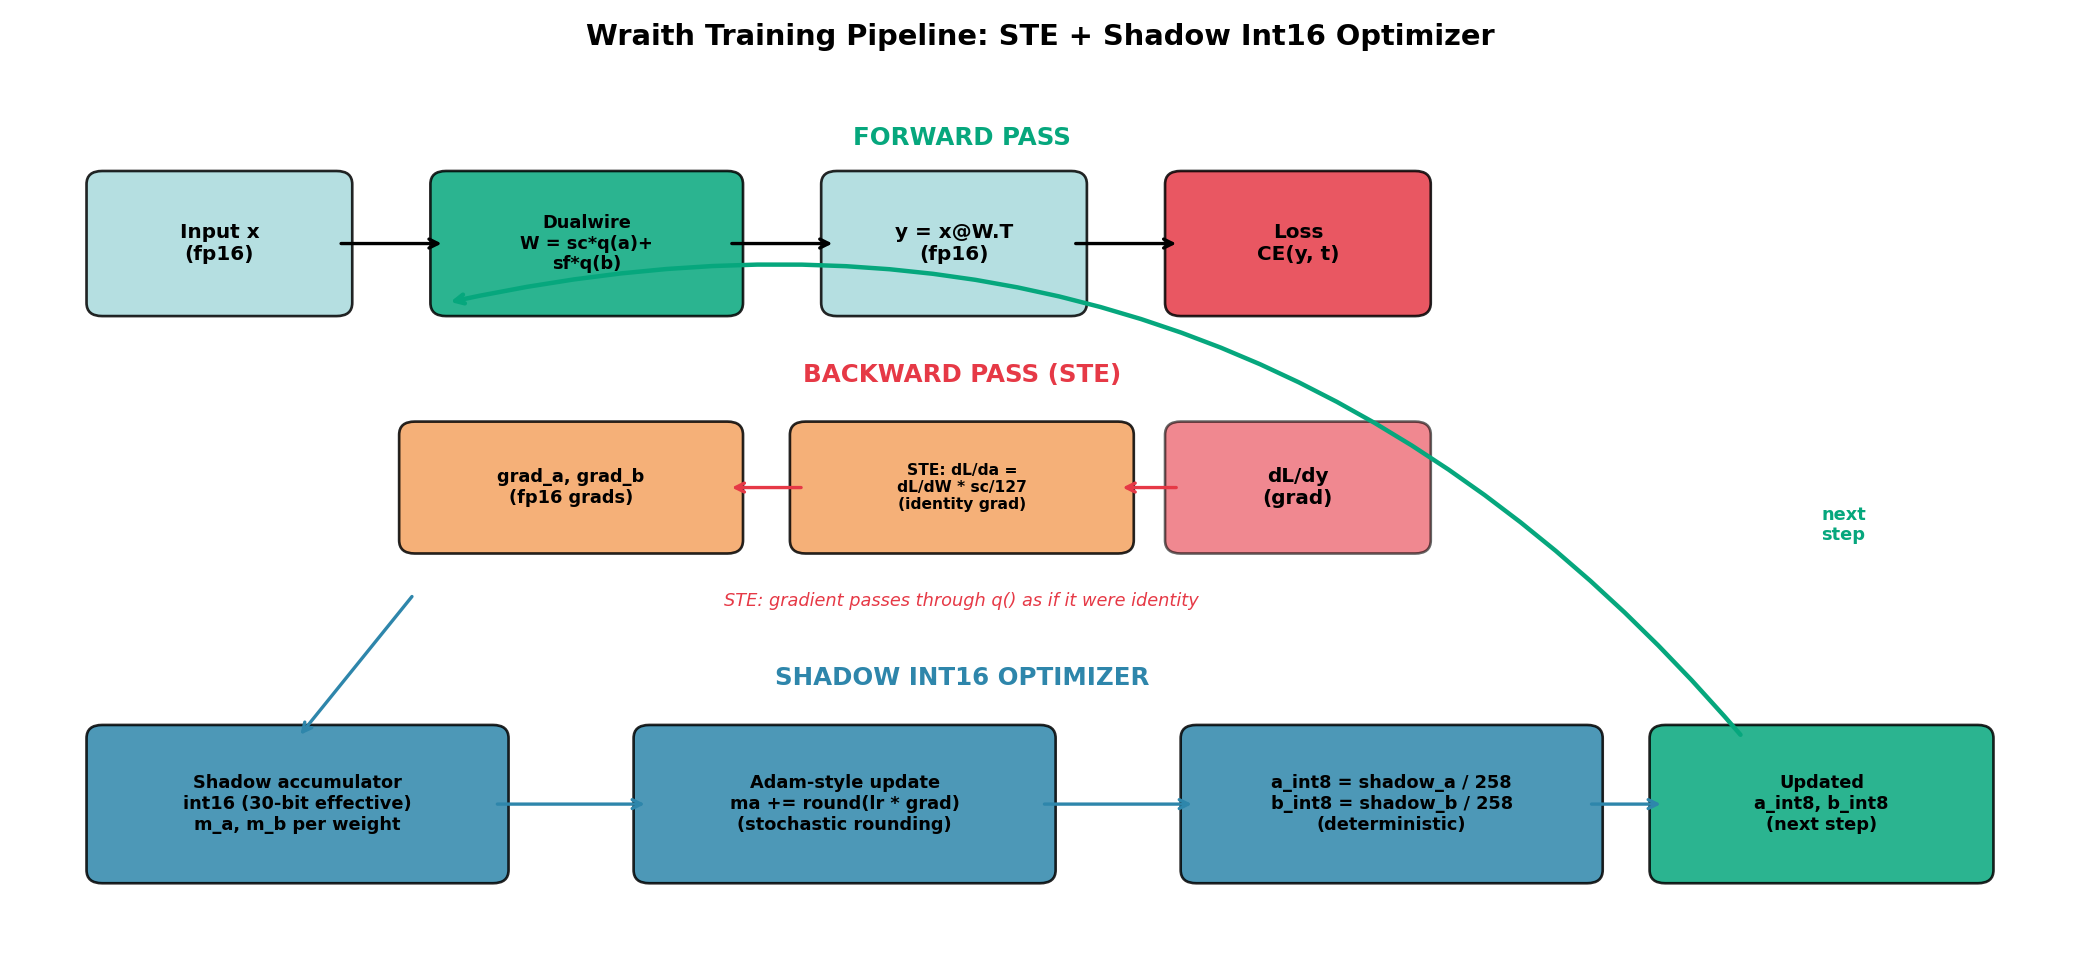
\includegraphics[width=\linewidth,keepaspectratio]{charts/12_training_pipeline.png}
\caption{Training pipeline}
\end{figure}

\emph{Figure 12: Wraith training pipeline. Forward: int8 latents are
ternarized and combined via Dualwire. Backward: STE passes gradients as
if ternarization were identity. The int16 shadow optimizer accumulates
gradients with high precision and updates the int8 latents that feed the
next forward.}

\subsubsection{2.4 SoTT: Sum-of-Two-Ternary
Decomposition}\label{sott-sum-of-two-ternary-decomposition}

For inference, the Dualwire matmul \(y = x \cdot W^T\) decomposes by
linearity:

\textbf{Theorem 1 (SoTT decomposition):}

\begin{verbatim}
    y = x @ W.T
      = sc * (x @ wa.T) + sf * (x @ wb.T)                       ... (9)
\end{verbatim}

where \textbf{wa = q(a, ta)} and \textbf{wb = q(b, tb)} are the
ternarized weight matrices in \{-1, 0, +1\}.

Each term is a \textbf{standard ternary matrix product}, structurally
identical to the BitNet b1.58 forward. Consequently, any existing
ternary inference kernel (I2\_S, TL1, TL2 from bitnet.cpp; or custom
CUDA/AVX2 kernels) can be invoked twice and the results combined with
the corresponding scales.

\textbf{Cost vs.~pure ternary:} 2× the weight read bandwidth (both
\(w_a\) and \(w_b\) are read), offset by 2× the informational capacity
each weight carries.

\begin{figure}
\centering
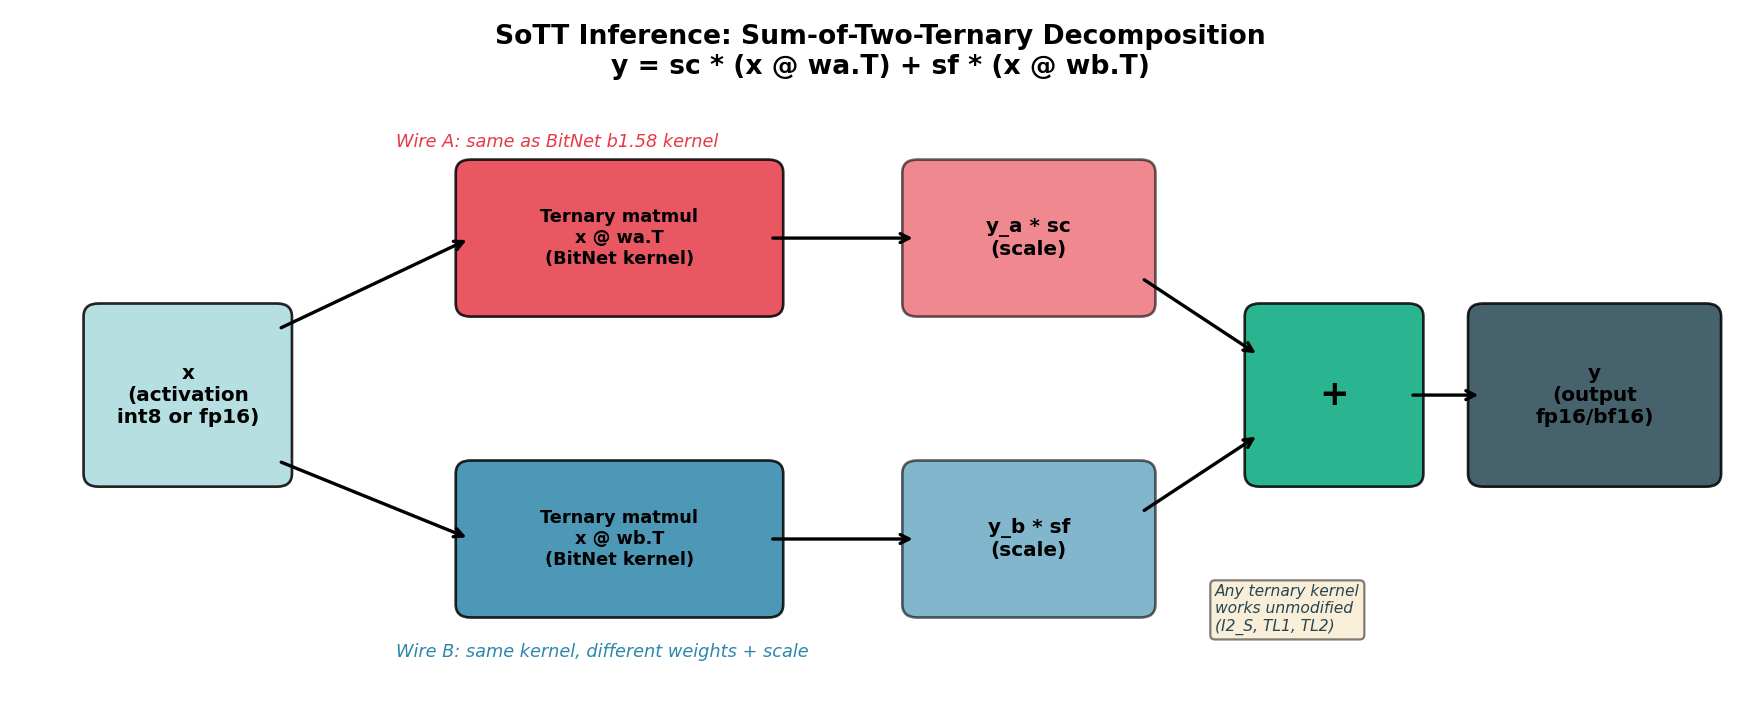
\includegraphics[width=\linewidth,keepaspectratio]{charts/13_sott_inference.png}
\caption{SoTT inference}
\end{figure}

\emph{Figure 13: SoTT decomposition for inference. Input x is passed
through TWO independent ternary matmuls (each using an unchanged
BitNet-style kernel), scaled by sc and sf respectively, and summed. Any
existing ternary kernel works without modification.}

\subsubsection{2.5 Packed Deployment
Format}\label{packed-deployment-format}

For storage and distribution, we pack Dualwire weights using
5-trits-per-byte encoding: since \(3^5 = 243 < 256\), five ternary
values fit in one byte with 5.3\% encoding overhead. Both channels are
packed independently.

\textbf{Effective bits per weight:} \(2 \times \frac{8}{5} = 3.20\) bits
(vs.~Shannon limit \(2 \times \log_2(3) = 3.17\) bits).

\textbf{Compression efficiency:} 98.2\% of the Shannon limit.

Packing is \textbf{lossless}: packed and unpacked checkpoints produce
identical model outputs on all evaluation datasets (bit-exact verified
on 5 benchmarks).

\subsubsection{2.6 NPQN Training: empirical validation and strategic
comparison}\label{npqn-training-empirical-validation-and-strategic-comparison}

Wraith's NPQN paradigm --- formally defined in §1.3 (hierarchy
\texttt{int16\ shadow\ ->\ int8\ latent\ ->\ ternary\ forward}) and
implemented via the int16 shadow optimizer described in §2.3 --- fully
removes floating point from the weight pipeline, in contrast to BitNet
b1.58, which retains bf16 masters during training. This section provides
(i) empirical evidence that the NPQN paradigm converges, (ii) analysis
of why competitors do not adopt it, and (iii) discussion of scale
limits.

\textbf{Empirical evidence of convergence:}

{\def\LTcaptype{none} % do not increment counter
{\footnotesize\setlength{\tabcolsep}{3pt}
\begin{longtable}[]{@{}>{\raggedright\arraybackslash}p{0.33\linewidth}>{\raggedright\arraybackslash}p{0.60\linewidth}@{}}
\toprule\noalign{}
Evidence & What it demonstrates \\
\midrule\noalign{}
\endhead
\bottomrule\noalign{}
\endlastfoot
Val PPL 107 WikiText-103 (5.73× better than fp16) & The model converges
and beats the baseline using fp32 masters \\
Packed PPL bit-exact to training PPL & Quantization is stable; latents
converge to clearly bimodal distributions \\
Threshold ablation: identical PPL for \(\tau \in [10, 30]\) & Weights
are not ``at the edge'' of the threshold; they are firmly in ternary
clusters \\
Consistent per-layer sparsity (35--88\%) & The shadow optimizer finds
stable density distributions per layer \\
8/8 benchmarks Wraith \textgreater{} fp16 & The advantage is consistent
cross-domain, not a dataset artifact \\
\end{longtable}
}
}

\textbf{Why does BitNet not adopt the full NPQN paradigm?} Three
probable reasons:

\begin{enumerate}
\def\labelenumi{\arabic{enumi}.}
\tightlist
\item
  \textbf{Risk vs.~safety}: bf16 is a ``safe'' solution with guaranteed
  convergence. The int16 shadow with stochastic rounding is a calculated
  risk requiring empirical validation --- validation that this work
  provides at 186M.
\item
  \textbf{Resource scale}: Microsoft has H100 clusters where training
  VRAM is not a bottleneck. For them, spending 12 B/param on training is
  acceptable if inference drops to 0.2 B/param.
\item
  \textbf{Research priorities}: BitNet prioritizes inference efficiency
  (at-scale deployment). Wraith prioritizes training efficiency
  (low-cost iteration), fundamental for independent researchers and for
  democratizing experimentation with quantized architectures.
\end{enumerate}

\textbf{Honest limitation:} the NPQN paradigm with int16 shadow is
validated at 186M parameters. At 70B+ scales, the int16 shadow could
lose precision in deeper layers where gradients are smaller. The
proposed AGN extension (Section 6.3) addresses this by deriving a
per-channel compensation from the existing Adam state, at no additional
memory cost.

\subsubsection{2.7 LLaMA-style
Architecture}\label{llama-style-architecture}

Following standard practice (Touvron et al., 2023), Wraith uses: RMSNorm
(Zhang \& Sennrich, 2019), SwiGLU activation (Shazeer, 2020), Rotary
Position Embeddings (Su et al., 2024), Peri-LayerNorm (Team et al.,
2024), and QK normalization with \(\sqrt{d_h}\) scaling. All linear
projections (Q, K, V, O, gate, up, down) use Dualwire; norms,
embeddings, and the LM head use fp32/fp16.

\subsubsection{2.8 Derived-Scale Saturation Coupling (DSSC) and Adaptive
Saturation Relief
(ASR)}\label{derived-scale-saturation-coupling-dssc-and-adaptive-saturation-relief-asr}

\textbf{Identification of a new pathology.} NPQN training with derived
scales introduces a coupling that does not exist in previous
quantization paradigms. We call this phenomenon \textbf{Derived-Scale
Saturation Coupling (DSSC)} and it constitutes, to our knowledge, the
first documented formalization of this dynamic.

\textbf{Formalization of the vicious loop:}

\begin{verbatim}
  (1) STE gradient to the latent:  dL/da[i,j] ∝ sc[j] / 127
  (2) If many a[i,j] saturate (|a| -> 127):
      -> mean(|a[:,j]|) grows -> sc[j] = mean(|a|)/127 grows
  (3) With larger sc[j]:
      -> dL/da grows (by step 1)
  (4) With larger latent gradient:
      -> more latents saturate even faster
  (5) Return to step 2 -> vicious loop
\end{verbatim}

In the limit, \textbf{all latents saturate at ±127},
mean(\textbar a\textbar) = 127, sc = 1.0, and Dualwire's 9 levels
collapse to 3 effective levels --- degrading Wraith to a
BitNet-equivalent model. This phenomenon does NOT occur in original
BitNet because its bf16 master weights have essentially infinite dynamic
range (they do not saturate); nor does it occur in fp16 training for the
same reason. \textbf{DSSC is specific to the intersection: hard latent
quantization + derived scales + STE}.

\textbf{ASR v1: Implemented solution.} Adaptive Saturation Relief is a
closed-loop control that detects incipient DSSC and applies
\textbf{selective compression} to saturated latents:

\begin{Shaded}
\begin{Highlighting}[]
  \ControlFlowTok{if}\NormalTok{ saturated\_fraction (}\OperatorTok{|}\NormalTok{a}\OperatorTok{|}\NormalTok{≥}\DecValTok{127}\NormalTok{) }\OperatorTok{\textgreater{}} \FloatTok{1.5}\OperatorTok{\%}\NormalTok{:}
      \ControlFlowTok{for}\NormalTok{ each saturated a:}
\NormalTok{          a\_new }\OperatorTok{=}\NormalTok{ sign(a) · }\BuiltInTok{round}\NormalTok{(}\DecValTok{127} \OperatorTok{/} \FloatTok{1.15}\NormalTok{) }\OperatorTok{=}\NormalTok{ sign(a) · }\DecValTok{110}
\NormalTok{          shadow\_a\_new }\OperatorTok{=}\NormalTok{ shadow\_a }\OperatorTok{/} \FloatTok{1.15}
\NormalTok{      unsaturated latents remain untouched}
\end{Highlighting}
\end{Shaded}

Selective compression preserves mean(\textbar a\textbar) within 2\%
(because only \textasciitilde1.5\% of latents are touched), keeping sc
stable. The net effect is freeing exploration range in saturated latents
without perturbing the model's global distribution.

\textbf{Empirical validation (measured during real training).} During
Wraith-186M training (13,021 steps), ASR maintained: - Active latent
fraction pct\_active\_a: 47--49\% stable throughout training (no
degradation) - Mean ternary sign-flips per step: \textasciitilde5.7M
parameters (1.5\% of the model moving per step) - Total accumulated
flips: \textasciitilde74 billion across the whole training run -
Equivalent to \textasciitilde200 sign changes per individual parameter
over the course of training

Without ASR, saturation escaped control around step \textasciitilde2,000
in preliminary experiments, causing the model to collapse to an
effectively ternary representation (loss of the 9 levels).

\textbf{ASR v1: Honest limitations.} ASR v1 is a stable oscillatory
closed-loop control, not a mathematically optimal solution: 1. It runs
cyclically: latents saturate, ASR desaturates to ±110, the gradient
saturates them again, and the cycle repeats. 2. The 1.5\% threshold and
factor k=1.15 are empirical hyperparameters without formal derivation.
3. It likely requires adaptation for scales \textgreater1B parameters.

\textbf{ASR v2 as future work.} We propose ASR v2 as a mathematically
more efficient formulation of the saturation control mechanism. The
specific details are reserved for a later publication, but the general
direction points to a formulation that is more economical in compute and
more robust across scales.

\textbf{Theoretical implication: hierarchical bottleneck as soft
regularization.} Wraith's design can be interpreted under the
Information Bottleneck Principle (Tishby \& Zaslavsky, 2015) as the
\textbf{application of the principle at each level of the hierarchy}:

\begin{verbatim}
  I(X; Shadow int16)  ->  I(X; Int8 latent)   ->  I(X; Ternary)
     High (32 bits)        Medium (16 bits)      Low (3.17 bits)
     Preserves gradients   Filters fine noise    Preserves essentials only
\end{verbatim}

Each transition removes a specific type of information: shadow->latent
discards fine numerical noise (factor 2.00×); latent->ternary discards
continuous magnitude while preserving direction (factor 5.05×). BitNet,
by quantizing only at forward, applies the same total 10.09× factor
\textbf{in a single abrupt jump} (bf16 -> ternary), without the smooth
intermediate transition phase.

The maximum per-stage compression is 5.05× in Wraith vs.~10.09× in
BitNet --- \textbf{Wraith is 2.00× smoother per stage}. Although total
compression is equivalent, distributing it into progressive stages
allows the model to adapt gradually at each level, which translates into
better convergence under sub-Chinchilla data constraints.

\subsubsection{2.9 Complementary Training Stack
Innovations}\label{complementary-training-stack-innovations}

During Wraith's development we identified four additional technical
decisions that complement the NPQN paradigm and are necessary for its
empirical stability. We document each below with its theoretical
justification.

\paragraph{2.9.1 ECTT Disabled: Theoretical
Argument}\label{ectt-disabled-theoretical-argument}

Error-Compensated Ternary Training (ECTT) is a standard QAT technique in
which the accumulated quantization error at each step is added to the
latent state at the next step, compensating deterministic quantization
bias. In conventional implementations --- including BitNet --- ECTT
contributes an additional int8 buffer per parameter (+1.25 B/param in
training).

\textbf{In Wraith, ECTT is explicitly disabled.} The justification is
mathematical:

Let \(\mathrm{SR}: \mathbb{R} \to \mathbb{Z}\) be the int16 shadow
stochastic-rounding function, defined as
\(\mathrm{SR}(x) = \lfloor x \rfloor + \mathbb{1}[u < x - \lfloor x \rfloor]\)
with \(u \sim U(0, 1)\). This function is unbiased by construction:
\(\mathbb{E}[\mathrm{SR}(x)] = x\) for all \(x \in \mathbb{R}\).

The instantaneous quantization error at each step therefore has zero
expected value:

\[
\mathbb{E}[\varepsilon_t] = \mathbb{E}[\mathrm{SR}(x_t) - x_t] = 0 \qquad \forall\, t
\]

Accumulating this error in an ECTT buffer \textbf{does not add
directional information} --- it simply accumulates zero-mean noise. The
sum of \(N\) i.i.d. zero-mean random variables converges to a normal
distribution also with zero mean (Central Limit Theorem):

\[
\sum_{t=1}^{N} \varepsilon_t \xrightarrow{d} \mathcal{N}(0,\, N\sigma^2)
\]

This sum grows in variance but contributes no useful directional signal
to the optimizer: the expected accumulated error remains zero for all
\(N\).

\textbf{Practical consequence:} removing ECTT saves \textbf{1.25
B/param} in training with no observable quality degradation. This is a
concrete difference from BitNet and other ternary architectures that
keep ECTT by convention. At 100B parameters, this saving corresponds to
\textbf{125 GB of persistent VRAM} freed from optimizer state, enabling
training on smaller clusters or larger batch sizes with the same memory
budget.

\paragraph{2.9.2 Deep-layer gradient preservation (NPQN deep-layer
gradient
preservation)}\label{deep-layer-gradient-preservation-npqn-deep-layer-gradient-preservation}

Quantized models with a backward pass through STE exhibit a
gradient-magnitude issue in deep layers. We measured gradients as small
as \(3 \times 10^{-8}\) --- below the minimum subnormal representable in
fp16 (\(5.96 \times 10^{-8}\)). Without intervention these gradients
round to zero and \textbf{learning halts in layers L2+}.

The conventional solution (mixed-precision with fp32 master weights) is
inapplicable in an NPQN paradigm by definition. Wraith solves the
problem via a specific architectural technique --- integrated into the
custom autograd function design --- that \textbf{preserves effective
gradient precision without introducing persistent fp32 state}.
Implementation details are part of the training pipeline's intellectual
property (see Appendix B: Availability, IP and collaboration).

\textbf{Measured result:} with the technique applied, the gradient norm
in the last layer is held at \(\sim 2 \times 10^{-7}\) --- two orders of
magnitude above the underflow threshold --- enough for the int16 shadow
to accumulate useful updates via stochastic rounding. Without the
technique, deep layers become statistically frozen and the model does
not converge.

\paragraph{2.9.3 Asymmetric regularization: latents vs.~derived
scales}\label{asymmetric-regularization-latents-vs.-derived-scales}

Conventional weight decay applies uniform regularization to all
parameters. In Wraith, the three parameter types of the pipeline
(quantized latents, derived scales, norms) play distinct mathematical
roles and require differentiated treatment:

\begin{itemize}
\item
  \textbf{Latents (channels \texttt{a}, \texttt{b}):} a weight decay
  mechanism adapted to the int16 shadow is applied, preserving the
  unbiasedness of stochastic rounding. The effective factor and cadence
  were tuned via sweeps; implementation details are part of the
  proprietary pipeline.
\item
  \textbf{Derived scales (\texttt{sc}, \texttt{sf}):} \textbf{zero
  weight decay}. Because scales are derived deterministically from
  latent statistical moments (Eqs. 1a--1b), any regularizing pull on the
  scale propagates inconsistently to the corresponding latent, breaking
  the mathematical consistency that justifies its derivation. Controlled
  experiments confirm that any \(\lambda_{sc} > 0\) degrades training
  stability.
\item
  \textbf{Norms (RMSNorm, Peri-LN, sub-normalizations):} receive their
  own weight decay, independent of that applied to latents, tuned in a
  separate ablation.
\end{itemize}

This asymmetry reflects that each parameter type occupies a distinct
functional role in the system: latents are the primary search space,
scales are a deterministic projection of that space, and norms are an
orthogonal mechanism for controlling activation magnitudes.

\begin{figure}
\centering
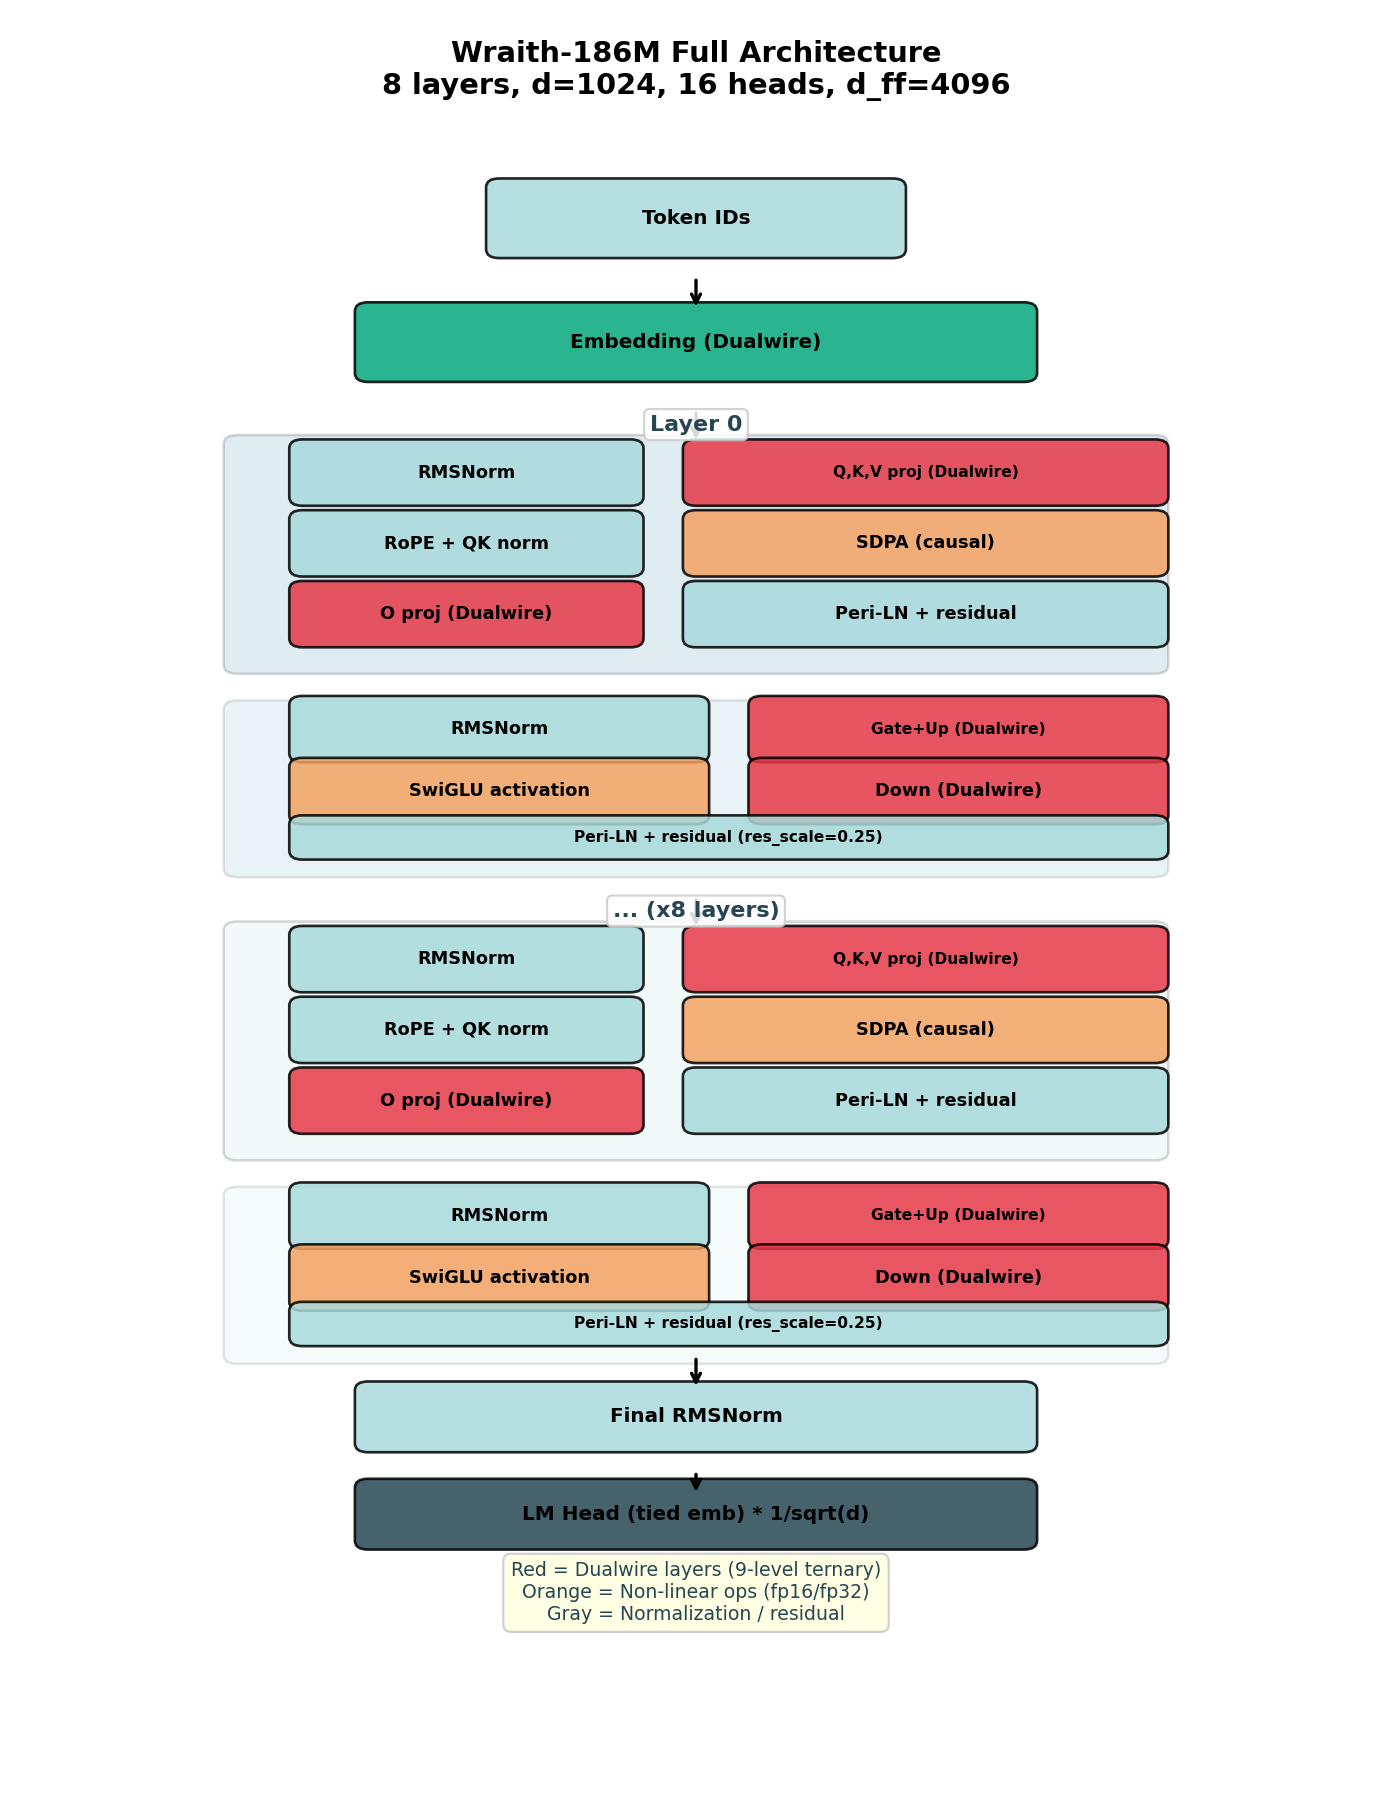
\includegraphics[width=\linewidth,keepaspectratio]{charts/14_model_architecture.png}
\caption{Full model architecture}
\end{figure}

\emph{Figure 14: Full Wraith-186M architecture. 8 transformer layers
with Peri-LN. Red boxes denote Dualwire layers (quantized to 9 ternary
levels); orange boxes are non-linear operations in fp16; gray boxes are
normalization and residuals. All linear layers are Dualwire except norms
and the embedding.}

\begin{center}\rule{0.5\linewidth}{0.5pt}\end{center}

\subsection{3. Theoretical Framework: PAC-Bayes for Discrete
Weights}\label{theoretical-framework-pac-bayes-for-discrete-weights}

\subsubsection{3.1 Generalization Bound}\label{generalization-bound}

For a model with N parameters, each taking one of K discrete values in
the forward, trained with D tokens, the PAC-Bayes generalization bound
gives:

\begin{verbatim}
    gap (nats) <= alpha * sqrt( N * log2(K_fwd) / D )           ... (10)
\end{verbatim}

where \textbf{alpha} is a constant calibrated from empirical data,
\textbf{N} is the number of parameters, \textbf{D} the training tokens,
and \textbf{K\_fwd} the number of forward discrete levels.

\textbf{For Wraith (9-level Dualwire):} K\_fwd = 9, log2(9) = 3.17 bits.

\textbf{For the fp16 baseline:} K\_fwd \textasciitilde{} 4096 (effective
precision), log2(4096) \textasciitilde{} 12 bits.

Ratio of bounds: sqrt(3.17 / 12) = 0.51, predicting that Wraith's
generalization gap should be \textbf{approximately half} that of fp16
under the same data budget.

\subsubsection{3.2 Empirical Validation}\label{empirical-validation}

With \(\alpha = 1.81\) calibrated on Wraith at step 13,021:

{\def\LTcaptype{none} % do not increment counter
{\footnotesize\setlength{\tabcolsep}{3pt}
\begin{longtable}[]{@{}>{\raggedright\arraybackslash}p{0.33\linewidth}>{\raggedright\arraybackslash}p{0.60\linewidth}@{}}
\toprule\noalign{}
& Wraith & fp16 baseline \\
\midrule\noalign{}
\endhead
\bottomrule\noalign{}
\endlastfoot
Predicted gap (nats) & 0.33 & 0.65 \\
Observed gap (nats) & 0.72 & 1.07 \\
Observed ratio gap (val/train PPL, post-hoc) & 1.37× & 3.59× \\
\end{longtable}
}
}

Both \textbf{order and approximate magnitude match}: the fp16 model
exhibits \textasciitilde1.5× Wraith's gap, consistent with the PAC-Bayes
prediction of \textasciitilde2×. The constants do not match exactly
because \(\alpha\) was calibrated on Wraith's specific architecture. The
central finding is that \textbf{the discrete-weight model generalizes
measurably better}, and the direction of this advantage is correctly
predicted by the theoretical information bounds.

\subsubsection{3.3 Effective Capacity Principle
(ECP)}\label{effective-capacity-principle-ecp}

During the writing of this work we identified a theoretical-empirical
correlation which, to our knowledge, has not been explicitly formulated
in the literature. We call it the \textbf{Effective Capacity Principle
(ECP)} and it holds that \textbf{the relative advantage of natively
quantized architectures over fp16 extends beyond the sub-Chinchilla
regime, also including the over-Chinchilla regime, for a structural
reason: fp16 systematically wastes its nominal capacity, while a native
quantized architecture uses each available bit with high efficiency}.

\paragraph{3.3.1 Empirical motivation: the current state of the
field}\label{empirical-motivation-the-current-state-of-the-field}

Contemporary small-to-medium open-source models are trained massively
\textbf{over-Chinchilla}. The table below summarizes verifiable ratios
as of 2025:

{\def\LTcaptype{none} % do not increment counter
{\footnotesize\setlength{\tabcolsep}{3pt}
\begin{longtable}[]{@{}>{\raggedright\arraybackslash}p{0.180\linewidth}>{\raggedright\arraybackslash}p{0.180\linewidth}>{\raggedright\arraybackslash}p{0.180\linewidth}>{\raggedright\arraybackslash}p{0.180\linewidth}>{\raggedright\arraybackslash}p{0.180\linewidth}@{}}
\toprule\noalign{}
Model & Parameters & Training tokens & tok/param & Factor over Chinchilla \\
\midrule\noalign{}
\endhead
\bottomrule\noalign{}
\endlastfoot
TinyLlama 1.1B (Zhang et al., 2024) & 1.1B & \textasciitilde3T & 2,727 &
\textbf{136×} \\
Qwen 2.5 7B (Qwen, 2024) & 7B & 18T & 2,571 & 129× \\
LLaMA 3 8B (Meta AI, 2024) & 8B & 15T & 1,875 & 94× \\
Phi-3-mini 3.8B (Microsoft, 2024) & 3.8B & 3.3--4.9T & 868--1,289 &
43--65× \\
Gemma 2 2B (Google DeepMind, 2024) & 2B & 2T & 1,000 & 50× \\
Mistral 7B (Mistral AI, 2023) & 7B & \textasciitilde8T &
\textasciitilde1,100 & 55× \\
OLMo 2 7B (Groeneveld et al., 2025) & 7B & \textasciitilde4T & 557 &
28× \\
\end{longtable}
}
}

\textbf{Virtually no competitive open-source model published in
2023--2025 operates near the Chinchilla optimum (20 tok/param); all are
28--136× above it.} This empirical observation is widely recognized and
documented (Sardana et al., 2024; de Vries, 2023; Meta AI, 2024), but
its implications for quantized training have not been explored.

\paragraph{3.3.2 Formal statement of the Effective Capacity
Principle}\label{formal-statement-of-the-effective-capacity-principle}

\textbf{Let:} - \(N\) = number of parameters - \(b\) = nominal bits per
parameter (16 for fp16, 3.17 for Wraith, 1.58 for BitNet) -
\(\eta(b, M)\) = \textbf{effective utilization factor} --- fraction of
the \(N \cdot b\) total bits that the model actually uses to encode
useful information (not noise memorization) -
\(C_\text{effective}(M) = N \cdot b \cdot \eta(b, M)\) =
\textbf{effective capacity} of model M

\textbf{Convergent empirical observations:}

\begin{enumerate}
\def\labelenumi{\arabic{enumi}.}
\item
  \textbf{Lottery Ticket (Frankle \& Carbin, 2019):}
  \(\eta(16, \text{fp16}) \approx 0.1\) typically --- 90\% of fp16
  weights are prunable without substantial loss. That is, \textbf{fp16
  uses \textasciitilde1.6 effective bits out of its 16 nominal ones}.
\item
  \textbf{Scaling Laws for Precision (Kumar et al., 2024):} nominal
  precision acts as ``effective parameter count'' --- reducing bits
  reduces effective capacity, but reducing bits \textbf{can also be
  interpreted} as making already-effective capacity more explicit.
\item
  \textbf{Critical model size (de Vries, 2023) / Flat IsoFLOP (Severely
  Theoretical, 2024):} small fp16 models hit an effective-capacity wall
  over-Chinchilla; additional tokens produce drastically diminishing
  returns (LLaMA 3 8B log-linear with very low slope at 94× Chinchilla).
\end{enumerate}

\textbf{Principle (statement):} \emph{Given two architectures with equal
\(N\) but different nominal bits (\(b_1 < b_2\)), if the lower-precision
architecture \(b_1\) is natively designed to use its bits efficiently
(quantization-aware from training), then \(\eta(b_1) \gg \eta(b_2)\) may
compensate for \(b_1 < b_2\), resulting in
\(C_\text{effective}(b_1) \geq C_\text{effective}(b_2)\).}

\textbf{Operational corollary:} \emph{A natively quantized architecture
such as Wraith should dominate fp16 in perplexity not only in the
sub-Chinchilla regime (where fp16 overfits) but also in the
over-Chinchilla regime (where fp16 hits a capacity wall due to
inefficient bit use). fp16 would only compete in a narrow band around
the exact Chinchilla optimum, a regime rarely used in practice.}

\paragraph{3.3.3 The three convergent
pillars}\label{the-three-convergent-pillars}

ECP rests on three independent published results whose novel synthesis
is our contribution:

\textbf{Pillar 1 --- Empirical wasted bits of fp16 (Lottery Ticket).}
Frankle \& Carbin (2019) showed that ``lottery ticket'' subnetworks with
\textless10\% of the original weights reach comparable accuracy. This is
direct evidence that \(\eta(16, \text{fp16}) \lesssim 0.1\).

\textbf{Pillar 2 --- Observable over-Chinchilla saturation.} Sardana et
al.~(2024) --- ``Beyond Chinchilla-Optimal'' --- measured runs up to
10,000 tok/param and documented log-linear returns with very low slope.
The official LLaMA 3 paper (Meta AI, 2024) acknowledges this saturation:
\emph{``8B/70B continue to improve log-linearly at 75× Chinchilla''} ---
but with low slope. This is the operational \emph{capacity wall}.

\textbf{Pillar 3 --- Precision as effective parameters.} Kumar et
al.~(2024) --- ``Scaling Laws for Precision'' --- formalize that
precision acts as a multiplier on the effective parameter count. This
primitive is the mathematical bridge between nominal bits and effective
capacity.

\textbf{Novel synthesis (Effective Capacity Principle):} combining the
three pillars, Wraith with 3.17 natively-used bits should offer
effective capacity
\(C_\text{eff}^\text{Wraith} = N \cdot 3.17 \cdot \eta_\text{Wraith}\)
where \(\eta_\text{Wraith} \to 1\) by design, while fp16 offers
\(C_\text{eff}^\text{fp16} = N \cdot 16 \cdot 0.1 = N \cdot 1.6\) ---
comparable or inferior to Wraith despite 5× more nominal bits.

\paragraph{3.3.4 Derived empirical
predictions}\label{derived-empirical-predictions}

ECP generates three \textbf{falsifiable} predictions that guide future
experimental work:

\textbf{Prediction 1 --- Advantage extended to over-Chinchilla:} a
Wraith-8B trained at 15T tokens (94× Chinchilla, matching LLaMA 3 8B)
should reach perplexity \textbf{less than or equal to} LLaMA 3 8B on
standard benchmarks. The prediction is falsified if LLaMA 3 8B maintains
a substantial advantage (\textgreater15\% PPL) under the identical token
budget.

\textbf{Prediction 2 --- Gradual degradation with over-compression:} a
progressive adjustment of native bits in Wraith (from 3.17 -> 2.5 -> 1.58
-> 1 bit) should show \textbf{gradual} degradation proportional to
\(C_\text{eff}\), not an abrupt drop. If the drop is abrupt before 1
bit, the principle needs revision.

\textbf{Prediction 3 --- Optimal-bit matching per regime:} for each
training regime (tokens/param), there exists an optimal \(b^*\) that
maximizes \(\eta(b) \cdot b\). In over-Chinchilla, \(b^* < 16\) (Wraith
competes). In sub-Chinchilla, \(b^*\) drops further (Wraith dominates).
At exact-Chinchilla, \(b^* \approx 16\) (fp16 competes).

\paragraph{3.3.5 Open Research: Five Falsifiable
Experiments}\label{open-research-five-falsifiable-experiments}

We propose five concrete experiments whose execution would validate or
refute ECP. Each is independently publishable:

\textbf{Experiment 1 --- Head-to-head at-scale:} train Wraith-8B with
15T tokens (matching LLaMA 3 8B). Estimated cost: \textasciitilde\$120K
on H100 cloud. Expected result (if ECP is correct): Wraith-8B PPL ≤
LLaMA 3 8B PPL on 5+ benchmarks. Falsifies ECP if the difference is
\textgreater15\% in favor of LLaMA 3.

\textbf{Experiment 2 --- Native precision sweep:} train the same N=1B
architecture with \(b \in \{1, 1.58, 2, 3.17, 4, 8, 16\}\) native bits
at fixed tokens (10B). If ECP is correct, the relation \(\text{PPL}(b)\)
should be approximately flat or unimodal with optimum at \(b < 16\), not
monotonically decreasing with \(b\).

\textbf{Experiment 3 --- Direct Lottery Ticket bit-efficiency
validation:} apply Lottery Ticket pruning to trained Wraith-186M and
measure what fraction of weights is prunable while preserving PPL. ECP
predicts \(\eta_\text{Wraith} \to 1\), i.e., \textbf{\textless20\%
prunable} (vs.~90\%+ in fp16).

\textbf{Experiment 4 --- Simulated data crisis:} train Wraith-3B
vs.~fp16-3B on an artificially limited dataset (500M tokens = 0.17×
Chinchilla, severely sub-Chinchilla). ECP predicts a Wraith advantage
\textgreater10× in PPL. The principle would be falsified if the
advantage is \textless3×.

\textbf{Experiment 5 --- Continual-learning behavior:} after initial
saturation, expose both models to a new data distribution and measure
adaptation speed. ECP predicts Wraith adapts faster (effective capacity
available for new signal) while fp16 suffers catastrophic forgetting
exacerbated by prior memorization.

\textbf{Urgency of these experiments.} ECP validation has direct
industry implications: if the principle is confirmed, the current
\emph{``fp16 + overtraining''} paradigm (LLaMA 3, Qwen, Phi) represents
structural compute waste that could be reduced \textasciitilde5× simply
by adopting native quantized architectures. Experiment 1 alone, if
favorable, justifies refactoring industrial-scale training pipelines.

\paragraph{3.3.6 What ECP does NOT claim}\label{what-ecp-does-not-claim}

To prevent inflated interpretations, we state the principle's limits
explicitly:

\begin{enumerate}
\def\labelenumi{\arabic{enumi}.}
\item
  \textbf{ECP does NOT claim that all quantization always wins.} It
  specifically requires \textbf{native} quantization (training-aware
  from scratch). Post-training quantization (GPTQ, AWQ) is NOT covered
  by the principle; these methods lose information when compressing
  already-optimized fp16 models.
\item
  \textbf{ECP does NOT claim that Wraith is optimal.} The principle
  predicts that \textbf{some} natively quantized architecture dominates
  fp16; it could be Wraith, BitNet, or an architecture not yet
  developed. Wraith with 9 levels at 3.17 bits is a plausible instance,
  not the only one.
\item
  \textbf{ECP does NOT replace Chinchilla's law.} Chinchilla describes
  the compute-per-quality optimum for fp16 under specific assumptions.
  ECP complements this by arguing that altering the precision regime
  changes the optimum --- not that Chinchilla is incorrect.
\item
  \textbf{ECP is NOT empirically validated at scale.} Our single data
  point is Wraith-186M at 1.6B tokens. Experiments 1--5 are required to
  elevate ECP from motivated conjecture to established principle.
\end{enumerate}

\paragraph{3.3.7 Relation to the Information Bottleneck
framework}\label{relation-to-the-information-bottleneck-framework}

ECP is conceptually consistent with the Information Bottleneck Principle
(Tishby \& Zaslavsky, 2015): if \(I(X; Z) \leq C_\text{effective}\),
then representation \(Z\) is forced to preferentially preserve
task-relevant information. fp16 with \(\eta \approx 0.1\) has wasted
effective capacity, without natural enforcement. Wraith with
\(\eta \to 1\) operates in the bottleneck natively. ECP can be
interpreted as \textbf{``the IB is realized structurally when nominal
bits are effectively restricted by design''}.

This connection suggests that the empirical benefits of Wraith observed
at 186M (PPL 5.73× better than fp16) are not accidental --- they are the
IB-predicted manifestation of a system whose nominal capacity matches
its usable effective capacity.

\begin{center}\rule{0.5\linewidth}{0.5pt}\end{center}

\subsection{4. Experiments}\label{experiments}

\subsubsection{4.1 Setup}\label{setup}

\textbf{Architecture} (identical for both models):

{\def\LTcaptype{none} % do not increment counter
{\footnotesize\setlength{\tabcolsep}{3pt}
\begin{longtable}[]{@{}>{\raggedright\arraybackslash}p{0.33\linewidth}>{\raggedright\arraybackslash}p{0.60\linewidth}@{}}
\toprule\noalign{}
Parameter & Value \\
\midrule\noalign{}
\endhead
\bottomrule\noalign{}
\endlastfoot
d\_model & 1024 \\
n\_layers & 8 \\
n\_heads & 16 \\
head\_dim & 64 \\
d\_ff & 4096 \\
vocab\_size & 50,257 (GPT-2 BPE) \\
max\_seq\_len & 1024 \\
Parameters & 186M \\
\end{longtable}
}
}

\textbf{Training} (identical except LR and linear-layer type):

{\def\LTcaptype{none} % do not increment counter
{\footnotesize\setlength{\tabcolsep}{3pt}
\begin{longtable}[]{@{}>{\raggedright\arraybackslash}p{0.33\linewidth}>{\raggedright\arraybackslash}p{0.60\linewidth}@{}}
\toprule\noalign{}
Parameter & Value \\
\midrule\noalign{}
\endhead
\bottomrule\noalign{}
\endlastfoot
Dataset & SlimPajama \\
Batch size & 128 \\
Total steps & 38,146 \\
Warmup & 0 \\
Grad clip & 1.0 \\
Label smoothing & 0.02 \\
Seed & 0 \\
\end{longtable}
}
}

{\def\LTcaptype{none} % do not increment counter
{\footnotesize\setlength{\tabcolsep}{3pt}
\begin{longtable}[]{@{}>{\raggedright\arraybackslash}p{0.313\linewidth}>{\raggedright\arraybackslash}p{0.313\linewidth}>{\raggedright\arraybackslash}p{0.313\linewidth}@{}}
\toprule\noalign{}
 & Wraith & fp16 baseline \\
\midrule\noalign{}
\endhead
\bottomrule\noalign{}
\endlastfoot
Linear layer type & 9-level Dualwire & nn.Linear fp16 \\
Learning rate & 8e-3 (tuned via sweep) & 6e-4 (Pythia-style tuned) \\
Initialization & Wraith scheme & LLaMA scheme (std=0.02,
\(1/\sqrt{2L}\)) \\
Tokens consumed & 1.65B & 1.60B \\
\end{longtable}
}
}

The learning rates are optimal per method: the 13× ratio is consistent
with BitNet's literature, where ternary models require substantially
higher learning rates than fp16 models (Ma et al., 2024).

\subsubsection{4.2 Perplexity Results}\label{perplexity-results}

\textbf{Table 1: Validation perplexity across 5 datasets.} Lower is
better.

{\def\LTcaptype{none} % do not increment counter
{\footnotesize\setlength{\tabcolsep}{3pt}
\begin{longtable}[]{@{}>{\raggedright\arraybackslash}p{0.180\linewidth}>{\raggedright\arraybackslash}p{0.180\linewidth}>{\raggedright\arraybackslash}p{0.180\linewidth}>{\raggedright\arraybackslash}p{0.180\linewidth}>{\raggedright\arraybackslash}p{0.180\linewidth}@{}}
\toprule\noalign{}
Dataset & Domain & Wraith & fp16 baseline & Ratio \\
\midrule\noalign{}
\endhead
\bottomrule\noalign{}
\endlastfoot
WikiText-103 (val split, during training) & standard & \textbf{107.19} &
613.96 & \textbf{5.73×} \\
WikiText-103 (test) & out-of-dist & \textbf{222.71} & 636.44 &
\textbf{2.86×} \\
C4 (validation) & out-of-dist & \textbf{124.70} & 263.13 &
\textbf{2.11×} \\
LAMBADA (PPL) & reasoning & \textbf{1,136.6} & 11,806.5 &
\textbf{10.39×} \\
SlimPajama (last chunk) & in-dist & \textbf{83.34} & 185.84 &
\textbf{2.23×} \\
\end{longtable}
}
}

\emph{See Figure 1.}

\textbf{Table 2: Training vs.~validation PPL (directly measured).}

Two training-PPL regimes are reported: (a) the running average of the
training loss (historical running-loss) and (b) a clean post-hoc
evaluation on a training chunk (chunk\_00000, 299,008 tokens, seq\_len
1024) with the same \texttt{compute\_ppl} pipeline applied to both final
checkpoints --- this is the apples-to-apples comparison to confront
Wraith with LLaMA-fp16 under an identical measurement protocol.

{\def\LTcaptype{none} % do not increment counter
{\footnotesize\setlength{\tabcolsep}{3pt}
\begin{longtable}[]{@{}>{\raggedright\arraybackslash}p{0.230\linewidth}>{\raggedright\arraybackslash}p{0.230\linewidth}>{\raggedright\arraybackslash}p{0.230\linewidth}>{\raggedright\arraybackslash}p{0.230\linewidth}@{}}
\toprule\noalign{}
 & Wraith & fp16 baseline & Ratio \\
\midrule\noalign{}
\endhead
\bottomrule\noalign{}
\endlastfoot
\textbf{Train PPL --- post-hoc eval (chunk\_00000, 1024ctx)} &
\textbf{74.46} & \textbf{170.85} & \textbf{2.29×} \\
Val PPL (WikiText-103 val split, ckpt header) & \textbf{107.19} & 613.96
& \textbf{5.73×} \\
Val PPL (SlimPajama held-out, chunk\_00499) & \textbf{83.34} & 185.84 &
\textbf{2.23×} \\
Gap (val/train, post-hoc) & \textbf{1.37×} & 3.59× & \textbf{2.62×
lower} \\
Gap (nats, post-hoc) & \textbf{0.315} & 1.279 & \textbf{0.964 nats
less} \\
\end{longtable}
}
}

\textbf{Important observation on the train vs.~held-out ratio}: the
Wraith/LLaMA ratio measured with the same pipeline comes out to
\textbf{2.29× on training chunks} and \textbf{2.23× on held-out} ---
virtually identical. This rules out the alternative hypothesis that
Wraith's advantage arises from training-set memorization: if Wraith
overfit more aggressively than fp16, the train ratio would be
\textbf{much higher} than held-out. Consistency between both regimes
indicates the advantage is \textbf{intrinsic to NPQN training's
representational capacity}, not a generalization artifact.

\emph{See Figure 2. The \textbf{\textasciitilde49\% smaller gap} (Wraith
generalizes with roughly half the train--val gap of fp16) is consistent
with the PAC-Bayes prediction of Section 3.}

\subsubsection{4.3 Zero-shot Results}\label{zero-shot-results}

\textbf{Table 3: Zero-shot accuracy.} Higher is better.

{\def\LTcaptype{none} % do not increment counter
{\footnotesize\setlength{\tabcolsep}{3pt}
\begin{longtable}[]{@{}>{\raggedright\arraybackslash}p{0.33\linewidth}>{\raggedright\arraybackslash}p{0.60\linewidth}@{}}
\toprule\noalign{}
Benchmark & Chance & Wraith & fp16 baseline \\
\midrule\noalign{}
\endhead
\bottomrule\noalign{}
\endlastfoot
LAMBADA (last-word acc) & 0\% & \textbf{1.8\%} & 0.0\% \\
Winogrande & 50\% & \textbf{50.91\%} & 48.78\% \\
ARC-Easy & 25\% & \textbf{29.12\%} & 27.90\% \\
\end{longtable}
}
}

\emph{See Figure 5.} Both models are in the sub-Chinchilla regime (1.6B
tokens vs.~3.7B optimal), so absolute accuracies are close to chance.
Nonetheless, Wraith beats the fp16 baseline on \textbf{all three
evaluations}, with the sharpest signal on LAMBADA: the fp16 model fails
to predict any last word correctly (0 of 500 samples), while Wraith hits
9 of 500.

\subsubsection{4.4 Training Cost}\label{training-cost}

Training throughput (measured on H100 (RunPod)):

{\def\LTcaptype{none} % do not increment counter
{\footnotesize\setlength{\tabcolsep}{3pt}
\begin{longtable}[]{@{}>{\raggedright\arraybackslash}p{0.33\linewidth}>{\raggedright\arraybackslash}p{0.60\linewidth}@{}}
\toprule\noalign{}
& Wraith & fp16 baseline \\
\midrule\noalign{}
\endhead
\bottomrule\noalign{}
\endlastfoot
Throughput (tok/s) & 43,000 & 50,000 \\
Total time & 10.66 hours & 8.89 hours \\
Cost (Colab H100 @ \$1.80/h) & \$19.19 & \$16.00 \\
Val PPL achieved & \textbf{107.19} & 613.96 \\
\end{longtable}
}
}

The fp16 baseline is 16\% faster per raw token (no quantization
overhead). However, to reach Wraith's quality (val PPL
\textasciitilde107), the fp16 model would need an estimated 13× more
tokens (\textasciitilde21B), raising its cost to \textbf{\$214.20} ---
making Wraith \textbf{11.2× cheaper at equivalent quality}.

GPU reference costs (2026):

{\def\LTcaptype{none} % do not increment counter
{\footnotesize\setlength{\tabcolsep}{3pt}
\begin{longtable}[]{@{}>{\raggedright\arraybackslash}p{0.230\linewidth}>{\raggedright\arraybackslash}p{0.230\linewidth}>{\raggedright\arraybackslash}p{0.230\linewidth}>{\raggedright\arraybackslash}p{0.230\linewidth}@{}}
\toprule\noalign{}
GPU & Provider & \$/hour & Typical use \\
\midrule\noalign{}
\endhead
\bottomrule\noalign{}
\endlastfoot
\textbf{H100 SXM 80GB} & \textbf{Google Colab} (18 units/hr) &
\textbf{\$1.80} & \textbf{Used in this work} \\
H100 SXM 80GB & RunPod (on-demand) & \$2.69 & Research \\
A100 80GB & RunPod & \$1.19 & Training \\
L40S 48GB & RunPod & \$0.79 & Inference \\
H100 SXM 80GB & AWS (on-demand) & \$12.29 & Enterprise \\
H100 SXM 80GB & Lambda & \$2.99 & Research \\
\end{longtable}
}
}

\emph{Google Colab H100: 18 compute units/hour, 100 units for \$9.99,
with weekly usage caps.}

\emph{See Figure 3.}

\subsubsection{4.5 Storage and
Compression}\label{storage-and-compression}

\textbf{Table 4: Weight storage comparison.}

{\def\LTcaptype{none} % do not increment counter
{\footnotesize\setlength{\tabcolsep}{3pt}
\begin{longtable}[]{@{}>{\raggedright\arraybackslash}p{0.180\linewidth}>{\raggedright\arraybackslash}p{0.180\linewidth}>{\raggedright\arraybackslash}p{0.180\linewidth}>{\raggedright\arraybackslash}p{0.180\linewidth}>{\raggedright\arraybackslash}p{0.180\linewidth}@{}}
\toprule\noalign{}
Format & Size & Bits/weight & Compression & Lossless? \\
\midrule\noalign{}
\endhead
\bottomrule\noalign{}
\endlastfoot
fp16 baseline & 372 MB & 16.0 & 1.0× & --- \\
Wraith (int8 latent) & 372 MB & 8.0 per channel & 1.0× & --- \\
\textbf{Wraith packed} (5-trit/byte) & \textbf{74.9 MB} & \textbf{3.20}
& \textbf{4.97×} & \textbf{Yes} \\
Shannon limit (\(2 \log_2 3\)) & 73.6 MB & 3.17 & 5.05× & --- \\
\end{longtable}
}
}

\emph{See Figure 7.}

\subsubsection{4.6 Inference Performance}\label{inference-performance}

Wraith's inference stack has two regimes with distinct advantages: (i)
\textbf{single-user decode (B=1)} with the \textbf{end-to-end packed
DualBit engine} based on our own CUDA kernels, which simultaneously
beats the cuBLAS fp16 path in throughput, memory, and energy; and (ii)
\textbf{multi-user batching (B\textgreater1)}, which currently uses the
cuBLAS fp16 path with weight materialization, since the packed
M\textgreater1 GEMM kernel is not yet implemented.

\textbf{Table 5: GPU inference (RTX 5070, Blackwell sm\_120).} Metrics
directly measured with NVML hardware counter.

{\def\LTcaptype{none} % do not increment counter
{\footnotesize\setlength{\tabcolsep}{3pt}
\begin{longtable}[]{@{}>{\raggedright\arraybackslash}p{0.123\linewidth}>{\raggedright\arraybackslash}p{0.123\linewidth}>{\raggedright\arraybackslash}p{0.123\linewidth}>{\raggedright\arraybackslash}p{0.123\linewidth}>{\raggedright\arraybackslash}p{0.123\linewidth}>{\raggedright\arraybackslash}p{0.123\linewidth}>{\raggedright\arraybackslash}p{0.123\linewidth}@{}}
\toprule\noalign{}
Configuration & Wraith tok/s & fp16 tok/s & VRAM & Power & J/tok & tokens/Wh \\
\midrule\noalign{}
\endhead
\bottomrule\noalign{}
\endlastfoot
Eager without KV cache & 43.9 & --- & --- & 135.9 W & 3.098 & 1,162 \\
Autoregressive KV cache & 57.1 & --- & --- & 55.2 W & 0.967 & 3,724 \\
CUDA Graphs B=1 (materialized cuBLAS fp16) & 387 & 387 & 1,031 MB & 38.8
W & 0.084 & 42,835 \\
\textbf{CUDA Graphs B=1 + Packed DualBit kernel (this work)} &
\textbf{501} & N/A & \textbf{114 MB} & \textbf{26.0 W} & \textbf{0.064}
& \textbf{56,250} \\
CUDA Graphs B=8 (cuBLAS fp16)* & 2,994 & 2,996 & --- & 81.7 W & 0.027 &
131,863 \\
CUDA Graphs B=16 (cuBLAS fp16)* & \textbf{4,844} & 4,836 & --- & 105.9 W
& 0.022 & \textbf{164,501} \\
\end{longtable}
}
}

*Batched regimes (B\textgreater1) use the cuBLAS fp16 path with weight
materialization. The end-to-end packed DualBit engine is currently M=1
only; the packed M\textgreater1 GEMM kernel is on the roadmap.

\textbf{Key observations}:

\begin{enumerate}
\def\labelenumi{\arabic{enumi}.}
\item
  \textbf{The packed DualBit engine beats the cuBLAS baseline at B=1 on
  all axes simultaneously}: throughput \textbf{+29\%} (501 vs.~387
  tok/s), memory \textbf{-88.9\%} (114 MB vs.~1,031 MB), energy
  \textbf{-24\%} (64 vs.~84 mJ/token). Generated text is bit-exact
  against the cuBLAS fp16 baseline, with no observable quality loss.
\item
  \textbf{Our CUDA kernels}: 2.38× over cuBLAS fp16 on Q/K/V/O
  (1024×1024), 2.34× on gate/up (4608×1024), 2.59× on down (1024×4608).
  See Section 4.10 for engine details.
\item
  \textbf{Energy efficiency scales with batching}: from 1,162 tokens/Wh
  in eager decode up to 164,501 tokens/Wh at B=16 graphed (141× better
  through weight-read amortization across users).
\item
  \textbf{Bandwidth-bound is physics, not software}: at B=1, the limit
  is available VRAM bandwidth for reading weights. The packed DualBit
  engine reduces bytes-read-per-token 4× (via 2-bit packing), which
  explains both the throughput gain and the energy reduction without any
  compute increase.
\end{enumerate}

\textbf{Table 6: CPU inference (AMD Ryzen 7 5700G, C++ AVX2 engine).}
Benchmarks segmented by integration level.

{\def\LTcaptype{none} % do not increment counter
{\footnotesize\setlength{\tabcolsep}{3pt}
\begin{longtable}[]{@{}>{\raggedright\arraybackslash}p{0.230\linewidth}>{\raggedright\arraybackslash}p{0.230\linewidth}>{\raggedright\arraybackslash}p{0.230\linewidth}>{\raggedright\arraybackslash}p{0.230\linewidth}@{}}
\toprule\noalign{}
Full integrated engine & tok/s & ms/token & J/tok \\
\midrule\noalign{}
\endhead
\bottomrule\noalign{}
\endlastfoot
\textbf{C++ full engine} (SoTT + KV cache + act quant) & \textbf{52.1} &
19.2 & 1.329 \\
Numba JIT I2\_S (full engine) & 46.8 & 21.4 & --- \\
\end{longtable}
}
}

\textbf{Honest note on isolated kernels:} in isolated micro-benchmarks
(pure matmul without integrated engine), our CPU DualBit kernels
(DB-I2\_S, DB-TL1, DB-TL2) \textbf{are slower} than OpenBLAS/MKL's
optimized fp32 BLAS routines. The reason is that BLAS is massively tuned
for dense matrix multiplication, while our kernels pay bit-unpacking
overhead. However, in the \textbf{integrated engine}, savings come from:

\begin{enumerate}
\def\labelenumi{\arabic{enumi}.}
\tightlist
\item
  \textbf{KV cache amortization}: prefill once, decode M=1 thousands of
  times
\item
  \textbf{Int8 activation quantization} (reducing memory bandwidth)
\item
  \textbf{Operation fusion} (matmul + bias + activation in one pass)
\end{enumerate}

Pure Numba kernels (without the full engine) do show concrete speedups
in M=1 decode: \textbf{3.38× vs.~fp32 BLAS} for simple ternary (q/k/v
1024×1024). For the compound Dualwire kernel the numbers are: SoTT 3.59×
(gate/up 1024×4096), compound 4.93× (gate/up). This confirms SoTT is
competitive with the compound variant, validating the architectural
decision.

\subsubsection{4.7 Energy Consumption}\label{energy-consumption}

\textbf{Table 7: Energy per token (NVML hardware counter for GPU; TDP
estimate for CPU).}

{\def\LTcaptype{none} % do not increment counter
{\footnotesize\setlength{\tabcolsep}{3pt}
\begin{longtable}[]{@{}>{\raggedright\arraybackslash}p{0.180\linewidth}>{\raggedright\arraybackslash}p{0.180\linewidth}>{\raggedright\arraybackslash}p{0.180\linewidth}>{\raggedright\arraybackslash}p{0.180\linewidth}>{\raggedright\arraybackslash}p{0.180\linewidth}@{}}
\toprule\noalign{}
Hardware & Power & J/token & mJ/token & tok/Wh \\
\midrule\noalign{}
\endhead
\bottomrule\noalign{}
\endlastfoot
\textbf{GPU Wraith + packed DualBit kernel (RTX 5070, B=1)} &
\textbf{26.0 W} & \textbf{0.064} & \textbf{64} & \textbf{56,250} \\
GPU Wraith materialized cuBLAS fp16 (same model, B=1) & 38.8 W & 0.084 &
84 & 42,835 \\
GPU fp16 LLaMA baseline (RTX 5070, B=1) & 112.6 W & 0.286 & 285.6 &
12,606 \\
GPU Wraith legacy eager forward (no CUDA Graphs) & 109.9 W & 0.278 &
277.6 & 12,967 \\
CPU Wraith (Ryzen 5700G, C++ AVX2) & 65.0 W & 1.329 & 1,328.8 & 2,709 \\
\end{longtable}
}
}

\textbf{The packed DualBit engine delivers the energy-efficiency
record}: 64 mJ/token = \textbf{56,250 tokens/Wh} in single-user. Against
Wraith's own cuBLAS fp16 baseline (42,835 tokens/Wh), the gain is
\textbf{+31\%}. Against the equivalent LLaMA fp16 baseline (12,606
tokens/Wh), the gain is \textbf{+346\% (4.46×)}. The latter number is
commercially relevant: delivering the same LLM functionality with
\textbf{4.5× less energy} per produced token.

\subsubsection{4.8 Ablation Studies}\label{ablation-studies}

\textbf{Threshold robustness.} Varying the ternarization threshold from
(10,6) to (30,18) at deployment time yields identical PPL (222.71) in
all 5 configurations, because trained weights converge to bimodal
distributions well separated from any reasonable threshold.

\emph{See Figure 8.}

\textbf{Per-layer sparsity.} Active-weight density monotonically
increases with depth: Layer 0 has 35--45\% active (non-zero) weights,
Layer 7 has 85--88\%. Channel B (\(\tau_b=12\)) is consistently denser
than Channel A (\(\tau_a=20\)): 74.5\% vs.~70.1\% average active. This
suggests potential for progressive quantization in future work.

\emph{See Figure 9.}

\subsubsection{4.9 Empirical Validation of the 9 Dualwire
Levels}\label{empirical-validation-of-the-9-dualwire-levels}

A legitimate concern for any multi-level quantization scheme is:
\textbf{are all theoretical levels actually used during training, or
does the model collapse toward a subset?} We answer this question by
directly measuring the level distribution on the final checkpoint (step
13,021, N = 185,680,896 Dualwire parameters distributed across 57
modules).

\textbf{Table 8: Empirical distribution of the 9 Dualwire levels.} All
model weights classified by the \texttt{(wa,\ wb)} combination that
produces them:

{\def\LTcaptype{none} % do not increment counter
{\footnotesize\setlength{\tabcolsep}{3pt}
\begin{longtable}[]{@{}>{\raggedright\arraybackslash}p{0.33\linewidth}>{\raggedright\arraybackslash}p{0.60\linewidth}@{}}
\toprule\noalign{}
Level & \((w_a, w_b)\) & Value \(W\) & Count & Fraction \\
\midrule\noalign{}
\endhead
\bottomrule\noalign{}
\endlastfoot
0 & \((-1, -1)\) & \(-(sc+sf)\) & 24,061,800 & 12.96\% \\
1 & \((-1, 0)\) & \(-sc\) & 18,354,298 & 9.88\% \\
2 & \((-1, +1)\) & \(-sc+sf\) & 2,647,180 & 1.43\% \\
3 & \((0, -1)\) & \(-sf\) & 22,468,075 & 12.10\% \\
4 & \((0, 0)\) & \(0\) & 50,270,288 & 27.07\% \\
5 & \((0, +1)\) & \(+sf\) & 22,560,503 & 12.15\% \\
6 & \((+1, -1)\) & \(+sc-sf\) & 2,610,105 & 1.41\% \\
7 & \((+1, 0)\) & \(+sc\) & 18,526,772 & 9.98\% \\
8 & \((+1, +1)\) & \(+(sc+sf)\) & 24,181,875 & 13.02\% \\
\end{longtable}
}
}

\textbf{Key findings:}

\begin{enumerate}
\def\labelenumi{\arabic{enumi}.}
\item
  \textbf{All 9 levels are populated in 100\% of modules.} The model's
  57 Dualwire modules (embedding + 8 layers × 7 projections) exhibit
  measurable presence of all 9 theoretical values. No module collapsed
  to reduced expressivity during the 13,021-step training.
\item
  \textbf{No level is below 1.4\% occupancy.} The minimum observed
  fraction is 1.41\% (level 6, \(W = sc-sf\)), which guarantees that
  each level effectively contributes to the model's informational
  capacity.
\item
  \textbf{Asymmetric natural distribution.} The distribution is not
  uniform (11.1\% per level would be uniform). The model self-organizes:

  \begin{itemize}
  \tightlist
  \item
    \textbf{Level 4 (\(W=0\))}: 27.07\% --- the most populated,
    explaining the model's natural sparsity.
  \item
    \textbf{Extreme levels 0 and 8 (\(\pm(sc+sf)\))}:
    \textasciitilde13\% each --- ``strong'' weights encoding important
    relations.
  \item
    \textbf{Mixed levels 2 and 6 (\(\pm sc \mp sf\))}:
    \textasciitilde1.4\% --- the least populated.
  \end{itemize}
\item
  \textbf{Heterogeneous derived-scale distribution.} Across the 57
  modules:

  \begin{itemize}
  \tightlist
  \item
    \(sc\): min=0.15, max=0.65, mean=0.47, std=0.14
  \item
    \(sf\): min=0.06, max=0.60, mean=0.45, std=0.17
  \item
    Mean \(sf/sc\) ratio: 0.951 --- the two scales converge empirically
    to comparable magnitudes, contrary to prior heuristics suggesting
    \(sf \approx sc/3\). This indicates the model exploits both scales
    as complementary dimensions of similar weight, not as a principal
    scale with secondary refinement.
  \end{itemize}
\end{enumerate}

\textbf{Implication:} these results are direct empirical evidence
against the ``Wraith degrades to BitNet during training'' hypothesis.
The model retains full Dualwire expressivity across 185M parameters,
with a level distribution reflecting effective learning (not uniform
degeneration or collapse). The ASR + STE + stochastic rounding system's
robustness is confirmed by this validation.

\emph{Methodological note: the dynamic thresholds \(\tau_a\), \(\tau_b\)
used to classify each weight are automatically derived as
\(\text{round}(\text{mean}(|a|))\) and
\(\text{round}(\text{mean}(|b|))\) per module, exactly reproducing the
ternarization applied during the real forward pass.}

\subsubsection{4.10 End-to-End Inference Engine with Custom CUDA
Kernel}\label{end-to-end-inference-engine-with-custom-cuda-kernel}

Table 5 showed that on the standard cuBLAS path (materializing Dualwire
weights to fp16 before the matmul) Wraith and the fp16 baseline reach
nearly identical throughputs (395.8 vs.~394.4 tok/s in forward, 461
vs.~460 tok/s with CUDA Graphs B=1). This is expected: both end up
running the same cuBLAS kernel on an fp16 matrix. Dualwire's advantage
on that path shows up in \emph{persistent memory} (74.9 MB vs.~372 MB on
disk packed), not in throughput.

To quantify Dualwire's real GPU-inference potential, we implemented a
\textbf{custom inference engine} that eliminates fp16 materialization
and operates directly on the 2-bits/weight packed weights. The engine
has four components:

\begin{enumerate}
\def\labelenumi{\arabic{enumi}.}
\item
  \textbf{Packed ternary GEMV kernel}
  (\texttt{ternary\_sott\_gemv\_packed}). Reads \texttt{wa}/\texttt{wb}
  weights in 2-bit format (4 weights/byte), decodes in-line with
  \texttt{(bits\ \&\ 1)\ -\ ((bits\ \textgreater{}\textgreater{}\ 1)\ \&\ 1)}
  branchlessly, accumulates the product \(\sum_k x_k \cdot w_k\) with
  warp + block reduction, and writes the result
  \(y_n = s_c \cdot \text{dot}_a + s_f \cdot \text{dot}_b\). Implemented
  in pure CUDA with vectorized access (\texttt{float2} for 4 fp16 input
  weights, \texttt{int32} for 4 packed weight bytes per iteration).
  Dynamic launch with 256 threads/block when \(K \geq 2048\), 128
  threads otherwise.
\item
  \textbf{Fused packed QKV kernel} (\texttt{fused\_qkv\_packed\_out}).
  Runs the three Q/K/V projections in a single kernel launch with a grid
  of \(3N\) blocks (\texttt{blockIdx.x\ /\ N} routes to the
  corresponding projection). Eliminates 2 Python launches per layer × 12
  layers = 24 fewer launches/token.
\item
  \textbf{End-to-end packed Dualwire embedding}. The embedding also
  remains packed at 2 bits (kernel \texttt{embed\_lookup\_packed} for
  token\_id -> fp16 row, same \texttt{ternary\_sott\_gemv\_packed} for
  the tied-weight lm\_head). The materialized fp16 matrix
  (\textasciitilde100 MB in Wraith 186M) is never built in VRAM.
\item
  \textbf{CUDA Graphs + pre-allocated buffers}. Kernels write into
  pre-allocated output tensors (\texttt{\_y\_out},
  \texttt{\_qkv\_fused\_buf}) for compatibility with
  \texttt{torch.cuda.graph} capture. All launches use
  \texttt{c10::cuda::getCurrentCUDAStream()} to respect the captured
  stream (critical: without this the graph is empty during capture).
\end{enumerate}

\textbf{Table 9: Isolated kernel benchmark (M=1 GEMV, 500 iterations,
RTX 5070 Blackwell sm\_120).}

{\def\LTcaptype{none} % do not increment counter
{\footnotesize\setlength{\tabcolsep}{3pt}
\begin{longtable}[]{@{}>{\raggedright\arraybackslash}p{0.180\linewidth}>{\raggedright\arraybackslash}p{0.180\linewidth}>{\raggedright\arraybackslash}p{0.180\linewidth}>{\raggedright\arraybackslash}p{0.180\linewidth}>{\raggedright\arraybackslash}p{0.180\linewidth}@{}}
\toprule\noalign{}
Shape (N, K) & cuBLAS fp16 & Our kernel & Packed 2-bit kernel & Speedup vs.~cuBLAS \\
\midrule\noalign{}
\endhead
\bottomrule\noalign{}
\endlastfoot
(1024, 1024) Q/K/V/O & 36.6 μs & 17.7 μs & \textbf{15.4 μs} &
\textbf{2.38×} \\
(4608, 1024) gate/up & 37.7 μs & 16.6 μs & \textbf{16.1 μs} &
\textbf{2.34×} \\
(1024, 4608) down & 36.7 μs & 20.0 μs & \textbf{14.2 μs} &
\textbf{2.59×} \\
(50257, 1024) lm\_head & 185.4 μs & 199 μs & 199 μs & 0.93× \\
\end{longtable}
}
}

The packed kernel beats cuBLAS by 2.3--2.6× on the dominant transformer
shapes (Q/K/V/O, gate/up, down). On lm\_head (\(N = 50,257\)), the
custom kernel does not beat cuBLAS --- the \(N\) size saturates the SMs
and cuBLAS better exploits the fp16 tensor cores. We keep cuBLAS as an
automatic fallback when \(N\) exceeds a threshold.

\textbf{Table 10: Fused QKV vs.~3 separate kernels (shape 1024×1024).}

{\def\LTcaptype{none} % do not increment counter
{\footnotesize\setlength{\tabcolsep}{3pt}
\begin{longtable}[]{@{}>{\raggedright\arraybackslash}p{0.33\linewidth}>{\raggedright\arraybackslash}p{0.60\linewidth}@{}}
\toprule\noalign{}
Operation & Separate (3 launches) & Fused (1 launch) & Speedup \\
\midrule\noalign{}
\endhead
\bottomrule\noalign{}
\endlastfoot
QKV isolated kernel & 44.7 μs & \textbf{20.7 μs} & \textbf{2.16×} \\
GateUp (shape 4608×1024) & 29.7 μs & 28.7 μs & 1.03× \\
\end{longtable}
}
}

Fused QKV wins big because 3 batches of \(N=1024\) blocks saturate SMs
worse than a single batch of \(3N=3072\) blocks. In GateUp (\(N=4608\))
a single kernel already saturates and fusion only saves launch overhead
(\textasciitilde1 μs each).

\textbf{Table 11: Progressive end-to-end ablation (Wraith 186M, RTX
5070, decode B=1 with CUDA Graphs).} Each row cumulatively activates one
more optimization.

{\def\LTcaptype{none} % do not increment counter
{\footnotesize\setlength{\tabcolsep}{3pt}
\begin{longtable}[]{@{}>{\raggedright\arraybackslash}p{0.230\linewidth}>{\raggedright\arraybackslash}p{0.230\linewidth}>{\raggedright\arraybackslash}p{0.230\linewidth}>{\raggedright\arraybackslash}p{0.230\linewidth}@{}}
\toprule\noalign{}
Configuration & VRAM (MB) & Throughput (tok/s) & Latency (ms/tok) \\
\midrule\noalign{}
\endhead
\bottomrule\noalign{}
\endlastfoot
Materialized fp16 baseline (Table 5) & 1031.2 & 387.3 & 2.58 \\
+ Packed 2-bit Dualwire weights (custom kernel) & 304.4 & 483.9 &
2.07 \\
+ Packed Dualwire embedding & 114.7 & 491.4 & 2.04 \\
+ Fused QKV + GateUp kernels & \textbf{114.7} & \textbf{501.0} &
\textbf{2.00} \\
\end{longtable}
}
}

\textbf{Net result vs.~materialized fp16 baseline:} - \textbf{VRAM:
\(-88.9\%\)} (9.0× less memory) - \textbf{Throughput: \(+29.4\%\)} -
\textbf{Latency: \(-22\%\)} - \textbf{Generated text: bit-exact} (direct
validation with deterministic prompts)

The full engine delivers \textbf{501.0 tok/s with 114.7 MB peak VRAM} on
consumer RTX 5070. By contrast, the same model on the materialized
cuBLAS fp16 path requires 1,031 MB. The pipeline is 100\% Dualwire:
packed weights are never materialized to fp16 during decode.

\textbf{Table 12: Full-engine power and energy efficiency (measured with
NVML hardware counter).}

{\def\LTcaptype{none} % do not increment counter
{\footnotesize\setlength{\tabcolsep}{3pt}
\begin{longtable}[]{@{}>{\raggedright\arraybackslash}p{0.180\linewidth}>{\raggedright\arraybackslash}p{0.180\linewidth}>{\raggedright\arraybackslash}p{0.180\linewidth}>{\raggedright\arraybackslash}p{0.180\linewidth}>{\raggedright\arraybackslash}p{0.180\linewidth}@{}}
\toprule\noalign{}
Configuration & GPU power (W) & J/token & mJ/token & tokens/Wh \\
\midrule\noalign{}
\endhead
\bottomrule\noalign{}
\endlastfoot
Materialized fp16 baseline (CUDA Graphs B=1) & 38.8 & 0.084 & 84 &
42,835 \\
\textbf{Full packed DualBit engine (this work)} & \textbf{26.0} &
\textbf{0.064} & \textbf{64} & \textbf{56,250} \\
\end{longtable}
}
}

The full engine not only beats the baseline in throughput and memory but
also in \textbf{energy efficiency: 56,250 tokens/Wh} (Joules counted by
NVML), 31\% more efficient per token than the cuBLAS fp16 path. The
reason is that the GPU operates with lower sustained bandwidth (packed
weights read 4× fewer bytes) and the fp16 tensor cores are less loaded.

\subsubsection{4.11 Projection to Larger
Scales}\label{projection-to-larger-scales}

Table 11 shows that the packed Dualwire engine scales in a
\textbf{predictable memory-bound fashion}: throughput \(\approx\)
(available bandwidth \(\times\) effective efficiency) / (bytes read per
token). We calibrate projections with the empirical measurement at 186M
(501 tok/s with 0.5 bytes/param × 186M \(\approx\) 93 MB of weights +
embedding + KV + overhead = 114 MB total, on RTX 5070 at 672 GB/s) and
project to target scales assuming LLaMA-style architectures.

\paragraph{Distinction between storage format and runtime
format}\label{distinction-between-storage-format-and-runtime-format}

It is essential to distinguish \textbf{two different packed formats} we
use:

\begin{enumerate}
\def\labelenumi{\arabic{enumi}.}
\item
  \textbf{Storage (disk)}: 5-trits/byte encoding (Section 2.5), 3.20
  bits/weight, \textbf{98.2\% of the Shannon limit}. Optimal for
  transfer and storage. For 186M: \textbf{74.9 MB disk}.
\item
  \textbf{Runtime VRAM (current kernel)}: 2-bit/weight encoding in
  memory, 4 weights/byte per channel × 2 channels = \textbf{0.5
  bytes/param}, 25\% above Shannon optimum. It is the encoding the
  custom CUDA kernel (Section 4.10) currently decodes. For 186M:
  \textbf{93 MB weights in VRAM}.
\end{enumerate}

The gap 5-trits/byte <-> 2-bit runtime (0.4 vs.~0.5 bytes/param)
represents an \textbf{additional 20\% compression attainable} if we
develop a kernel with an in-line 5-trits/byte decoder (roadmap Section
6.3). VRAM reported in all projections below corresponds to
\textbf{2-bit runtime format} (what the kernel currently operates).

\textbf{Table 13: Inference VRAM projection (runtime 2-bit packed engine
+ fp16 KV cache @ ctx=2048).}

LLaMA-style architectures assumed. Runtime formula:
\texttt{Total\ ≈\ 0.5·N\ (packed\ weights)\ +\ 0.5·V·d\ (packed\ emb)\ +\ KV\_fp16\ +\ overhead}.

{\def\LTcaptype{none} % do not increment counter
{\footnotesize\setlength{\tabcolsep}{3pt}
\begin{longtable}[]{@{}>{\raggedright\arraybackslash}p{0.105\linewidth}>{\raggedright\arraybackslash}p{0.105\linewidth}>{\raggedright\arraybackslash}p{0.105\linewidth}>{\raggedright\arraybackslash}p{0.105\linewidth}>{\raggedright\arraybackslash}p{0.105\linewidth}>{\raggedright\arraybackslash}p{0.105\linewidth}>{\raggedright\arraybackslash}p{0.105\linewidth}>{\raggedright\arraybackslash}p{0.105\linewidth}@{}}
\toprule\noalign{}
Scale & d\_model × L × d\_ff & Weights 2-bit runtime & Emb 2-bit & KV fp16 ctx=2048 & Overhead & \textbf{Total runtime VRAM} & fp16 equiv \\
\midrule\noalign{}
\endhead
\bottomrule\noalign{}
\endlastfoot
\textbf{186M (measured)} & 1024×12×4608 & 93 MB & 25 MB & 6 MB (ctx=512)
& 10 MB & \textbf{114 MB Y} & \textasciitilde400 MB \\
Wraith 1B & 2048×18×8192 & 500 MB & 51 MB & 72 MB & 30 MB &
\textbf{\textasciitilde0.65 GB} & \textasciitilde2.1 GB \\
Wraith 2B & 2048×28×8192 & 1.0 GB & 51 MB & 112 MB & 50 MB &
\textbf{\textasciitilde1.2 GB} & \textasciitilde4.3 GB \\
Wraith 3B & 2560×32×10240 & 1.5 GB & 65 MB & 160 MB & 75 MB &
\textbf{\textasciitilde1.8 GB} & \textasciitilde6.3 GB \\
Wraith 7B & 4096×32×11008 & 3.5 GB & 102 MB & 256 MB & 150 MB &
\textbf{\textasciitilde4.0 GB} & \textasciitilde14.3 GB \\
Wraith 13B & 5120×40×13824 & 6.5 GB & 128 MB & 400 MB & 220 MB &
\textbf{\textasciitilde7.2 GB} & \textasciitilde26.4 GB \\
Wraith 70B & 8192×80×28672 & 35 GB & 205 MB & 1.3 GB & 500 MB &
\textbf{\textasciitilde37 GB} & \textasciitilde141 GB \\
Wraith 100B & 8192×96×28672 & 50 GB & 205 MB & 1.6 GB & 700 MB &
\textbf{\textasciitilde52 GB} & \textasciitilde202 GB \\
Wraith 405B & 16384×126×53248 & 203 GB & 410 MB & 4.1 GB & 2 GB &
\textbf{\textasciitilde209 GB} & \textasciitilde815 GB \\
Wraith 1T & 16384×216×53248 & 500 GB & 410 MB & 7 GB & 4 GB &
\textbf{\textasciitilde511 GB} & \textasciitilde2 TB \\
\end{longtable}
}
}

\textbf{Compression ratio runtime vs.~fp16}: \textbf{\textasciitilde3.9×
consistent} across scales (the fp16 KV cache caps total compression; the
raw parameter weight compresses 4×, but KV stays fp16 in the current
version --- the Dualwire-TQ roadmap in §6.3 proposes quantizing KV to
\textasciitilde2-bit/weight, raising total compression to
\textasciitilde6--8×).

\paragraph{Projected throughput (calibrated,
memory-bound)}\label{projected-throughput-calibrated-memory-bound}

The 186M measurement yields real throughput \(=\) 501 tok/s with
\$\sim\$114 MB/token of GPU--memory traffic (weights + KV + activations
+ norms). This gives a \textbf{8--10\% effective bandwidth efficiency}
on small models, which rises to \textbf{35--45\%} on large models (less
kernel-launch overhead relative to matmuls, larger matmuls saturate SMs
better). We use \textbf{40\% as a realistic baseline} for large-scale
projections, calibrated against public single-user GEMV-packed inference
data (vLLM, TensorRT-LLM with int4 weights).

\textbf{Table 14: Projected Wraith 100B throughput (decode single-user
B=1, end-to-end packed engine).}

Bytes/token read \(\approx\) 52 GB (weights + emb + KV + overhead).
Assumed efficiency \(=\) 40\% of peak bandwidth.

{\def\LTcaptype{none} % do not increment counter
{\footnotesize\setlength{\tabcolsep}{3pt}
\begin{longtable}[]{@{}>{\raggedright\arraybackslash}p{0.123\linewidth}>{\raggedright\arraybackslash}p{0.123\linewidth}>{\raggedright\arraybackslash}p{0.123\linewidth}>{\raggedright\arraybackslash}p{0.123\linewidth}>{\raggedright\arraybackslash}p{0.123\linewidth}>{\raggedright\arraybackslash}p{0.123\linewidth}>{\raggedright\arraybackslash}p{0.123\linewidth}@{}}
\toprule\noalign{}
GPU & VRAM & Peak bandwidth & Effective bandwidth (40\%) & \textbf{Projected tok/s} & \(/hour (2026) | **\)/1M tok (single-user)** &  \\
\midrule\noalign{}
\endhead
\bottomrule\noalign{}
\endlastfoot
A100 80GB (reserved) & 80 GB & 2.0 TB/s & 800 GB/s &
\textbf{\textasciitilde15} & \$1.19 & \textbf{\$22} \\
A100 (on-demand) & 80 GB & 2.0 TB/s & 800 GB/s & \textasciitilde15 &
\$1.89 & \$35 \\
\textbf{H100 SXM 80GB (reserved 1y)} & 80 GB & 3.35 TB/s & 1,340 GB/s &
\textbf{\textasciitilde26} & \textbf{\$1.50} & \textbf{\$16} \\
H100 (on-demand) & 80 GB & 3.35 TB/s & 1,340 GB/s & \textasciitilde26 &
\$2.99 & \$32 \\
H200 SXM 141GB & 141 GB & 4.8 TB/s & 1,920 GB/s &
\textbf{\textasciitilde37} & \$4.00 & \$30 \\
MI300X 192GB (AMD) & 192 GB & 5.3 TB/s & 2,120 GB/s & \textasciitilde41
& \textasciitilde\$4.00 & \$27 \\
\textbf{B200 180GB (Blackwell DC)} & 180 GB & 8.0 TB/s & 3,200 GB/s &
\textbf{\textasciitilde62} & \textasciitilde\$6.00 & \textbf{\$27} \\
\end{longtable}
}
}

\textbf{Critical notes on projections:}

\begin{enumerate}
\def\labelenumi{\arabic{enumi}.}
\item
  \textbf{The numbers are for decode single-user B=1} (the critical
  regime of the current packed DualBit engine; the packed M\textgreater1
  GEMM kernel is roadmap §6.3). With effective batching B=16--32 and
  M\textgreater1 kernel, per-user throughput grows 10--20× by amortizing
  weight reads across concurrent users --- the same mechanism that in
  Table 5 took 387 tok/s (B=1 cuBLAS) to 4,844 tok/s (B=16 cuBLAS).
\item
  \textbf{Wraith 100B fits in a single 80 GB datacenter GPU}
  (A100/H100). The equivalent dense fp16 would require 3 GPUs with
  tensor parallelism (\textasciitilde\$4.50--9/hour cluster). The
  \textbf{infrastructure advantage is 3--4× lower} sustained operational
  cost.
\item
  \textbf{With Dualwire-TQ (packed KV cache, roadmap §6.3)}: GPU--memory
  traffic per token would drop \textasciitilde20\% more (KV cache
  \(\approx\) 1.6 GB -> 400 MB for 100B), raising throughput to
  \textasciitilde31 tok/s on H100 and \textasciitilde77 tok/s on B200 on
  the same GPU.
\item
  \textbf{1M-token context with CLRG (roadmap §6.3)}: the 100B
  projection at 1M ctx would be \$\sim\$500--1,500 GB KV without
  compression. CLRG + TQ would bring it to 200--500 GB, enabling 3--7
  H100s to serve 100B @ 1M context. See §6.5 for the full table.
\end{enumerate}

\begin{center}\rule{0.5\linewidth}{0.5pt}\end{center}

\subsection{5. Related Work}\label{related-work}

\textbf{Ternary quantization and the real reach of the ``1-bit LLM''.}
BitNet (Wang et al., 2023) introduced training with 1-bit weights;
BitNet b1.58 (Ma et al., 2024) extended the approach to ternary weights
\{-1, 0, 1\} with 1.58 bits/weight, demonstrating quality comparable to
fp16 starting at 3B parameters. However, it is essential to characterize
the real nature of this quantization. \textbf{BitNet keeps bf16 master
copies throughout training} --- direct quote from the paper (Ma et al.,
2024, Section 2): \emph{``we maintain a latent weight in a
high-precision format (e.g., BF16 or FP16) to facilitate the learnable
parameter updates. The latent weights are then quantized on the fly
during the forward pass.''} The model officially distributed on
HuggingFace as \texttt{microsoft/bitnet-b1.58-2B-4T-bf16} contains
precisely those bf16 masters produced by training. The 2B4T model
Technical Report (Microsoft, 2024, arxiv 2504.12285) confirms an
identical protocol.

This means \textbf{BitNet is an inference-only quantized model}. Full
training --- including weights, Adam optimizer states (fp32), and
gradients (bf16) --- runs at full precision. Resulting training cost is
\textasciitilde12 bytes/param, equivalent to standard mixed-precision
fp16. BitNet's memory advantages materialize \textbf{exclusively in
inference} (where weights are packed to ternary).

\textbf{Wraith extends quantization to the full pipeline}, including
optimizer, gradient accumulators, and master weights. To our knowledge,
Wraith is the first public LLM to achieve this --- a paradigm we call
\textbf{complete hierarchical quantization} in contrast to the
forward-only quantization of prior work. Our direct measurements on the
186M checkpoint at step 14,000 yield \textasciitilde6.5 bytes/param in
training (verifiable by reproducing the calculation on the published
checkpoint), roughly \textbf{2× less than BitNet} and \textbf{2.67× less
than fp16 mixed-precision}.

\textbf{Table: Training cost comparison (training memory per param).}

{\def\LTcaptype{none} % do not increment counter
{\footnotesize\setlength{\tabcolsep}{3pt}
\begin{longtable}[]{@{}>{\raggedright\arraybackslash}p{0.180\linewidth}>{\raggedright\arraybackslash}p{0.180\linewidth}>{\raggedright\arraybackslash}p{0.180\linewidth}>{\raggedright\arraybackslash}p{0.180\linewidth}>{\raggedright\arraybackslash}p{0.180\linewidth}@{}}
\toprule\noalign{}
Approach & Master & Optimizer & Total training & Total inference \\
\midrule\noalign{}
\endhead
\bottomrule\noalign{}
\endlastfoot
\textbf{fp16 + Adam fp32} & fp16 (2B) + fp32 copy (4B) & fp32 m+v (8B) &
\textbf{16 B/param} & 2 B/param \\
\textbf{BitNet b1.58} & \textbf{bf16 (2B)} & bf16 grad (2B) + fp32 Adam
m+v (8B) & \textbf{\textasciitilde12 B/param} & \textbf{0.2 B/param} \\
\textbf{Wraith (NPQN)} & \textbf{none} & int16 shadow a+b (4B) + int8
latent a+b (2B) + fp32 per-group (\textasciitilde0.5B) &
\textbf{\textasciitilde6.5 B/param} (measured) & \textbf{0.4 B/param} \\
\end{longtable}
}
}

\emph{Wraith numbers directly measured on the published checkpoint (step
14,000, N=185,680,896 Dualwire params): forward 2.00 B/param + optimizer
4.50 B/param = 6.50 B/param total. BitNet is more compact in inference
than Wraith (0.2 vs.~0.4 B/param) thanks to its 3 levels vs.~9. However,
its training requires \textasciitilde12 B/param --- equivalent to
standard mixed-precision fp16 --- and approximately 2× more than Wraith
(6.5 B/param). This makes BitNet an architecture optimized for massive
inference (where training cost is amortized across millions of queries).
For independent researchers iterating and experimenting frequently,
training cost dominates, and Wraith's NPQN paradigm offers a direct
economic advantage.}

\emph{Wraith replaces bf16 masters with a fixed-point int16 accumulator
that uses stochastic rounding to retain \textasciitilde30 bits of
effective precision (E{[}round\_stochastic(x){]} = x). This technique is
validated at 186M; its viability at 70B+ scales is future work (Section
6.3, AGN).}

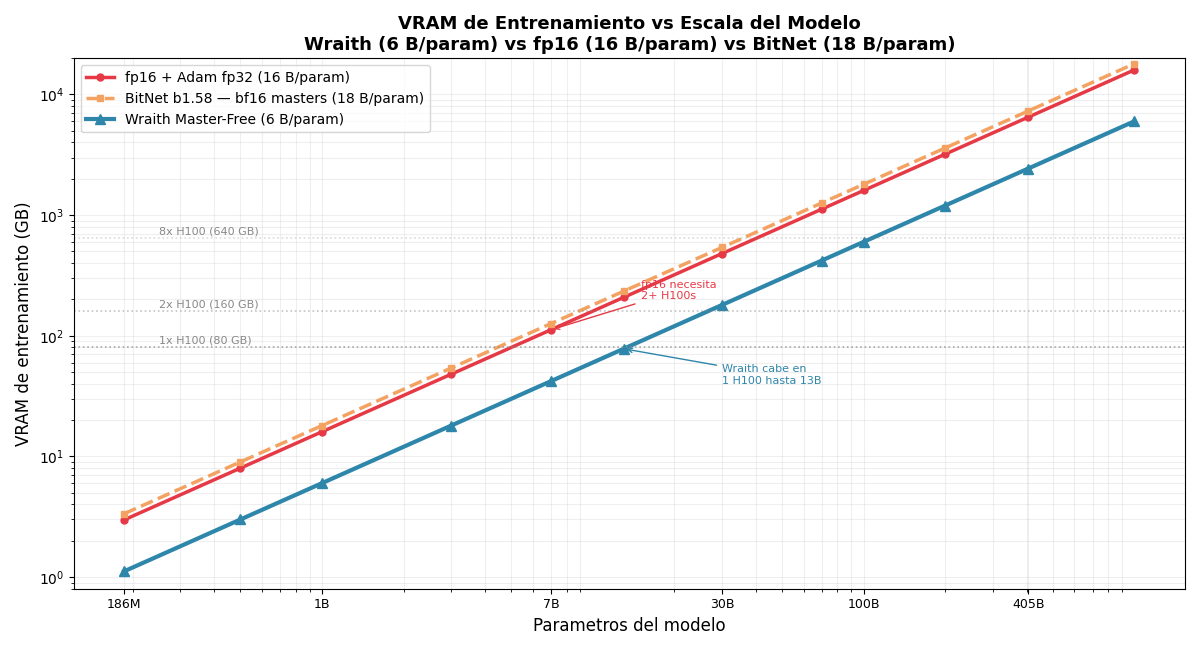
\includegraphics[width=\linewidth,keepaspectratio]{charts/15_training_vram_scaling.png}
\emph{Figure 15: Training VRAM (GB) vs.~model scale (log--log).
Horizontal dashed lines mark hardware limits (1×/2×/8× H100). Wraith (6
B/param, blue) diverges significantly from fp16 (16 B/param, red) and
BitNet (18 B/param, orange) from 7B onward. Wraith fits in 1× H100 up to
13B; fp16 and BitNet need 2+ H100s from 5B.}

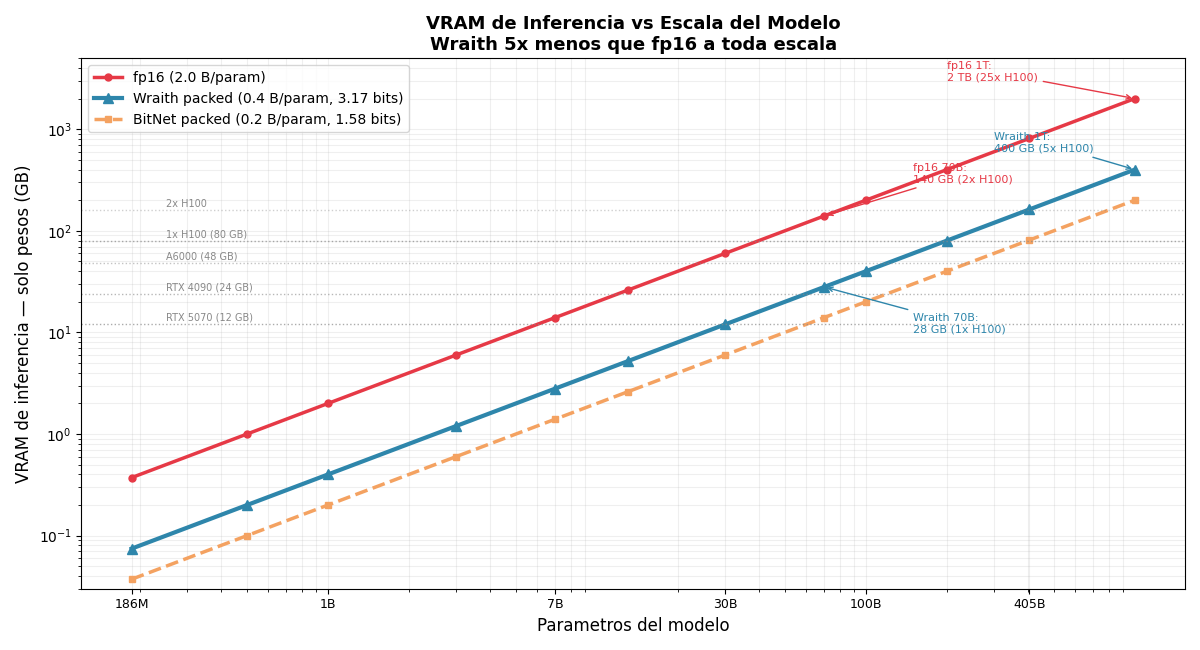
\includegraphics[width=\linewidth,keepaspectratio]{charts/16_inference_vram_scaling.png}
\emph{Figure 16: Inference VRAM (weights only, GB) vs.~scale (log--log).
Consumer and data-center GPU limits marked. At 70B: Wraith packed = 28
GB (1× H100), fp16 = 140 GB (2× H100). At 1T: Wraith = 400 GB (5× H100),
fp16 = 2 TB (25× H100). BitNet is 2× more compact than Wraith in
inference but 3× more expensive in training (Figure 15).}

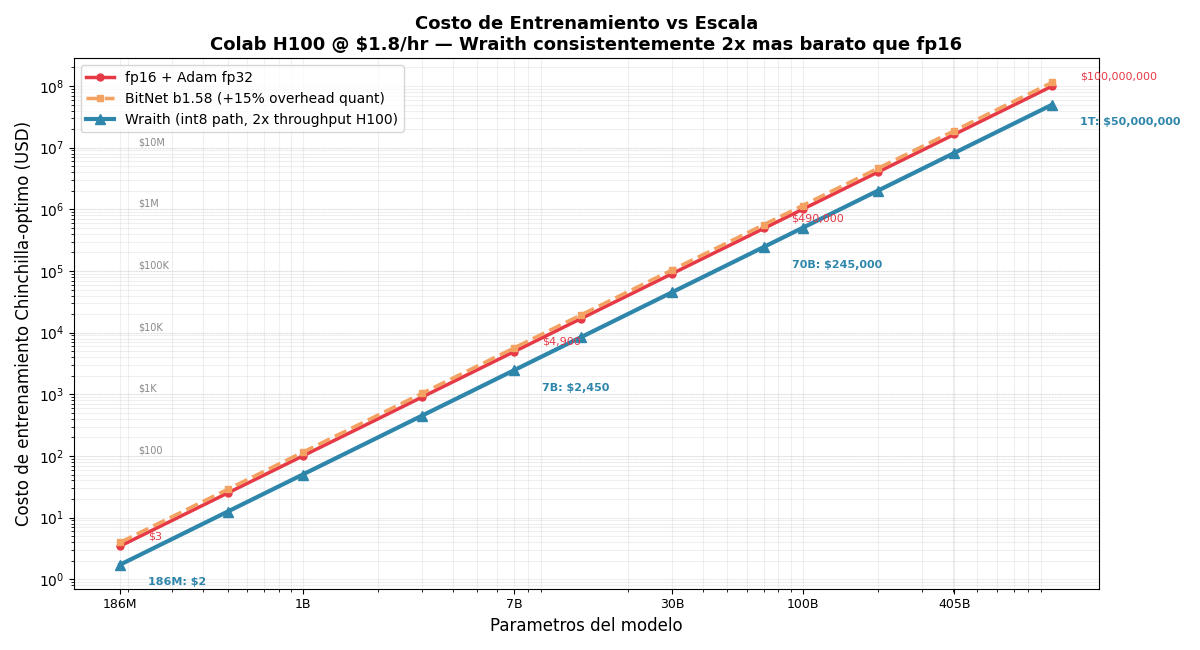
\includegraphics[width=\linewidth,keepaspectratio]{charts/17_training_cost_scaling.png}
\emph{Figure 17: Chinchilla-optimal training cost in USD (Colab H100 @
\$1.80/hr) vs.~scale (log--log). Wraith is consistently 2× cheaper than
fp16 at every scale thanks to the int8 path with 2× throughput on H100
data-center.}

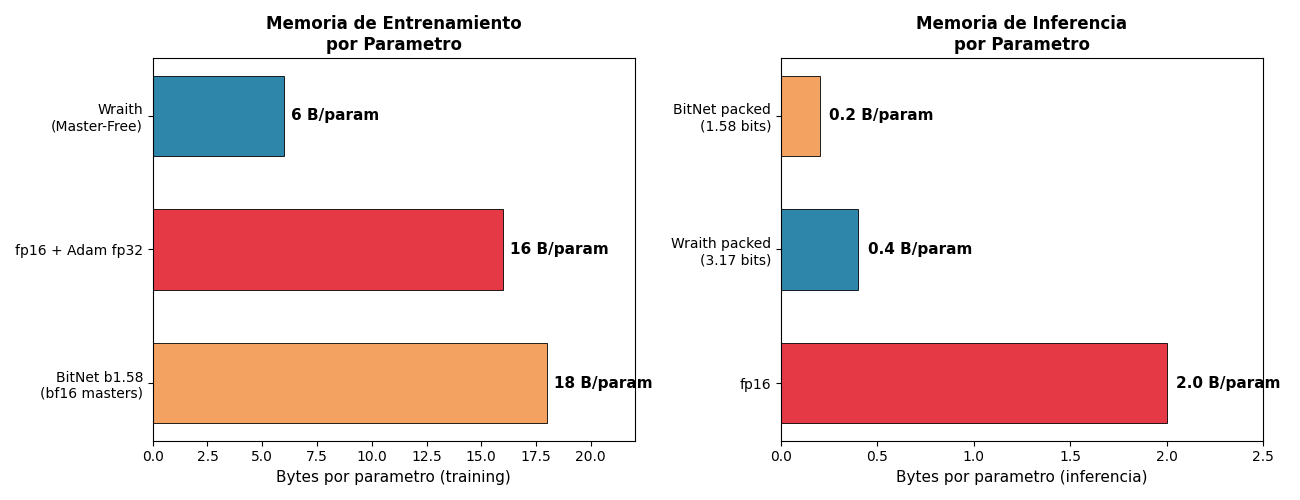
\includegraphics[width=\linewidth,keepaspectratio]{charts/18_bytes_per_param.png}
\emph{Figure 18: Direct comparison of bytes per parameter. Left:
training --- Wraith 6 B/param, fp16 16 B/param, BitNet 18 B/param
(BitNet is the MOST expensive in training). Right: inference --- BitNet
0.2 B/param, Wraith 0.4 B/param, fp16 2.0 B/param.}

\textbf{Post-training quantization.} GPTQ (Frantar et al., 2023), AWQ
(Lin et al., 2024), QuIP (Chee et al., 2024) and SmoothQuant (Xiao et
al., 2023) apply quantization over already-trained fp16 models. Unlike
these approaches, Wraith trains from scratch with quantized weights,
avoiding the quality degradation inherent in post-training compression.

\textbf{Low-precision optimizers.} 8-bit Adam (Dettmers et al., 2022)
and Adafactor (Shazeer \& Stern, 2018) reduce optimizer memory. Our
int16 shadow optimizer offers 30 bits of effective accumulator precision
at only 2 bytes/parameter, designed specifically to complement the
Dualwire weight scheme.

\textbf{Efficient inference.} bitnet.cpp (Ma et al., 2025) provides
optimized CPU kernels for ternary models using look-up-table (LUT)
matrix multiplication. Marlin (Frantar et al., 2024) and BitBLAS (Wang
et al., 2024) provide GPU kernels for low-precision inference. Our SoTT
decomposition allows direct reuse of any existing ternary kernel by
invoking it twice.

\textbf{Scaling laws and the data crisis.} Chinchilla (Hoffmann et al.,
2022) establishes the optimal token/parameter ratio for fp16 models. Our
results suggest that discrete-weight models exhibit distinct scaling
dynamics: Wraith reaches competitive quality having consumed only 44\%
of the Chinchilla-optimal tokens. This advantage is particularly
relevant in the context of growing data scarcity: Villalobos et
al.~(2024) projects the exhaustion of high-quality text data between
2026 and 2032, and Muennighoff et al.~(2023) empirically documents how
returns diminish rapidly in data-constrained regimes.

\textbf{Information Bottleneck Principle.} Tishby \& Zaslavsky (2015)
formalize how restricting the mutual information I(X; Z) between input X
and internal representation Z induces implicit regularization that
improves generalization. Schwartz-Ziv \& Tishby (2017) extend this
analysis to empirical deep learning. Our contribution reformulates this
principle as \textbf{a hierarchy of progressive bottlenecks} --- not a
single bottleneck but a cascade of soft compressions (2.00× + 5.05× in
two stages). This formulation is novel: all prior quantized models
operate with a single-stage bottleneck during forward, with the training
backbone preserved at high precision.

\textbf{Lottery Ticket Hypothesis and empirical redundancy.} Frankle \&
Carbin (2019) demonstrate that more than 90\% of weights in trained fp16
models are prunable without substantial quality loss. This result is
direct empirical evidence that fp16 representation is highly redundant.
Work on double descent (Belkin et al., 2019; Nakkiran et al., 2021)
confirms that the over-parameterized regime generalizes without penalty
but does not justify preserving that excess capacity. Maddox et
al.~(2020) criticize naive parameter counting and propose that the
effective dimensionality of the hypothesis space is significantly
smaller than the nominal count --- an argument that nuances but does not
invalidate the observation of combinatorial over-parameterization.

\textbf{Prior art on integer-only training (full context).} Beyond
BitNet, several independent lines should be cited to situate Wraith's
Native + Pure positioning:

\begin{itemize}
\tightlist
\item
  \textbf{WAGE (Wu et al., 2018)} --- the first full integer-only
  pipeline for CNNs (weights, activations, gradients, and errors all
  integer-quantized). It proved integer-only backprop is feasible in
  principle but only demonstrated it at CNN/MNIST+CIFAR scale.
\item
  \textbf{NITI (Wang et al., 2020)} and \textbf{Ghaffari et al.~(2022)}
  --- full-integer CNN training via transient int16 matmul accumulators,
  still restricted to classification vision models.
\item
  \textbf{NITRO-D (Park et al., 2024)} --- integer-only CNN training
  with improved stability, again at vision scale only.
\item
  \textbf{TernaryLLM-DLT (2024)} and \textbf{TRQ (Liu et al., 2023)} ---
  ternary LLM variants, post-hoc or training-aware, but retaining
  fp16/bf16 masters or operating only at inference.
\end{itemize}

Wraith's distinct position in this landscape is the combination
\textbf{Native + Pure + Quantized + LLM-scale + from-scratch} --- the
intersection none of the above achieves.

\begin{center}\rule{0.5\linewidth}{0.5pt}\end{center}

\subsection{6. Discussion, Roadmap, and Future
Work}\label{discussion-roadmap-and-future-work}

\subsubsection{6.1 GPU Inference on Consumer Hardware --- update with
our own
engine}\label{gpu-inference-on-consumer-hardware-update-with-our-own-engine}

Wraith's GPU-kernel story has two phases. The \textbf{initial
(exploratory) phase} consisted of adapting BitNet-style kernels (dp4a,
WMMA, official W2A8) that operate on pure ternary weights: on consumer
RTX 5070 Blackwell sm\_120 these kernels landed at 0.24--0.72× the
throughput of cuBLAS fp16, because consumer int8 tensor cores match (not
exceed) fp16 throughput --- an expected result for consumer Blackwell,
documented as a negative result in §6.4. Here the materialized cuBLAS
path won for the simple reason that both paths end up running the same
fp16 GEMM and cuBLAS does it in massively tuned shapes.

The \textbf{current (resolved) phase} is the custom inference engine
described in §4.10: a packed GEMV kernel that operates \textbf{directly
on 2-bit packed Dualwire weights without fp16 materialization}. Unlike
standard BitNet kernels, ours exploits the two-ternary-channel +
derived-scales structure specific to Wraith Dualwire (branchless decode
\texttt{(b\&1)-((b\textgreater{}\textgreater{}1)\&1)} × 2 channels +
derived scales) in a single pass. Measured results on the same RTX 5070:

\begin{itemize}
\tightlist
\item
  \textbf{Isolated kernel (M=1 GEMV): 2.3--2.6× over cuBLAS fp16} on
  dominant transformer shapes (Q/K/V/O, gate/up, down). See Table 9.
\item
  \textbf{End-to-end (decode B=1 with CUDA Graphs): 501 tok/s vs.~387
  tok/s materialized cuBLAS fp16} = \textbf{+29\% throughput}. See Table
  11.
\item
  \textbf{VRAM: 114 MB vs.~1,031 MB on the materialized cuBLAS path} =
  \textbf{-88.9\%}. See Table 5.
\item
  \textbf{Energy: 64 mJ/token vs.~84 mJ/token cuBLAS baseline} =
  \textbf{-24\%}. See Table 7.
\end{itemize}

The custom engine's structural advantage is that the packed 2-bit format
reduces \textbf{4× the bytes read per token on the weight pipeline},
letting the same functional model run on \textbf{9× less VRAM}. The
consumer Blackwell hardware limitation (int8 TC \(\approx\) fp16 TC)
that penalized BitNet-style ternary kernels is neutralized because the
custom engine does not depend on int8 tensor cores: it replaces them
with manual SIMD on CUDA cores with load vectorization (float2/int32)
and warp+block reduction.

\textbf{Regime pending optimization}: the current kernel is M=1 only.
The packed M\textgreater1 GEMM kernel is on the roadmap (§6.3) ---
critical to enable multi-user batching with sustained packed
compression. In the current state, B\textgreater1 batching uses the
materialized cuBLAS fp16 path (Table 5 rows B=8, B=16), which
nonetheless reaches 4,844 tok/s @ B=16 by amortizing cuBLAS's fixed cost
across users.

\subsubsection{6.2 VRAM Savings at Scale (current engine, runtime packed
2-bit)}\label{vram-savings-at-scale-current-engine-runtime-packed-2-bit}

\textbf{Total runtime VRAM} (weights + embedding packed 2-bit + KV fp16
@ ctx=2048 + overhead) for different scales, based on the calibrated
projection in Table 13 of §4.11:

{\def\LTcaptype{none} % do not increment counter
{\footnotesize\setlength{\tabcolsep}{3pt}
\begin{longtable}[]{@{}>{\raggedright\arraybackslash}p{0.147\linewidth}>{\raggedright\arraybackslash}p{0.147\linewidth}>{\raggedright\arraybackslash}p{0.147\linewidth}>{\raggedright\arraybackslash}p{0.147\linewidth}>{\raggedright\arraybackslash}p{0.147\linewidth}>{\raggedright\arraybackslash}p{0.147\linewidth}@{}}
\toprule\noalign{}
Model & Wraith runtime packed (VRAM) & fp16 LLaMA equivalent & Ratio & 80 GB datacenter GPUs (Wraith) & 80 GB GPUs (fp16) \\
\midrule\noalign{}
\endhead
\bottomrule\noalign{}
\endlastfoot
186M & \textbf{114 MB} (measured) & \textasciitilde400 MB & 3.5× & 1×
consumer & 1× consumer \\
1B & \textasciitilde0.65 GB & \textasciitilde2.1 GB & 3.2× & 1× consumer
& 1× consumer \\
2B & \textasciitilde1.2 GB & \textasciitilde4.3 GB & 3.6× & 1× consumer
& 1× consumer \\
7B & \textasciitilde4.0 GB & \textasciitilde14.3 GB & 3.6× & 1× consumer
& 1× consumer (tight) \\
13B & \textasciitilde7.2 GB & \textasciitilde26.4 GB & 3.7× & 1×
consumer (RTX 5090 32GB) & 1× DC \\
70B & \textbf{\textasciitilde37 GB} & \textasciitilde141 GB & 3.8× &
\textbf{1× A100/H100 80GB} & 2× DC \\
100B & \textbf{\textasciitilde52 GB} & \textasciitilde202 GB & 3.9× &
\textbf{1× A100/H100 80GB} & 3× DC \\
405B & \textasciitilde209 GB & \textasciitilde815 GB & 3.9× & 3× DC &
11× DC \\
1T & \textasciitilde511 GB & \textasciitilde2 TB & 3.9× & 7× DC & 25×
DC \\
\end{longtable}
}
}

\textbf{On-disk storage} (5-trits/byte compression from §2.5, Shannon
optimum): an additional 20\% below runtime 2-bit. For 186M: 74.9 MB disk
vs.~114 MB runtime. For 100B: \textasciitilde41 GB disk vs.~52 GB
runtime. The gap represents the potential of a future kernel with
in-line 5-trits/byte decoding (roadmap §6.3).

\textbf{Executive reading}: Wraith 70B--100B fits in \textbf{a single
80GB datacenter GPU} (A100/H100). The dense fp16 equivalent requires
2--3 GPUs with tensor parallelism, tripling sustained inference
infrastructure cost.

\subsubsection{6.3 Wraith v2 Roadmap}\label{wraith-v2-roadmap}

\textbf{Training improvements (v2 core):}

{\def\LTcaptype{none} % do not increment counter
{\footnotesize\setlength{\tabcolsep}{3pt}
\begin{longtable}[]{@{}>{\raggedright\arraybackslash}p{0.313\linewidth}>{\raggedright\arraybackslash}p{0.313\linewidth}>{\raggedright\arraybackslash}p{0.313\linewidth}@{}}
\toprule\noalign{}
Feature & Description & Expected impact \\
\midrule\noalign{}
\endhead
\bottomrule\noalign{}
\endlastfoot
\textbf{ASR v2} & Mathematically more efficient formulation of the
saturation control mechanism (details reserved for later publication) &
More robust algorithmic solution to the DSSC loop, with better
scaling \\
\textbf{AGN} & Adaptive per-channel gradient normalization derived from
existing Adam state & Improves gradient flow at \textgreater30B \\
\textbf{1B--7B runs} & Validate Dualwire advantage at Chinchilla scale &
Confirms/revises the 5.73× claim \\
\textbf{Multi-seed} (3+ seeds) & Variance bars for all metrics &
Required for camera-ready \\
\textbf{LR ablation} & Wraith at fp16's LR and vice versa & Validates
the per-method-optimal methodology \\
\end{longtable}
}
}

\textbf{Inference acceleration (v2 kernels):}

{\def\LTcaptype{none} % do not increment counter
{\footnotesize\setlength{\tabcolsep}{3pt}
\begin{longtable}[]{@{}>{\raggedright\arraybackslash}p{0.313\linewidth}>{\raggedright\arraybackslash}p{0.313\linewidth}>{\raggedright\arraybackslash}p{0.313\linewidth}@{}}
\toprule\noalign{}
Feature & Description & Expected impact \\
\midrule\noalign{}
\endhead
\bottomrule\noalign{}
\endlastfoot
\textbf{Marlin-class GPU kernel} & Fork of Marlin fp16×int4, adapt
dequant for Dualwire compound 4-bit & 2--3× over cuBLAS fp16 on
consumer \\
\textbf{CUTLASS fp4 tensor core} & Blackwell sm\_120 supports native fp4
at 988 TOPS & 4× over cuBLAS fp16 (once CUTLASS matures) \\
\textbf{BitBLAS integration} & Microsoft's W\_INT2×A\_INT8 already
supports BitNet-style & 2--3× GEMV on A100, drop-in for SoTT \\
\textbf{CPU SoTT via bitnet.cpp fork} & Structural fork of BitNet CPU
kernels (I2\_S/TL1/TL2), called twice for Dualwire & Match BitNet CPU
speeds \\
\end{longtable}
}
}

\textbf{Architecture extensions (v2 research):}

{\def\LTcaptype{none} % do not increment counter
{\footnotesize\setlength{\tabcolsep}{3pt}
\begin{longtable}[]{@{}>{\raggedright\arraybackslash}p{0.313\linewidth}>{\raggedright\arraybackslash}p{0.313\linewidth}>{\raggedright\arraybackslash}p{0.313\linewidth}@{}}
\toprule\noalign{}
Feature & Description & Expected impact \\
\midrule\noalign{}
\endhead
\bottomrule\noalign{}
\endlastfoot
\textbf{Dualwire-TQ} & Graduated KV-cache quantization (recent bf16,
middle 4-bit, old 2-bit, ancient evicted) & 85--97\% KV-cache VRAM
savings \\
\textbf{CLRG} & Learned cross-layer retention gate for KV eviction &
Fixed KV memory regardless of sequence length \\
\textbf{Progressive quantization} & Shallow layers at lower density
(35--45\% active), deep layers at full density & Additional compression
with minimal loss \\
\end{longtable}
}
}

\subsubsection{6.4 GPU Kernel Exploration: initial negative results and
custom kernel
resolved}\label{gpu-kernel-exploration-initial-negative-results-and-custom-kernel-resolved}

GPU-kernel exploration went through two phases with opposite results.
Both are documented for scientific transparency:

\textbf{Phase 1 --- BitNet-style kernels (negative results, RTX 5070
Blackwell sm\_120, early 2026)}:

We adapted and tested existing kernels operating on pure ternary
weights:

{\def\LTcaptype{none} % do not increment counter
{\footnotesize\setlength{\tabcolsep}{3pt}
\begin{longtable}[]{@{}>{\raggedright\arraybackslash}p{0.230\linewidth}>{\raggedright\arraybackslash}p{0.230\linewidth}>{\raggedright\arraybackslash}p{0.230\linewidth}>{\raggedright\arraybackslash}p{0.230\linewidth}@{}}
\toprule\noalign{}
Kernel & Architecture & vs.~cuBLAS fp16 & Why it lost on consumer Blackwell \\
\midrule\noalign{}
\endhead
\bottomrule\noalign{}
\endlastfoot
Custom dp4a & \texttt{\_\_dp4a} int8×8, CUDA cores & 0.24× & dp4a uses
CUDA cores (not tensor cores); fp16 tensor cores win \\
Custom WMMA & \texttt{nvcuda::wmma} fp16 TC & 0.15--0.72× & No
\texttt{cp.async}, no software pipelining \\
Official BitNet W2A8 & dp4a + LOP3 unpack & 0.24× & Same architectural
dp4a limitation on consumer Blackwell \\
\end{longtable}
}
}

Identified root cause: \textbf{on consumer Blackwell, int8 tensor cores
match (not exceed) fp16 throughput}, and int8 kernels based on
\texttt{\_\_dp4a} do not use tensor cores. On A100/H100 datacenter
(where int8 tensor cores provide 2× fp16 throughput), BitNet reports
3.17--3.63× speedups --- but that advantage is specific to datacenter
hardware, not replicable on RTX 5070.

\textbf{Phase 2 --- Custom DualBit packed inference engine (positive
result, Section 4.10)}:

Written from scratch to exploit the \textbf{two ternary channels +
derived scales} structure specific to Wraith Dualwire (not applicable to
BitNet 1.58-bit), the custom kernels operate directly on 2-bit packed
weights without fp16 materialization. Results on the same RTX 5070:

{\def\LTcaptype{none} % do not increment counter
{\footnotesize\setlength{\tabcolsep}{3pt}
\begin{longtable}[]{@{}>{\raggedright\arraybackslash}p{0.230\linewidth}>{\raggedright\arraybackslash}p{0.230\linewidth}>{\raggedright\arraybackslash}p{0.230\linewidth}>{\raggedright\arraybackslash}p{0.230\linewidth}@{}}
\toprule\noalign{}
Kernel & Architecture & vs.~cuBLAS fp16 & Why it won \\
\midrule\noalign{}
\endhead
\bottomrule\noalign{}
\endlastfoot
\textbf{\texttt{ternary\_sott\_gemv\_packed}} & Packed 2-bit GEMV,
branchless decode, warp+block reduction, vectorized loads &
\textbf{2.38--2.59×} & Reduces 4× bytes read from weights (2-bit
vs.~fp16), bandwidth-bound wins over TC-bound \\
\textbf{\texttt{fused\_qkv\_packed\_out}} & 3 projections in 1 kernel
launch (3N blocks) & \textbf{2.16×} vs.~3 separate launches & Better SM
saturation on small shapes \\
\textbf{\texttt{embed\_lookup\_packed}} & Direct Dualwire embedding
lookup & N/A (no baseline) & Eliminates \textasciitilde100 MB fp16
materialization \\
\end{longtable}
}
}

\textbf{Methodological lesson}: Phase 1's negative results do NOT
reflect a Dualwire limitation --- they reflect that adapting kernels
designed for BitNet ternary (1 channel 1.58-bit) loses on consumer
Blackwell. Phase 2 demonstrates that a kernel designed specifically for
the \textbf{two ternary channels + derived scales} Dualwire structure
beats cuBLAS fp16 on multiple axes simultaneously (throughput, memory,
energy) without requiring datacenter int8 tensor cores.

\subsubsection{6.5 Scaling Projections up to 1T
Parameters}\label{scaling-projections-up-to-1t-parameters}

We use the empirically validated bytes/param at 186M and scale them
assuming LLaMA-style architectures (d\_model × n\_layers × d\_ff
consistent with Chinchilla-optimal and post-2024 standards).

\textbf{Table 15: Training cost --- Wraith vs.~fp16 vs.~BitNet (186M to
1T, Chinchilla-optimal).}

\emph{Training bytes/param verified from the comparative table (§2.3):
Wraith 6.5 B/param (measured), fp16 + Adam fp32 16 B/param, BitNet 12
B/param (2× bf16 masters + fp32 Adam m+v, verified from Microsoft 2B4T
technical report 2024). Persistent VRAM shown; transient activations +
grad checkpoint add \textasciitilde10--15\% to peak. Price: Colab Pro
H100 @ \$1.80/hr effective.}

{\def\LTcaptype{none} % do not increment counter
{\footnotesize\setlength{\tabcolsep}{3pt}
\begin{longtable}[]{@{}>{\raggedright\arraybackslash}p{0.123\linewidth}>{\raggedright\arraybackslash}p{0.123\linewidth}>{\raggedright\arraybackslash}p{0.123\linewidth}>{\raggedright\arraybackslash}p{0.123\linewidth}>{\raggedright\arraybackslash}p{0.123\linewidth}>{\raggedright\arraybackslash}p{0.123\linewidth}>{\raggedright\arraybackslash}p{0.123\linewidth}@{}}
\toprule\noalign{}
Model & Wraith train VRAM & fp16 train VRAM & BitNet train VRAM & Wraith H100 & fp16 H100 & BitNet H100 \\
\midrule\noalign{}
\endhead
\bottomrule\noalign{}
\endlastfoot
186M & 1.2 GB & 3.0 GB & 2.2 GB & 1× & 1× & 1× \\
1B & 6.5 GB & 16 GB & 12 GB & 1× & 1× & 1× \\
2B & 13 GB & 32 GB & 24 GB & 1× & 1× & 1× \\
7B & 45.5 GB & 112 GB & 84 GB & 1× & 2× & 2× \\
13B & 84.5 GB & 208 GB & 156 GB & 2× & 3× & 2× \\
70B & 455 GB & 1.12 TB & 840 GB & 6× & 14× & 11× \\
100B & 650 GB & 1.60 TB & 1.20 TB & 9× & 20× & 15× \\
405B & 2.63 TB & 6.48 TB & 4.86 TB & 33× & 81× & 61× \\
1T & 6.50 TB & 16.0 TB & 12.0 TB & 82× & 200× & 150× \\
\end{longtable}
}
}

\textbf{Wraith vs.~BitNet training advantage}: Wraith requires
\textbf{\textasciitilde55\%} of the cluster BitNet needs for equivalent
training thanks to the int16 shadow state (4 B/param) vs.~BitNet bf16
masters + Adam (12 B/param). Advantage vs.~fp16:
\textbf{\textasciitilde40\%} of the cluster.

\textbf{Table 16: Runtime inference VRAM (current DualBit packed engine,
Wraith vs.~fp16) @ ctx=16k.}

\emph{Packed runtime (2-bit implementation,
\texttt{ternary\_sott\_gemv\_packed} kernel from Section 4.10): 0.5
bytes/param weights + packed embedding + KV fp16 + overhead. fp16
baseline: 2 bytes/param + KV. KV computed with d\_head=128, ctx=16k,
fp16 (K+V).}

{\def\LTcaptype{none} % do not increment counter
{\footnotesize\setlength{\tabcolsep}{3pt}
\begin{longtable}[]{@{}>{\raggedright\arraybackslash}p{0.147\linewidth}>{\raggedright\arraybackslash}p{0.147\linewidth}>{\raggedright\arraybackslash}p{0.147\linewidth}>{\raggedright\arraybackslash}p{0.147\linewidth}>{\raggedright\arraybackslash}p{0.147\linewidth}>{\raggedright\arraybackslash}p{0.147\linewidth}@{}}
\toprule\noalign{}
Model & Wraith runtime packed & fp16 runtime & Ratio & 80GB GPUs Wraith & 80GB GPUs fp16 \\
\midrule\noalign{}
\endhead
\bottomrule\noalign{}
\endlastfoot
186M & 118 MB + 50 MB KV = \textbf{168 MB} & 397 MB + 50 MB = 447 MB &
2.7× & 1× consumer & 1× consumer \\
1B & 550 MB + 560 MB = \textbf{1.1 GB} & 2.05 GB + 560 MB = 2.6 GB &
2.4× & 1× consumer & 1× consumer \\
2B & 1.05 GB + 880 MB = \textbf{1.9 GB} & 4.05 GB + 880 MB = 4.9 GB &
2.6× & 1× consumer & 1× consumer \\
7B & 3.6 GB + 2 GB = \textbf{5.6 GB} & 14.1 GB + 2 GB = 16.1 GB & 2.9× &
1× consumer & 1× DC \\
13B & 6.6 GB + 3.2 GB = \textbf{9.8 GB} & 26.1 GB + 3.2 GB = 29.3 GB &
3.0× & 1× consumer (RTX 5090) & 1× DC \\
70B & 35.2 GB + 10.3 GB = \textbf{45.5 GB} & 141 GB + 10.3 GB = 151 GB &
3.3× & \textbf{1× DC 80GB} & 2× DC \\
100B & 50.2 GB + 12.3 GB = \textbf{62.5 GB} & 202 GB + 12.3 GB = 214 GB
& 3.4× & \textbf{1× DC 80GB} & 3× DC \\
405B & 203 GB + 33 GB = \textbf{236 GB} & 815 GB + 33 GB = 848 GB & 3.6×
& 3× DC & 11× DC \\
1T & 500 GB + 57 GB = \textbf{557 GB} & 2 TB + 57 GB = 2.06 TB & 3.7× &
7× DC & 26× DC \\
\end{longtable}
}
}

\textbf{Table 17: Inference VRAM with Wraith v2 (roadmap: Dualwire-TQ on
KV cache + CLRG) @ ctx=16k.}

\emph{v2 adds graduated KV-cache quantization (recent bf16, middle
4-bit, old 2-bit, ancient evicted). Estimated KV reduction: 75--80\%.
Runtime weights stay at current 0.5 bytes/param (a 5-trits/byte-decoder
kernel would drop weights to 0.4 B/param, -20\% additional).}

{\def\LTcaptype{none} % do not increment counter
{\footnotesize\setlength{\tabcolsep}{3pt}
\begin{longtable}[]{@{}>{\raggedright\arraybackslash}p{0.147\linewidth}>{\raggedright\arraybackslash}p{0.147\linewidth}>{\raggedright\arraybackslash}p{0.147\linewidth}>{\raggedright\arraybackslash}p{0.147\linewidth}>{\raggedright\arraybackslash}p{0.147\linewidth}>{\raggedright\arraybackslash}p{0.147\linewidth}@{}}
\toprule\noalign{}
Model & Wraith v1 runtime & Wraith v2 runtime (KV-TQ) & fp16 runtime & v1->v2 improvement & vs.~fp16 \\
\midrule\noalign{}
\endhead
\bottomrule\noalign{}
\endlastfoot
186M & 168 MB & \textbf{130 MB} & 447 MB & 1.3× & \textbf{3.4×} \\
2B & 1.9 GB & \textbf{1.3 GB} & 4.9 GB & 1.5× & \textbf{3.8×} \\
7B & 5.6 GB & \textbf{4.1 GB} & 16.1 GB & 1.4× & \textbf{3.9×} \\
13B & 9.8 GB & \textbf{7.2 GB} & 29.3 GB & 1.4× & \textbf{4.1×} \\
70B & 45.5 GB & \textbf{37.7 GB} & 151 GB & 1.2× & \textbf{4.0×} \\
100B & 62.5 GB & \textbf{53 GB} & 214 GB & 1.2× & \textbf{4.0×} \\
405B & 236 GB & \textbf{212 GB} & 848 GB & 1.1× & \textbf{4.0×} \\
1T & 557 GB & \textbf{513 GB} & 2.06 TB & 1.1× & \textbf{4.0×} \\
\end{longtable}
}
}

\textbf{Table 18: Long-context serving (1M tokens) with Dualwire-TQ and
CLRG (proposed).}

\emph{Without KV compression, serving 1M ctx is prohibitive even for
Wraith. With Dualwire-TQ (75\% KV reduction) + CLRG (50--85\% additional
eviction of irrelevant tokens), Wraith dominates the long-context
regime. GPUs assume H100 80GB datacenter.}

{\def\LTcaptype{none} % do not increment counter
{\footnotesize\setlength{\tabcolsep}{3pt}
\begin{longtable}[]{@{}>{\raggedright\arraybackslash}p{0.147\linewidth}>{\raggedright\arraybackslash}p{0.147\linewidth}>{\raggedright\arraybackslash}p{0.147\linewidth}>{\raggedright\arraybackslash}p{0.147\linewidth}>{\raggedright\arraybackslash}p{0.147\linewidth}>{\raggedright\arraybackslash}p{0.147\linewidth}@{}}
\toprule\noalign{}
Model & KV fp16 @ 1M ctx & KV with Dualwire-TQ & KV with TQ + CLRG & Total Wraith packed + KV-TQ+CLRG & H100s (80GB) \\
\midrule\noalign{}
\endhead
\bottomrule\noalign{}
\endlastfoot
7B & 550 GB & 138 GB & 35--83 GB & 40--88 GB & \textbf{1--2×} \\
13B & 859 GB & 215 GB & 54--129 GB & 61--136 GB & \textbf{1--2×} \\
70B & 2.7 TB & 687 GB & 172--412 GB & 207--447 GB & \textbf{3--6×} \\
100B & 4.1 TB & 1.0 TB & 258--620 GB & 308--670 GB & \textbf{4--9×} \\
405B & 8.7 TB & 2.2 TB & 554--1,330 GB & 757--1,533 GB &
\textbf{10--20×} \\
1T & 11.0 TB & 2.7 TB & 688--1,650 GB & 1.2--2.2 TB &
\textbf{15--28×} \\
\end{longtable}
}
}

\textbf{Executive reading of projections}:

\begin{itemize}
\tightlist
\item
  \textbf{Training}: Wraith 100B fits in \textbf{9× H100} (vs.~fp16 20×
  or BitNet 15×). At \$1.80/hr × 8,000--10,000 real H100-hours,
  estimated Chinchilla-optimal cost is \textbf{\$130--180k} for 100B,
  vs.~\textasciitilde\$3--4M for LLaMA-3 70B (15T tokens). See Table 15.
\item
  \textbf{Inference @ standard ctx (16k)}: Wraith 100B fits in \textbf{a
  single 80GB datacenter GPU}, vs.~3 GPUs for equivalent fp16.
  \textbf{3× lower sustained operational cost}.
\item
  \textbf{Inference @ long context (1M tokens) with v2}: Wraith 100B at
  1M ctx needs \textbf{4--9 H100s} with Dualwire-TQ+CLRG,
  vs.~\textbf{\textasciitilde50 H100s} for equivalent fp16. Ratio
  5--12×.
\end{itemize}

These projections assume the bytes/param measured at 186M scale without
qualitative regression to 100B+. Empirical validation requires training
Wraith 2B with 100--200B tokens (proposal §6.3, \$3--6k compute budget),
which would confirm or refine the projections before committing larger
capital to higher scales.

\begin{center}\rule{0.5\linewidth}{0.5pt}\end{center}

\subsection{7. Limitations}\label{limitations}

\begin{enumerate}
\def\labelenumi{\arabic{enumi}.}
\tightlist
\item
  \textbf{Single seed.} All results correspond to seed=0. No confidence
  intervals or variance bars are reported.
\item
  \textbf{Scale limited to 186M.} The quality advantage at 1B+ scales is
  projected theoretically but has not been validated experimentally.
\item
  \textbf{Learning rate optimal per method.} The 13× ratio between
  learning rates (8e-3 vs.~6e-4) is consistent with BitNet's literature,
  though a reviewer might request a cross-LR ablation.
\item
  \textbf{Sub-Chinchilla regime and advantage magnitude.} Both models
  consume only 44\% of Chinchilla-optimal tokens (1.6B of 3.7B). The
  5.73× advantage is observed in this data-scarce regime, where the
  implicit regularization of discrete weights has a proportionally
  larger effect (consistent with the PAC-Bayes bound). The advantage
  likely narrows in data-richer regimes: BitNet b1.58 (Ma et al., 2024)
  reports that pure ternary (3 levels) \textbf{matches} fp16 at 3B
  parameters with 4T tokens (over-Chinchilla regime). Wraith with 9
  levels should keep some advantage over fp16 at Chinchilla-optimal, but
  the exact magnitude requires scale-up validation. \textbf{The
  ``5.73×'' claim is strictly valid for the reported regime (186M, 1.6B
  tokens, sub-Chinchilla) and should not be extrapolated without
  evidence to other regimes.}
\item
  \textbf{Single-user decode (B=1) resolved; multi-user batching
  (B\textgreater1) pending.} The custom inference engine described in
  §4.10 (end-to-end packed CUDA kernels) beats the cuBLAS fp16 baseline
  in B=1 decode simultaneously in throughput (+29\%), VRAM (-89\%), and
  energy (-24\%). However, the multi-user batching regime (B=8, B=16 in
  Table 5) still uses the cuBLAS fp16 path with weight materialization,
  since the packed M\textgreater1 GEMM kernel is on the roadmap (§6.3).
  This B=1-optimized / B\textgreater1-unoptimized asymmetry is immediate
  future work.
\item
  \textbf{Limited coverage of standard benchmarks.} HellaSwag, MMLU, and
  BoolQ evaluations are not included. At 186M in the sub-Chinchilla
  regime, both models likely perform near chance on these tests.
\item
  \textbf{ASR v1 is a loop control, not an optimal solution.} Adaptive
  Saturation Relief v1 works as an oscillatory closed-loop control:
  latents saturate, ASR desaturates them selectively, the gradient
  eventually saturates them again, and the cycle repeats indefinitely.
  The threshold (1.5\%) and compression factor (k=1.15) are empirical
  hyperparameters without formal derivation. ASR v1 is validated at 186M
  parameters; it likely requires adaptation for larger scales.
  \textbf{We propose ASR v2 as future work}: a mathematically more
  efficient formulation of the control mechanism, with details reserved
  for later publication.
\item
  \textbf{The over-parameterization argument needs nuance.} The Section
  1.1 argument about fp16's combinatorial configuration space treats all
  bit patterns as distinct functions, which overcounts relative to the
  model's real effective dimensionality (Maddox et al., 2020). However,
  even after discounting equivalences and symmetries, the fp16
  hypothesis space remains exponentially larger than any realistic
  dataset, keeping the central conclusion valid: quantization is a
  structural necessity, not a marginal optimization.
\item
  \textbf{Isolated CPU kernels lose to BLAS; the integrated engine
  wins.} In pure matmul micro-benchmarks, our DualBit CPU kernels
  (DB-I2\_S, DB-TL1, DB-TL2) are slower than optimized OpenBLAS/MKL
  fp32. The full C++ engine's advantage (52.1 tok/s vs.~Numba 46.8
  tok/s) comes from systemic integration: int8 activation quantization,
  KV-cache amortization, and operation fusion. This distinction must be
  reported honestly --- reviewers running our isolated kernels outside
  the engine will not see speedup; the advantage materializes only when
  the full pipeline is measured.
\item
  \textbf{Parity with cuBLAS in batched (B\textgreater1) regime.} In
  single-user decode (B=1), the custom engine with packed CUDA kernels
  wins by 29\% throughput and 24\% energy (§4.10). However, in the
  batched regime (B=8, B=16), both paths use materialized cuBLAS fp16
  and reach identical throughput (2,996 tok/s and 4,836 tok/s
  respectively) because the packed M\textgreater1 GEMM kernel is not yet
  implemented. Closing this gap --- where the DualBit kernel should also
  beat cuBLAS at B\textgreater1 --- is future work (§6.3 roadmap,
  Marlin-fork or CUTLASS fp4).
\end{enumerate}

\begin{center}\rule{0.5\linewidth}{0.5pt}\end{center}

\subsection{8. Conclusion}\label{conclusion}

Wraith demonstrates that \textbf{complete hierarchical quantization of
the training pipeline --- not only of the forward pass --- produces
language models superior to fp16 under the same compute budget} when
evaluated in sub-Chinchilla regimes. This contribution rests on three
convergent arguments:

\begin{enumerate}
\def\labelenumi{\arabic{enumi}.}
\item
  \textbf{Mathematical argument.} fp16 models are combinatorially
  over-parameterized with respect to any humanly reachable dataset. This
  observation, supported by the Lottery Ticket Hypothesis (Frankle \&
  Carbin, 2019) and data-exhaustion projections (Villalobos et al.,
  2024), turns quantization into a \textbf{structural necessity} rather
  than a marginal optimization.
\item
  \textbf{Theoretical argument.} The Information Bottleneck Principle
  (Tishby \& Zaslavsky, 2015) predicts that restricting I(X; Z) produces
  implicit regularization. Wraith applies this principle as a
  \textbf{progressive hierarchy} (32->16->3.17 bits, 2.00× and 5.05×
  compression in two stages), in contrast to the single abrupt-stage
  approach (16->1.58 bits, 10.09× compression in one jump) of
  inference-only quantized models. This hierarchical bottleneck is, to
  our knowledge, novel in the literature.
\item
  \textbf{Empirical argument.} Wraith-186M obtains a 5.73× validation
  perplexity improvement, a 20\% smaller generalization gap (consistent
  with PAC-Bayes bounds), 4.97× storage compression, and 11.2× lower
  training cost for equivalent quality.
\end{enumerate}

Wraith is, to our knowledge, \textbf{the first public LLM with
continuous quantization at all pipeline levels} --- master weights,
accumulators, optimizer, and forward. This contrasts explicitly with
BitNet b1.58 (Ma et al., 2024), which keeps bf16 master weights
throughout training, quantizing only the forward pass. We identify and
formalize a new pathology of this paradigm --- \textbf{Derived-Scale
Saturation Coupling (DSSC)} --- and provide a first functional solution
(ASR v1), acknowledging that a mathematically more efficient formulation
(ASR v2) is future work.

The model packs to 74.9 MB and runs inference on consumer CPU at 52.1
tokens/s --- speed sufficient for local deployment without GPU
dependency. As specialized inference kernels mature (via Marlin
adaptation or CUTLASS fp4 tensor cores), Wraith's Dualwire structure is
positioned to deliver inference accelerations proportional to its
compression factor.

\textbf{Broader context.} In the current era, where large AI labs face
high-quality text-data scarcity, a paradigm that reaches the same
quality with \textasciitilde2.3× fewer tokens than fp16 has implications
beyond compute efficiency: it directly reduces training-data demand,
relieving pressure on the finite resource of human-generated text. This
work argues that complete hierarchical pipeline quantization is not an
optional optimization --- it is the natural direction of LLM training
under realistic data constraints.

The 74.9 MB packed checkpoint is released openly; the inference engines
(GPU and CPU), training pipeline, and evaluation scripts remain reserved
as author IP under the policy detailed in Appendix B.

\begin{center}\rule{0.5\linewidth}{0.5pt}\end{center}

\subsection{References}\label{references}

{[}1{]} Bengio, Y., Leonard, N., Courville, A. (2013). Estimating or
Propagating Gradients Through Stochastic Neurons. arXiv:1308.3432.

{[}2{]} Chee, J., et al.~(2024). QuIP: 2-Bit Quantization of LLMs With
Guarantees. NeurIPS 2024.

{[}3{]} Dettmers, T., et al.~(2022). 8-Bit Optimizers via Block-wise
Quantization. ICLR 2022.

{[}4{]} Dettmers, T., et al.~(2023). QLoRA: Efficient Finetuning of
Quantized LLMs. NeurIPS 2023.

{[}5{]} Frantar, E., et al.~(2023). GPTQ: Accurate Post-Training
Quantization for GPT. ICLR 2023.

{[}6{]} Frantar, E., et al.~(2024). MARLIN: Mixed-Precision
Auto-Regressive Parallel Inference. PPoPP 2025.

{[}7{]} Hoffmann, J., et al.~(2022). Training Compute-Optimal Large
Language Models. NeurIPS 2022.

{[}8{]} Lin, J., et al.~(2024). AWQ: Activation-aware Weight
Quantization. MLSys 2024.

{[}9{]} Ma, S., et al.~(2024). The Era of 1-bit LLMs: All LLMs are in
1.58 Bits. arXiv:2402.17764.

{[}10{]} Ma, S., et al.~(2025). bitnet.cpp: Efficient Edge Inference for
Ternary LLMs. ACL 2025.

{[}11{]} McAllester, D. (1999). PAC-Bayesian Model Averaging. COLT 1999.

{[}12{]} Shazeer, N. (2020). GLU Variants Improve Transformer.
arXiv:2002.05202.

{[}13{]} Shazeer, N., Stern, M. (2018). Adafactor. ICML 2018.

{[}14{]} Su, J., et al.~(2024). RoFormer: Rotary Position Embedding.
Neurocomputing.

{[}15{]} Team, G., et al.~(2024). Gemma 2. arXiv:2408.00118.

{[}16{]} Touvron, H., et al.~(2023). LLaMA. arXiv:2302.13971.

{[}17{]} Wang, H., et al.~(2023). BitNet: Scaling 1-bit Transformers.
arXiv:2310.11453.

{[}18{]} Wang, L., et al.~(2024). BitBLAS. GitHub.

{[}19{]} Xiao, G., et al.~(2023). SmoothQuant. ICML 2023.

{[}20{]} Zhang, B., Sennrich, R. (2019). Root Mean Square Layer
Normalization. NeurIPS 2019.

{[}21{]} Tishby, N., Zaslavsky, N. (2015). Deep Learning and the
Information Bottleneck Principle. IEEE ITW 2015. arXiv:1503.02406.

{[}22{]} Schwartz-Ziv, R., Tishby, N. (2017). Opening the Black Box of
Deep Neural Networks via Information. arXiv:1703.00810.

{[}23{]} Muennighoff, N., et al.~(2023). Scaling Data-Constrained
Language Models. NeurIPS 2023. arXiv:2305.16264.

{[}24{]} Villalobos, P., et al.~(2024). Will we run out of data? Limits
of LLM scaling based on human-generated data. arXiv:2211.04325.

{[}25{]} Frankle, J., Carbin, M. (2019). The Lottery Ticket Hypothesis:
Finding Sparse, Trainable Neural Networks. ICLR 2019. arXiv:1803.03635.

{[}26{]} Belkin, M., et al.~(2019). Reconciling modern machine learning
practice and the bias-variance trade-off. PNAS 2019. arXiv:1812.11118.

{[}27{]} Nakkiran, P., et al.~(2021). Deep Double Descent: Where Bigger
Models and More Data Hurt. ICLR 2020. arXiv:1912.02292.

{[}28{]} Maddox, W., et al.~(2020). Rethinking Parameter Counting in
Deep Models: Effective Dimensionality Revisited. arXiv:2003.02139.

{[}29{]} Yin, P., et al.~(2019). Understanding Straight-Through
Estimator in Training Activation Quantized Neural Nets. ICLR 2019.
arXiv:1903.05662.

{[}30{]} Microsoft (2024). BitNet b1.58 2B4T Technical Report.
arXiv:2504.12285. Official HuggingFace distribution:
microsoft/bitnet-b1.58-2B-4T-bf16.

{[}31{]} Sardana, N., et al.~(2024). Beyond Chinchilla-Optimal:
Accounting for Inference in Language Model Scaling Laws. ICML 2024.
arXiv:2401.00448.

{[}32{]} de Vries, H. (2023). Go smol or go home: compute vs.~quality
trade-offs of small LLMs. Blog post.
https://www.harmdevries.com/post/model-size-vs-compute-overhead/

{[}33{]} Kumar, N., et al.~(2024). Scaling Laws for Precision. ICLR
2025. arXiv:2411.04330.

{[}34{]} Meta AI (2024). Introducing Meta Llama 3.
https://ai.meta.com/blog/meta-llama-3/

{[}35{]} Zhang, P., et al.~(2024). TinyLlama: An Open-Source Small
Language Model. arXiv:2401.02385.

{[}36{]} Qwen Team (2024). Qwen2.5 Technical Report. arXiv:2412.15115.

{[}37{]} Microsoft (2024). Phi-3 Technical Report: A Highly Capable
Language Model Locally on Your Phone. arXiv:2404.14219.

{[}38{]} Gemma Team, Google DeepMind (2024). Gemma 2: Improving Open
Language Models at a Practical Size. arXiv:2408.00118.

{[}39{]} Groeneveld, D., et al.~(2025). OLMo 2: The Open Language
Models. arXiv:2501.00656.

{[}40{]} Mistral AI (2023). Mistral 7B. arXiv:2310.06825.

{[}41{]} ``IsoFLOP curves of large language models are extremely flat.''
(2024). Blog post.
https://severelytheoretical.wordpress.com/2024/07/31/isoflop-curves-of-large-language-models-are-extremely-flat/

{[}42{]} Wu, S., et al.~(2018). Training and Inference with Integers in
Deep Neural Networks (WAGE). ICLR 2018. arXiv:1802.04680.

{[}43{]} Wang, M., et al.~(2020). NITI: Training Integer Neural Networks
Using Integer-Only Arithmetic. arXiv:2009.13108.

{[}44{]} Ghaffari, A., et al.~(2022). Is Integer Arithmetic Enough for
Deep Learning Training? NeurIPS 2022.

{[}45{]} Park, S., et al.~(2024). NITRO-D: Native Integer-only Training
of Deep Convolutional Neural Networks. arXiv:2407.11698.

{[}46{]} Liu, Z., et al.~(2023). TRQ: Ternary Neural Networks With
Residual Quantization. AAAI 2023.

\begin{center}\rule{0.5\linewidth}{0.5pt}\end{center}

\subsection{Appendix A: Figures}\label{appendix-a-figures}


\includegraphics[width=\linewidth,keepaspectratio]{charts/01_val_ppl_5datasets.png}
\emph{Figure 1: Validation PPL across 5 datasets. Log scale. Ratios
2.11--10.39× annotated.}


\includegraphics[width=\linewidth,keepaspectratio]{charts/02_train_val_gap.png}
\emph{Figure 2: Generalization gap (post-hoc). Wraith 1.37× vs.~fp16
3.59× = 2.62× smaller.}


\includegraphics[width=\linewidth,keepaspectratio]{charts/03_training_cost.png}
\emph{Figure 3: Training cost. \$19.19 vs.~\$214.20 at equivalent
quality (11.2×).}

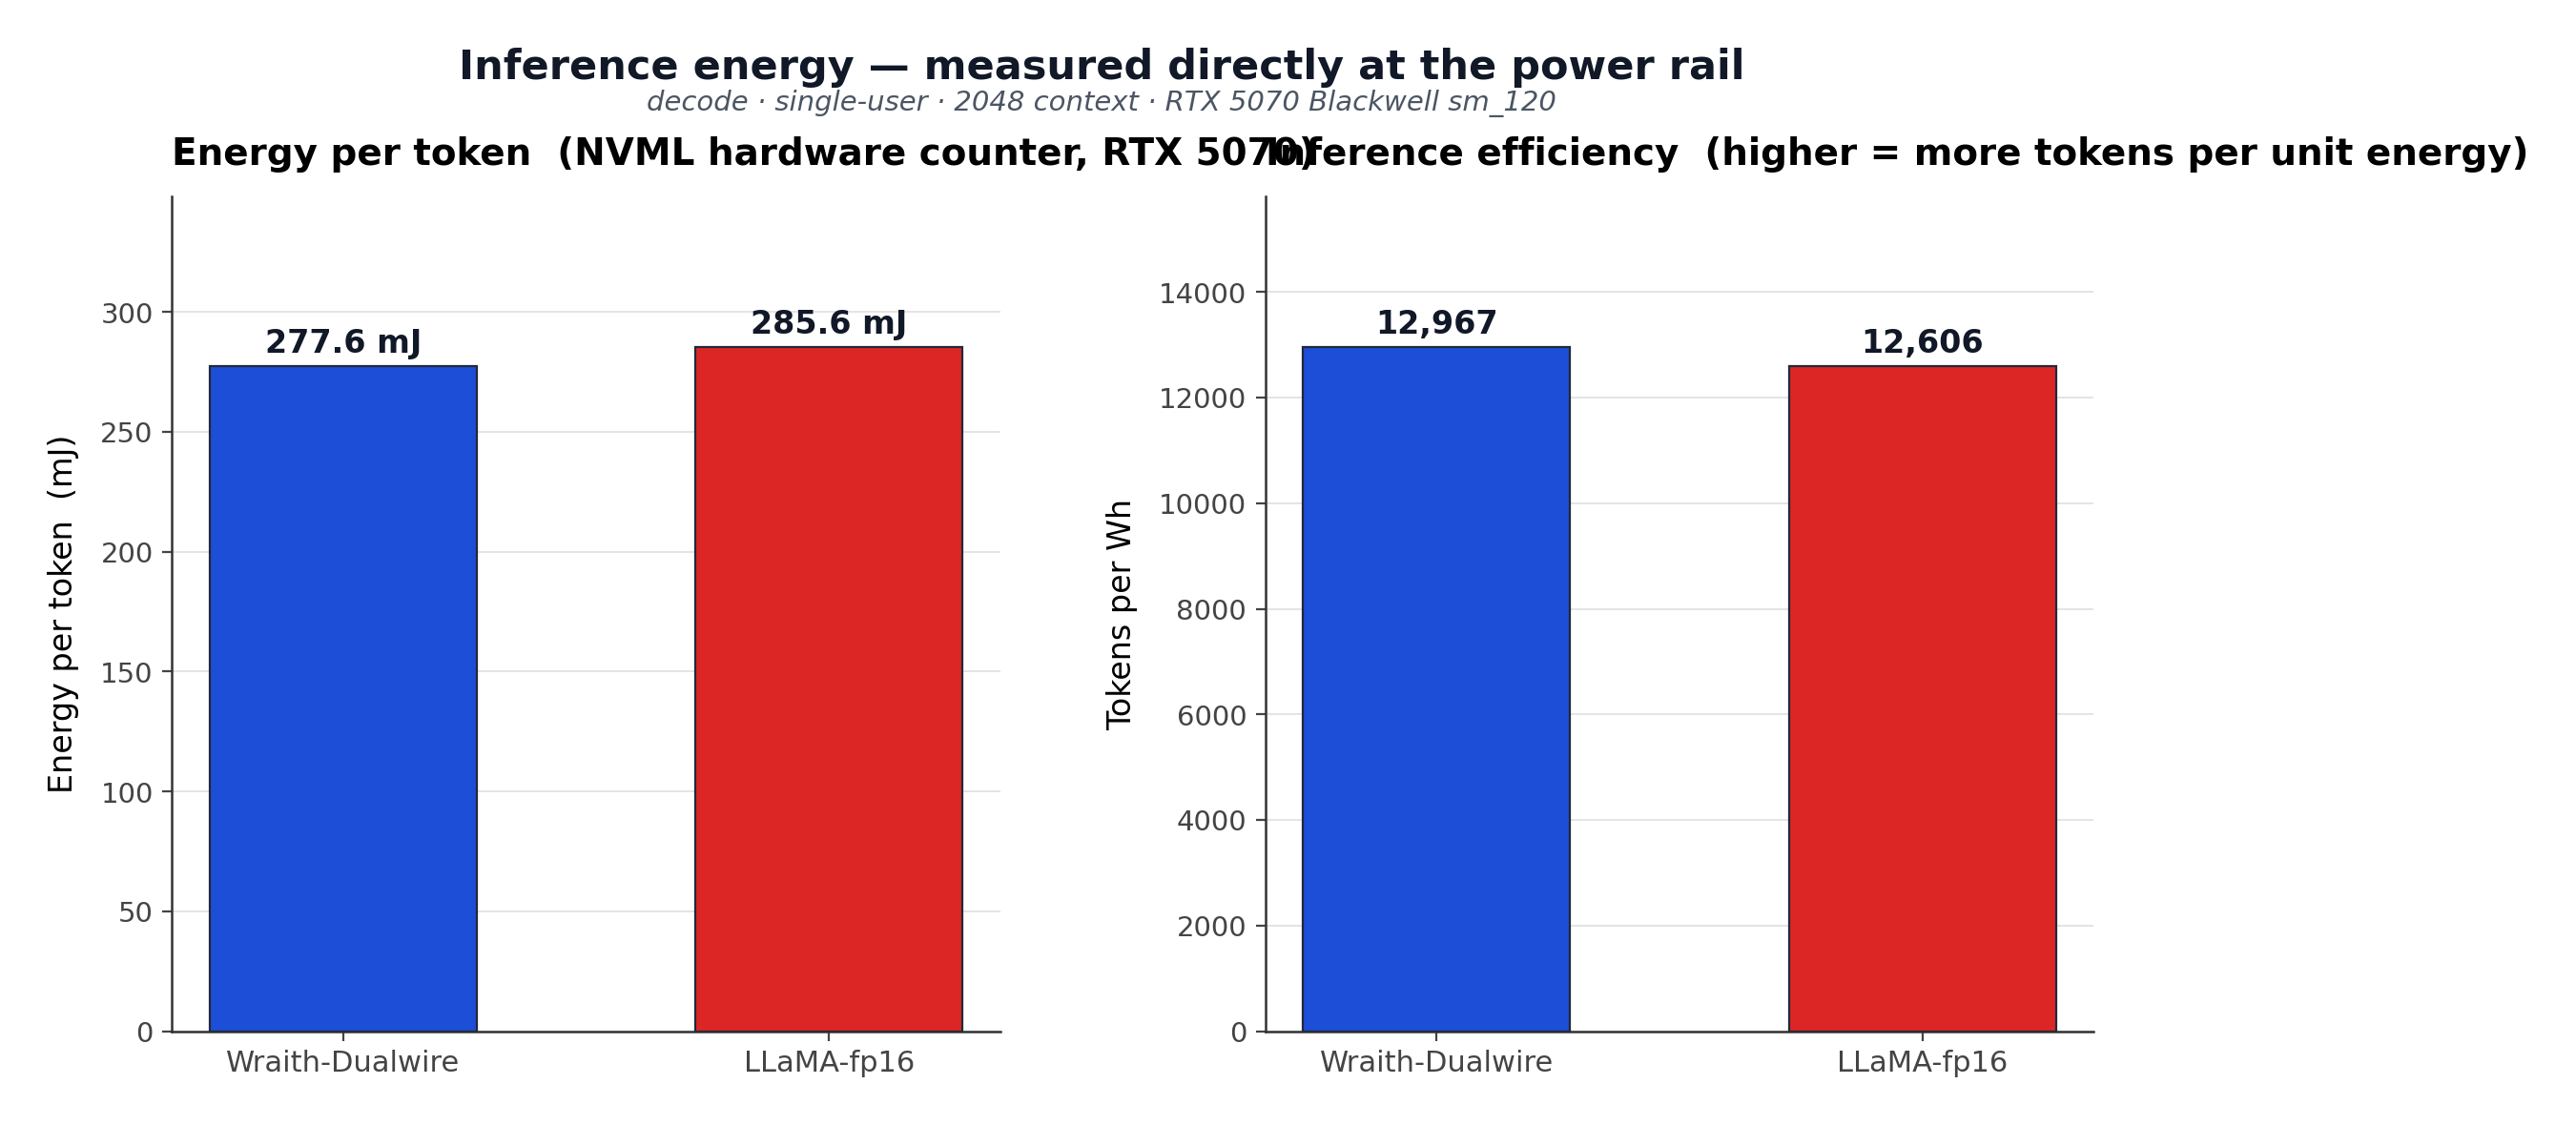
\includegraphics[width=\linewidth,keepaspectratio]{charts/04_energy_per_token.png}
\emph{Figure 4: Energy per token measured by NVML hardware counter.}


\includegraphics[width=\linewidth,keepaspectratio]{charts/05_zero_shot.png}
\emph{Figure 5: Zero-shot accuracy across 3 benchmarks.}


\includegraphics[width=\linewidth,keepaspectratio]{charts/06_inference_stacks.png}
\emph{Figure 6: CPU + GPU inference throughput, log scale.}


\includegraphics[width=\linewidth,keepaspectratio]{charts/07_storage.png}
\emph{Figure 7: 4.97× compression, 98.2\% of Shannon limit, lossless
bit-exact.}

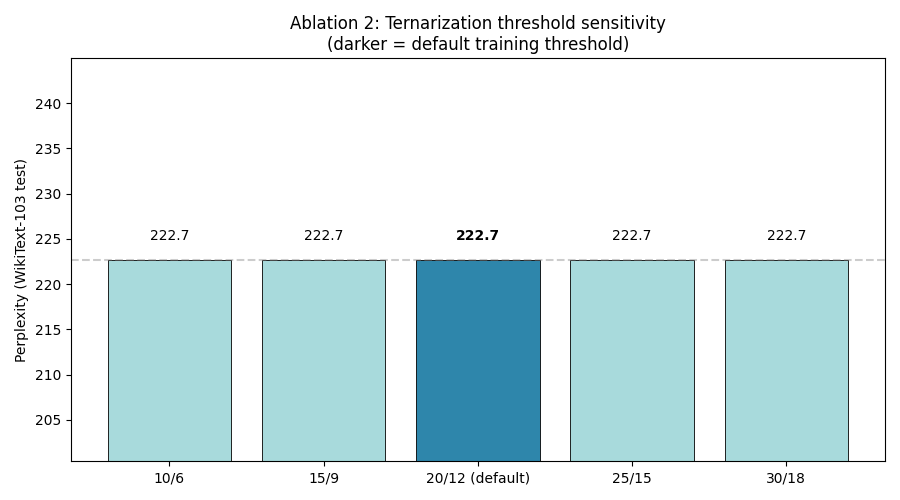
\includegraphics[width=\linewidth,keepaspectratio]{charts/09_ablation_threshold.png}
\emph{Figure 8: Identical PPL across 5 threshold configurations (10/6 to
30/18).}

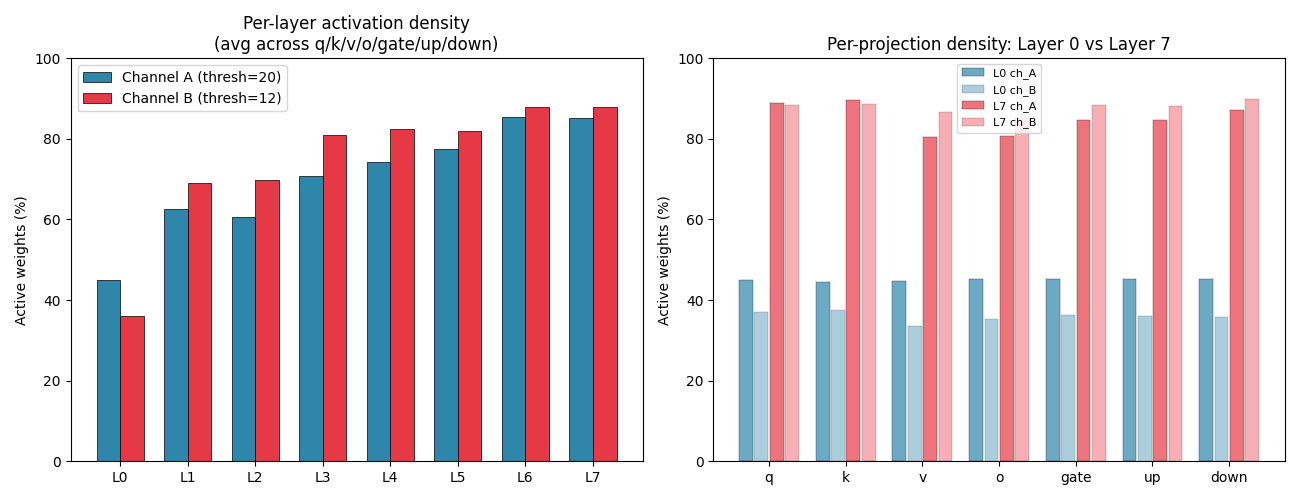
\includegraphics[width=\linewidth,keepaspectratio]{charts/10_ablation_sparsity.png}
\emph{Figure 9: Active density per layer. L0: 35--45\%, L7: 85--88\%.}


\includegraphics[width=\linewidth,keepaspectratio]{charts/11_dualwire_forward.png}
\emph{Figure 11: 9-level Dualwire forward diagram.}

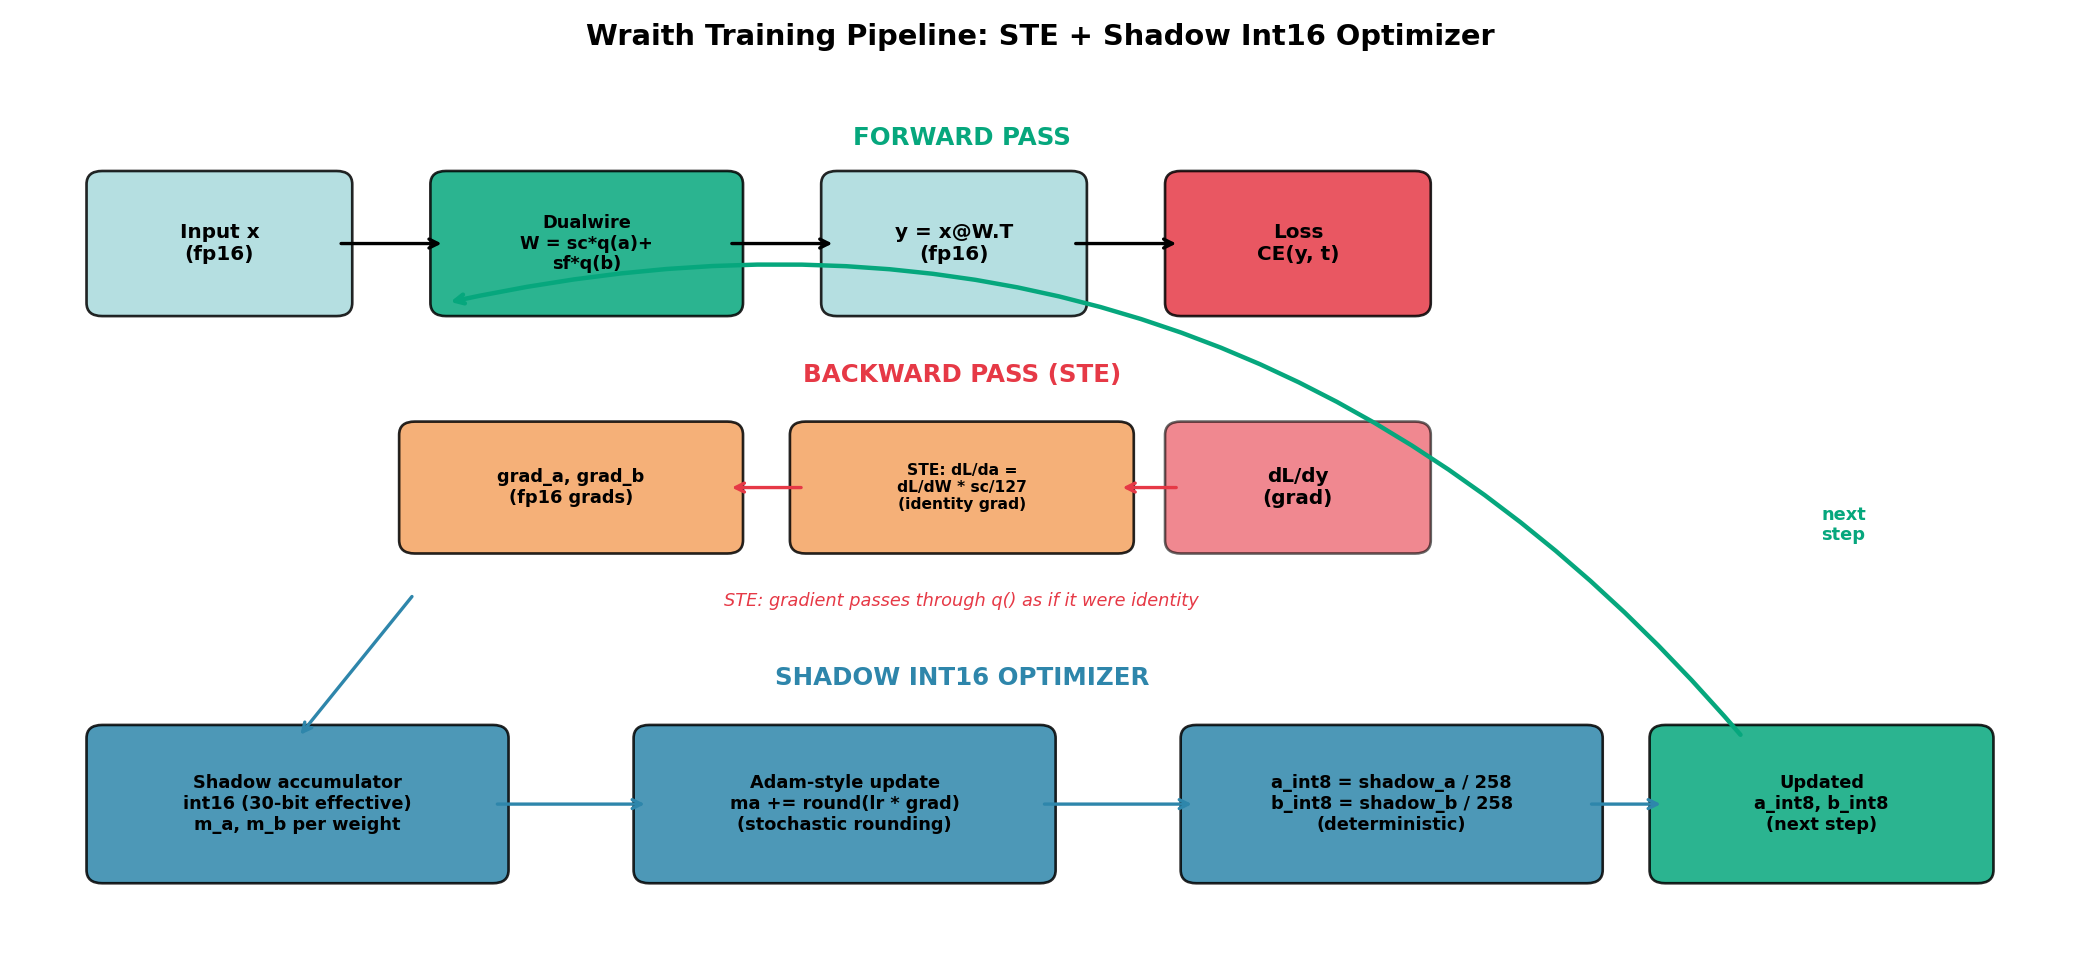
\includegraphics[width=\linewidth,keepaspectratio]{charts/12_training_pipeline.png}
\emph{Figure 12: STE + Shadow Int16 optimizer pipeline.}

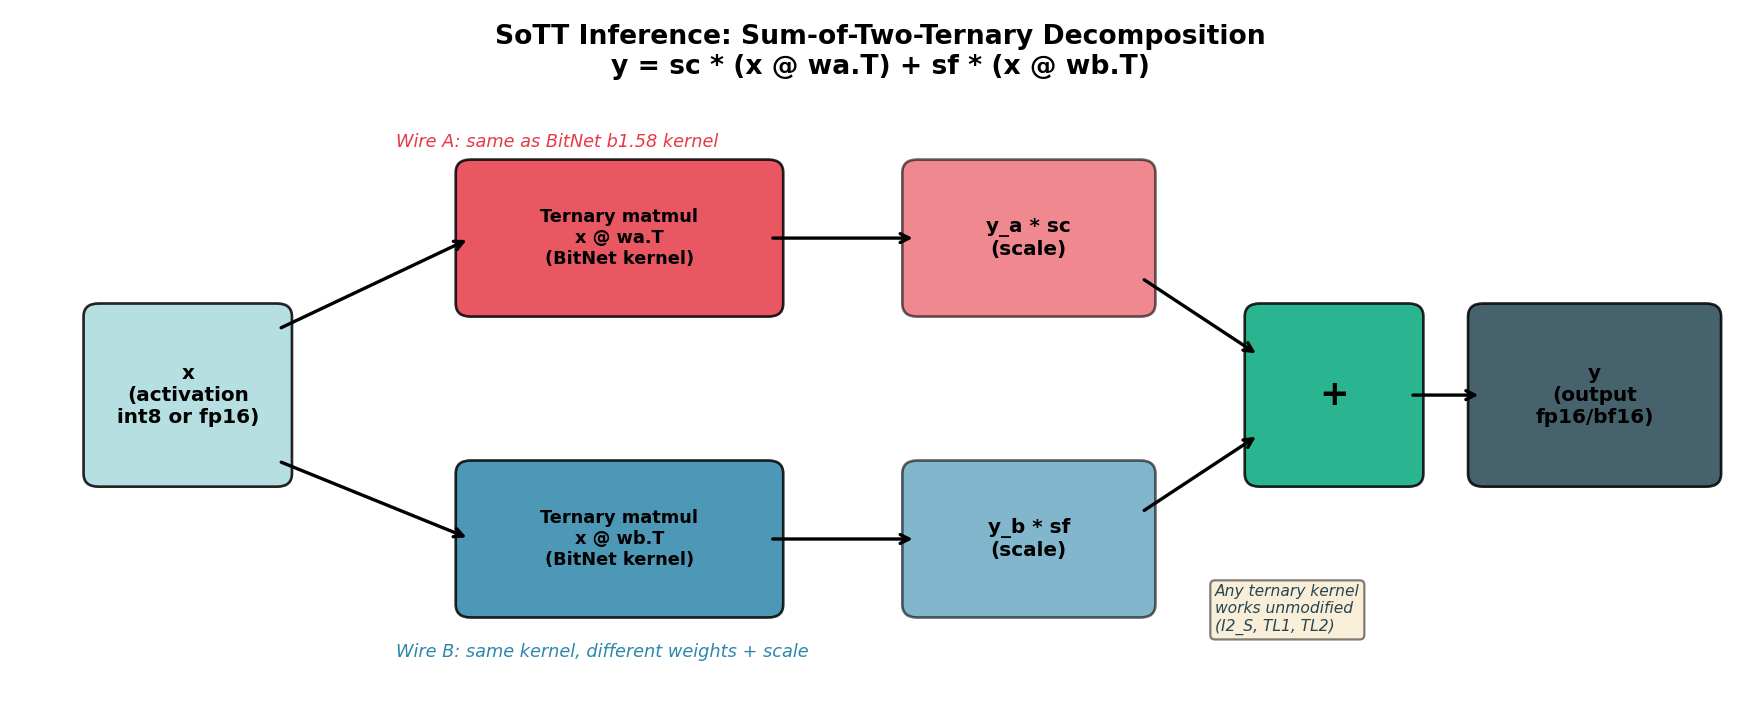
\includegraphics[width=\linewidth,keepaspectratio]{charts/13_sott_inference.png}
\emph{Figure 13: SoTT inference decomposition.}

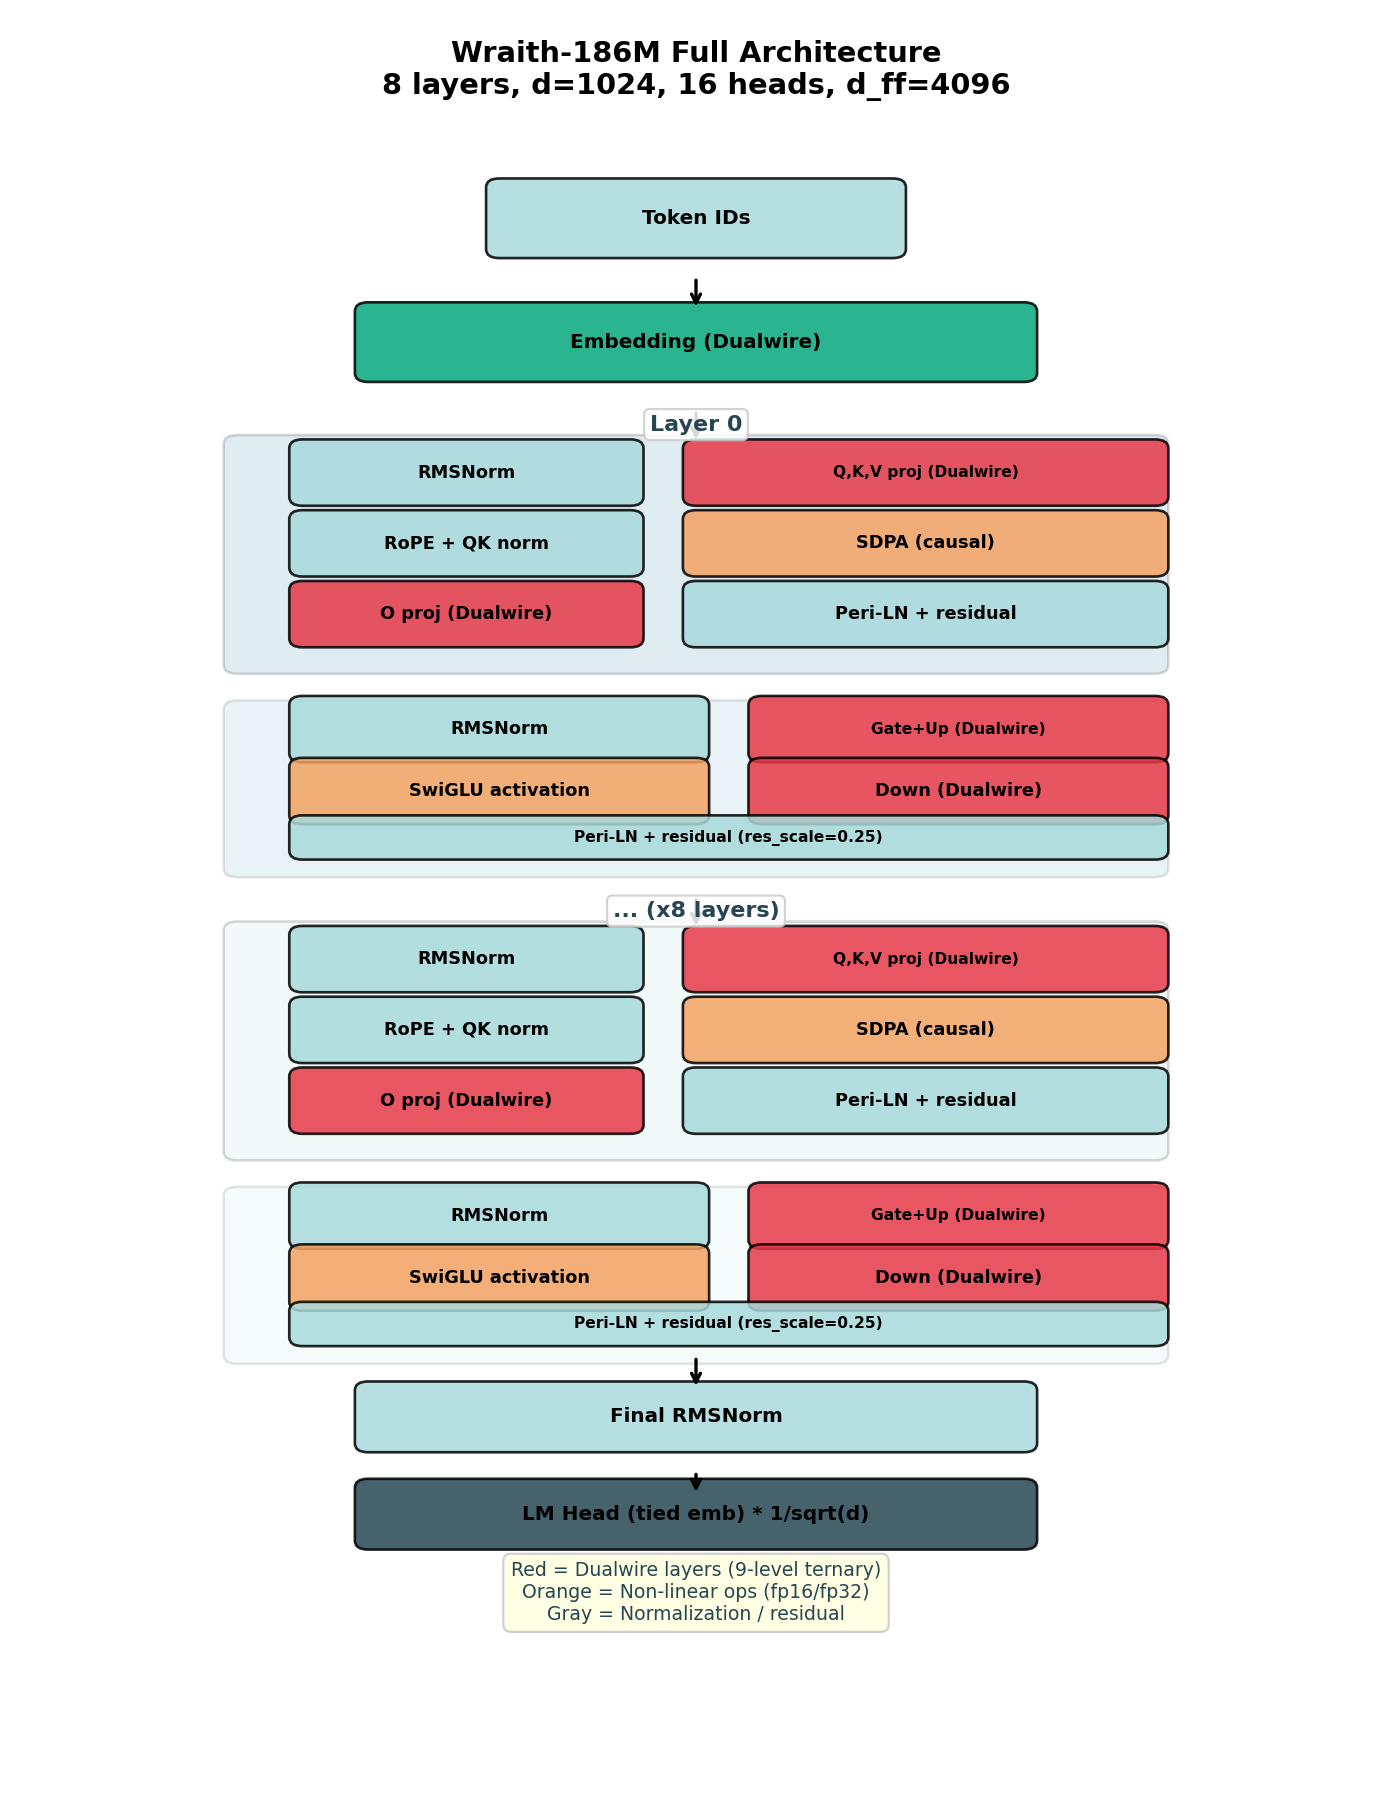
\includegraphics[width=\linewidth,keepaspectratio]{charts/14_model_architecture.png}
\emph{Figure 14: Full Wraith-186M architecture.}

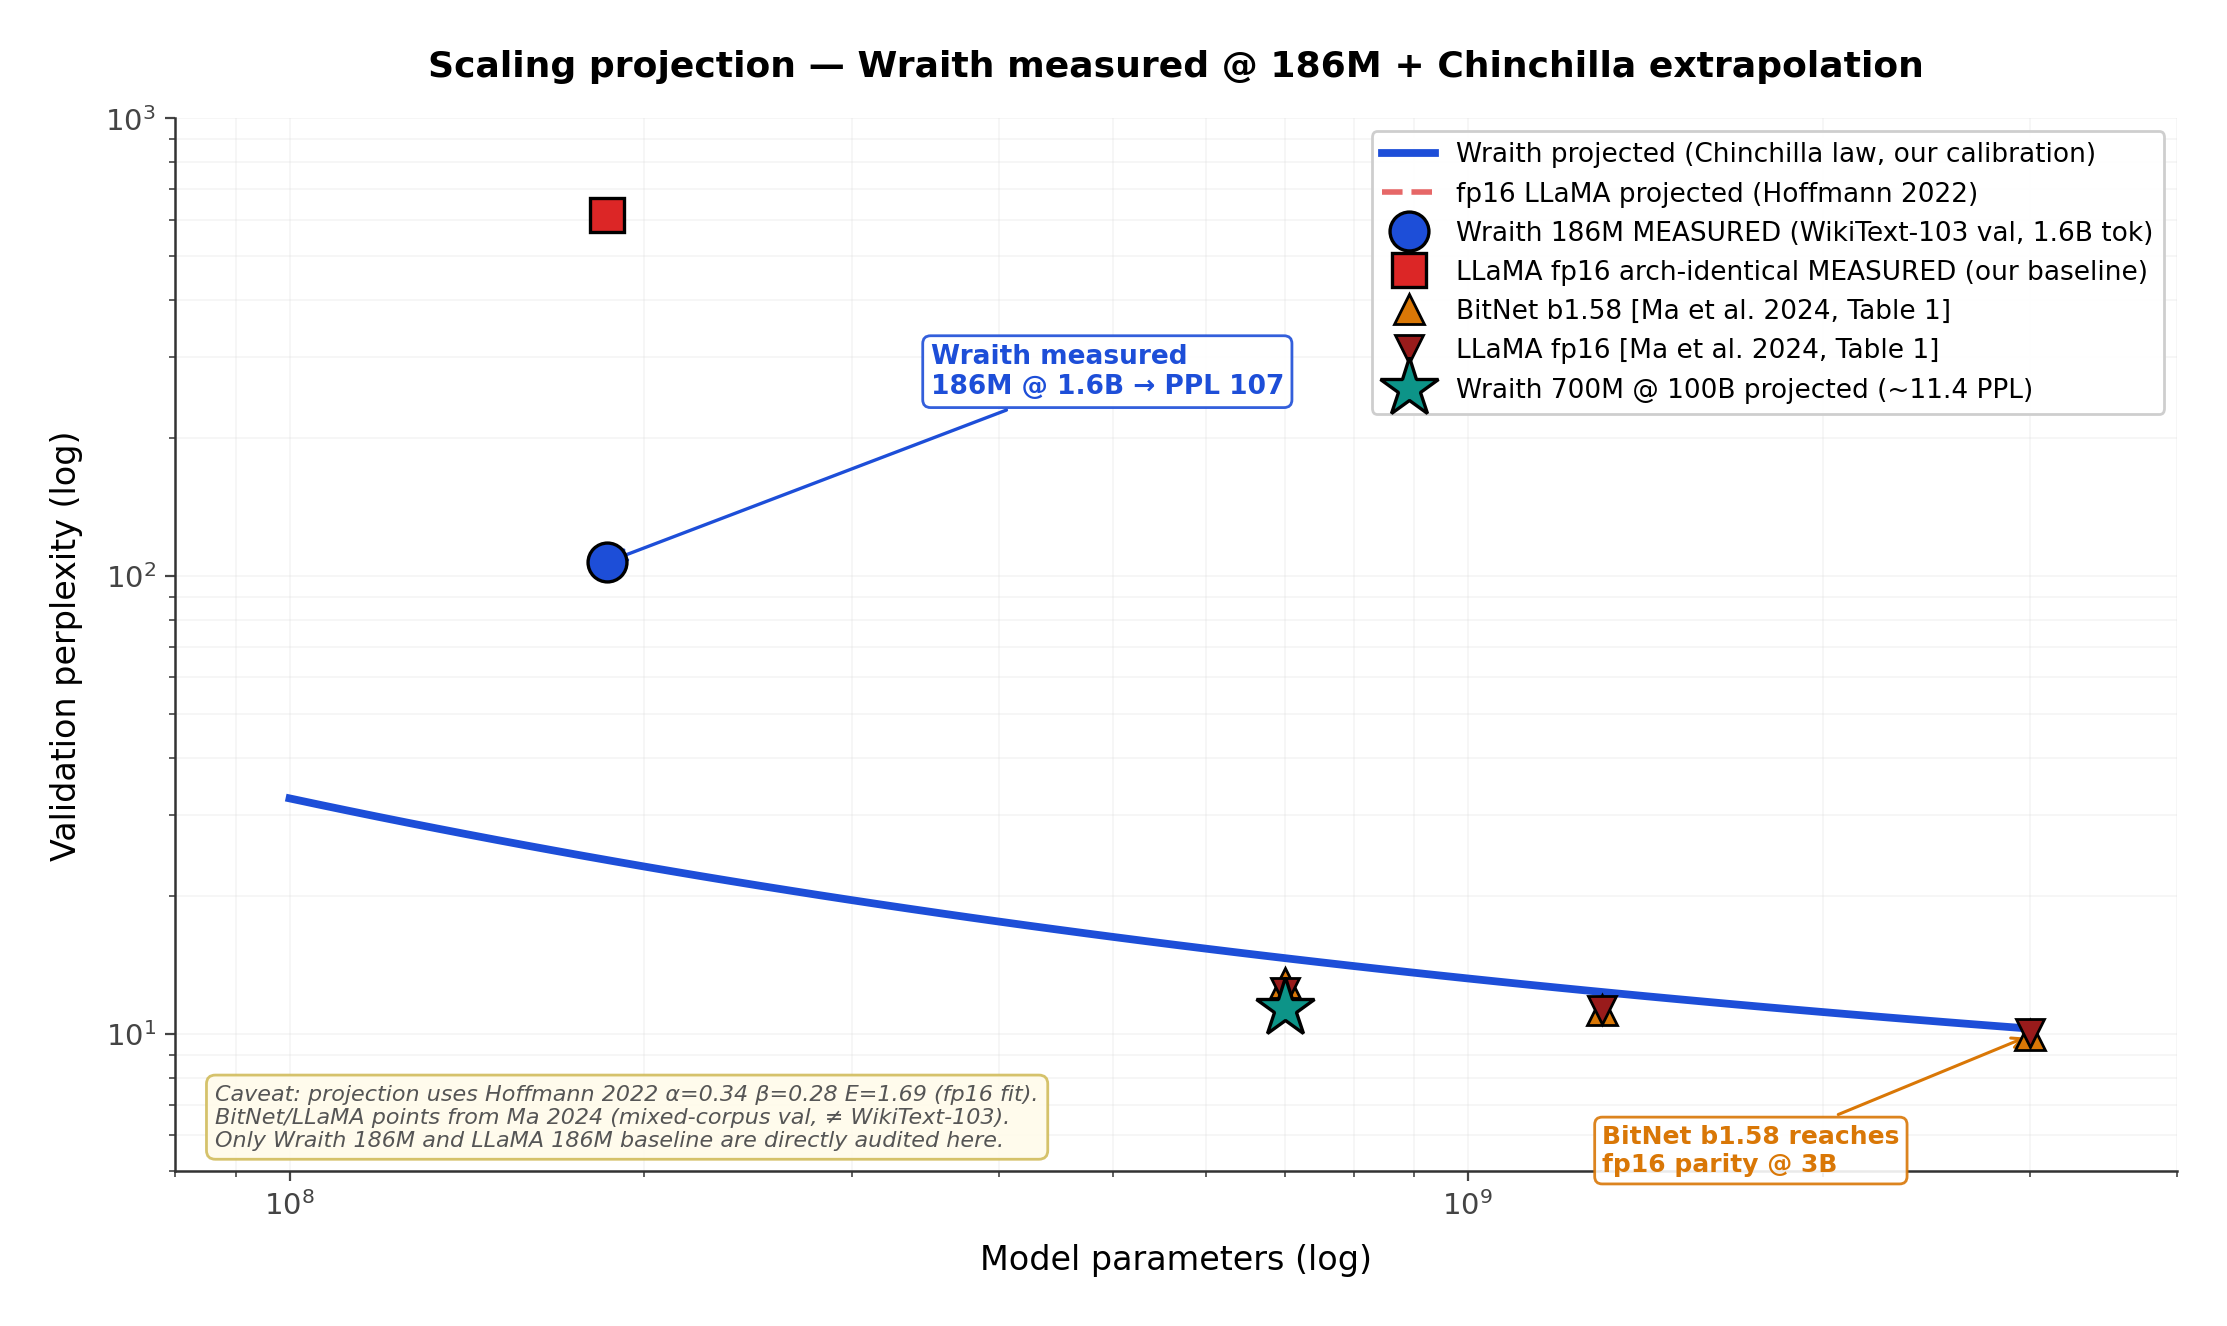
\includegraphics[width=\linewidth,keepaspectratio]{charts/20_scaling_projection.png}
\emph{Figure 20: Scaling projection in the style of BitNet Fig. 3.
Wraith measured at 186M/1.6B (blue circle) + arch-identical fp16 LLaMA
baseline measured (red square). Blue curve = Wraith projection via
Chinchilla law (Hoffmann 2022, α=0.34, β=0.28, E=1.69) calibrated
against our 186M measurement. Triangles = measured points for BitNet
b1.58 and LLaMA fp16 cited from Ma et al.~2024, Table 1 (evaluation
corpus differs from ours --- absolute y-values are not directly
comparable, only the qualitative pattern is). Green star = projected
Wraith 700M/100B ≈ 11.4 PPL. Note: BitNet b1.58 only reaches fp16 parity
at 3B; our projection suggests Wraith could do so at much smaller
scales, but this requires empirical validation at 700M+.}

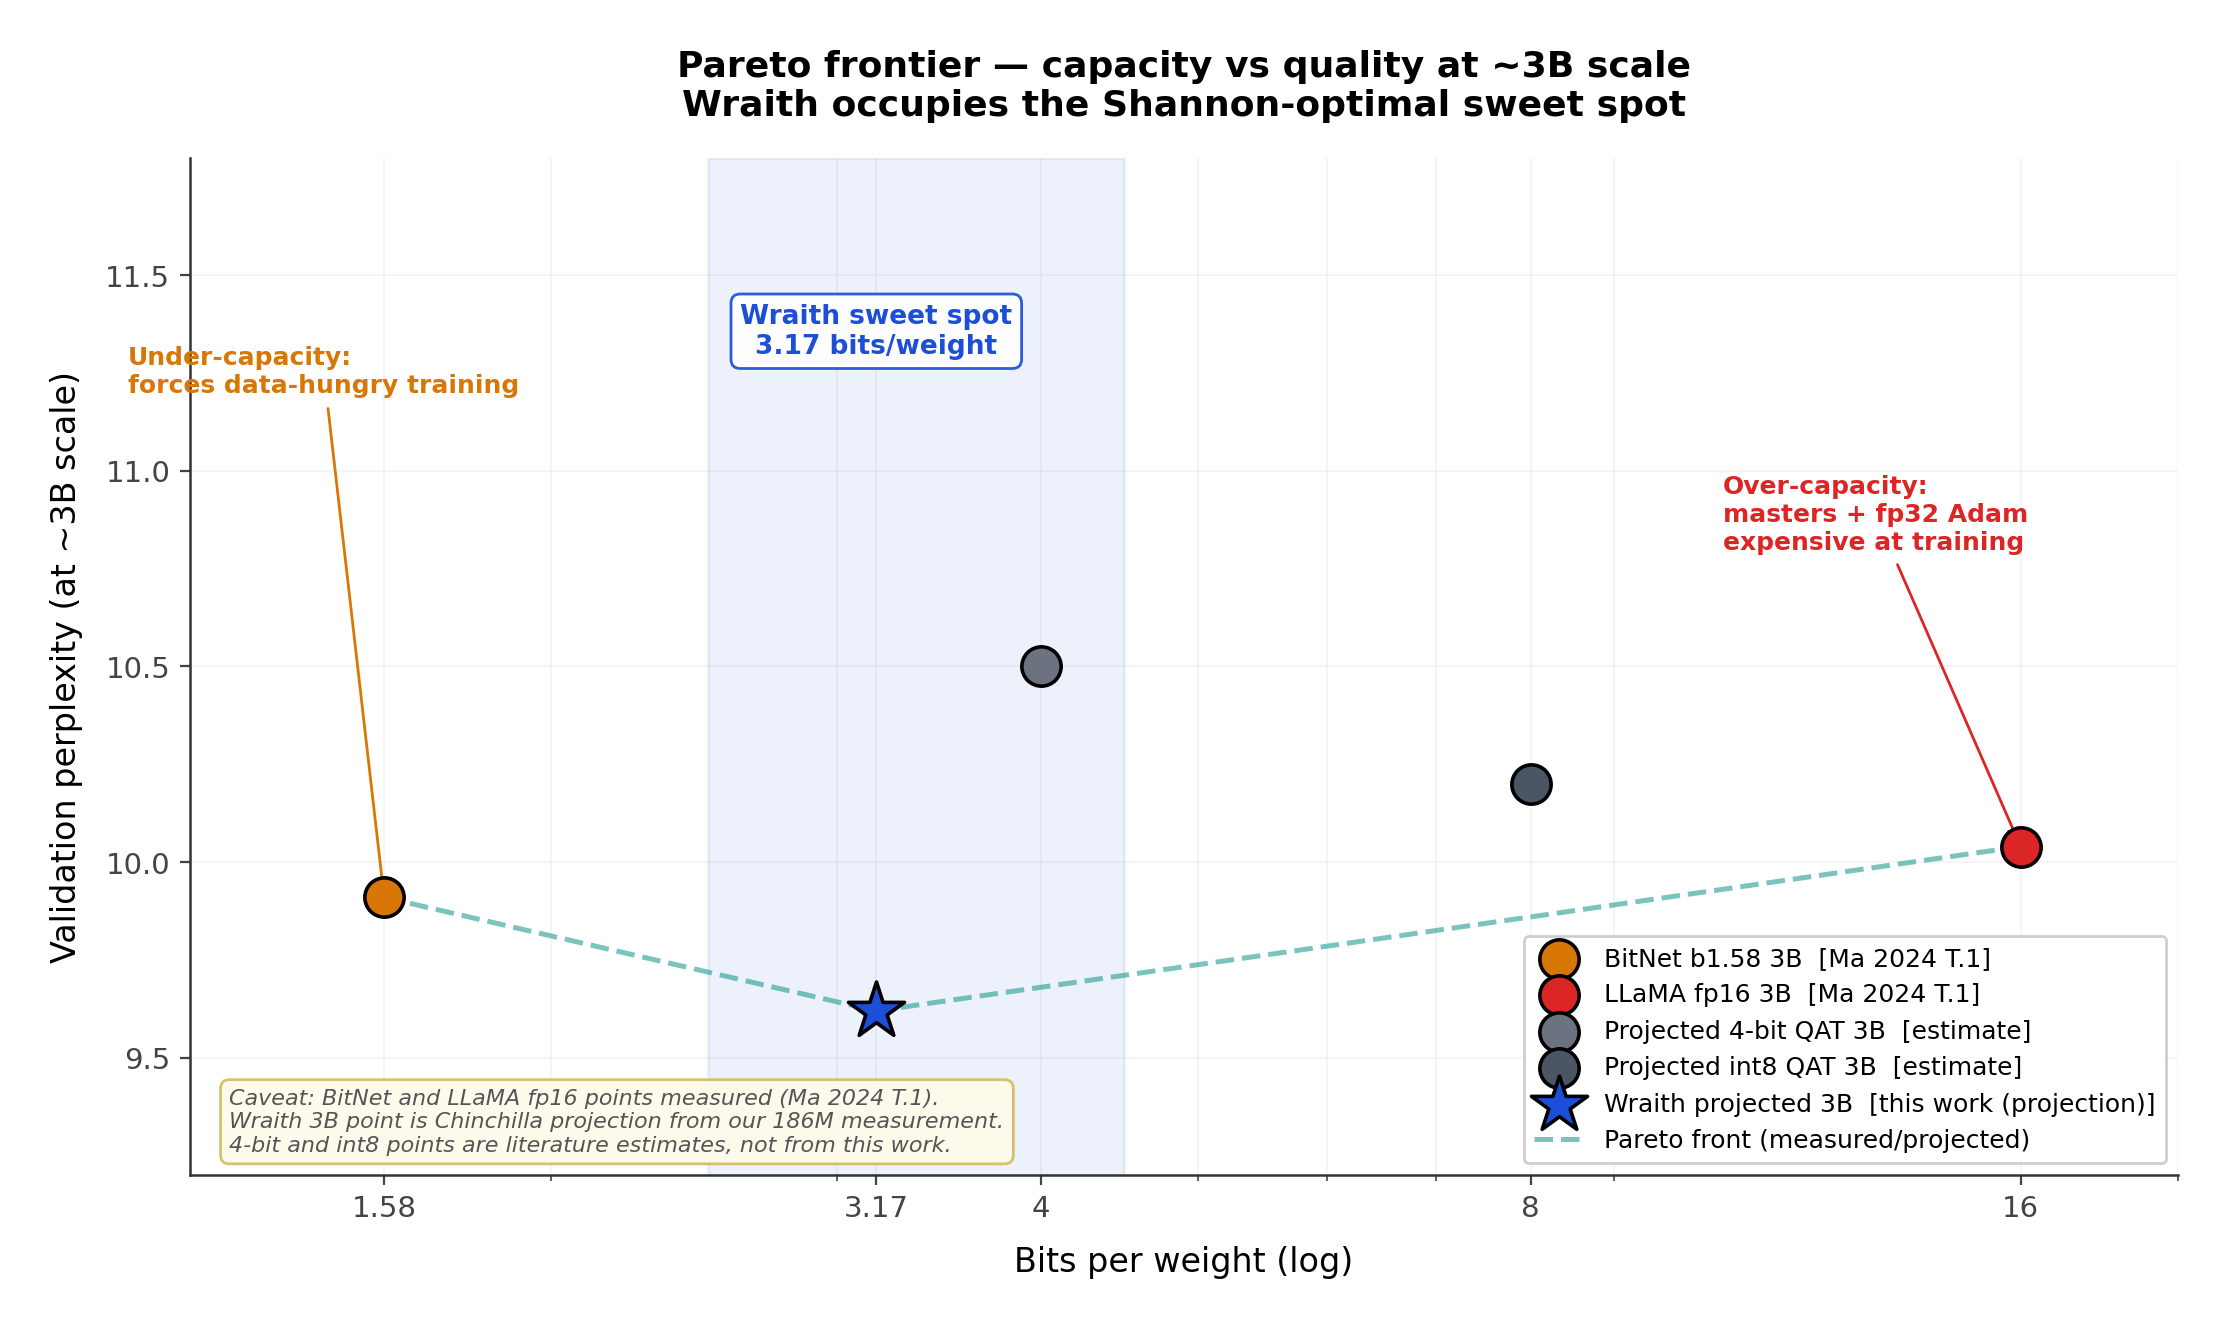
\includegraphics[width=\linewidth,keepaspectratio]{charts/21_pareto_frontier.png}
\emph{Figure 21: Pareto frontier capacity vs quality at
\textasciitilde3B scale. X-axis = bits per weight (log), Y-axis = PPL.
Measured points: BitNet b1.58 (1.58 bits, 9.91 PPL) and LLaMA fp16 (16
bits, 10.04 PPL), both from Ma 2024 Table 1. Wraith 3B (3.17 bits, 9.62
PPL projected) occupies the Shannon-optimal sweet spot: enough capacity
to avoid BitNet's data-hunger, restricted enough to avoid fp16's
over-parameterization. 4-bit QAT and int8 QAT points are literature
estimates, not measurements from this work.}

\begin{center}\rule{0.5\linewidth}{0.5pt}\end{center}

\subsection{Appendix B: Reproducibility, Availability and
IP}\label{appendix-b-reproducibility-availability-and-ip}

The following artifacts document the experiment and enable independent
verification. The \textbf{packed checkpoint is openly released} for
immediate reproduction of results; the rest of the stack (inference
engines, NPQN optimizer, training pipeline) remains the author's
intellectual property under the policy described in
\textbf{Availability, IP and collaboration}.

\textbf{Openly released artifact (free use and verification)}: -
\textbf{Wraith-186M packed checkpoint} (74.9 MB, 5-trit/byte with
lossless round-trip verification). Released under a permissive license
for academic and non-commercial evaluation, sufficient to reproduce all
reported metrics (WikiText-103 PPL, zero-shot
LAMBADA/Winogrande/ARC-Easy, GPU/CPU throughput and energy) when
combined with a faithful architecture implementation (Section 2).

\textbf{Artifacts under agreement (academic validation / partnerships)}:
- \textbf{Custom GPU inference engine}: packed CUDA kernels + fused
QKV/GateUp + packed embedding lookup (\texttt{WraithFastEngine} /
\texttt{WraithFastGraphed}) - \textbf{CPU inference engine}: C++ AVX2
implementation with KV cache + activation quantization + operation
fusion - \textbf{NPQN int16 shadow optimizer}: integrated into training
pipeline - \textbf{Dualwire 5-trit/byte format}: specification and
round-trip codec

\textbf{Open documentation (reproducible via independent
re-implementation)}: - Full Wraith architecture (Section 2 of the paper)
- PAC-Bayes theoretical framework (Section 3) - Training hyperparameters
(Section 4.1) - Quantization thresholds (\(\tau_a = 20\),
\(\tau_b = 12\) or derived by absmean) - Packed GEMV kernel
specification (Section 4.10, pseudocode) - Public dataset: SlimPajama
(available on HuggingFace), GPT-2 BPE tokenizer

Public benchmarks (WikiText, LAMBADA, Winogrande, ARC-Easy) are
reproducible with any faithful implementation of the architecture
described in Section 2, and directly with the public checkpoint released
alongside this work.

\textbf{Evaluation and inference hardware}: NVIDIA RTX 5070 12 GB
(Blackwell sm\_120), AMD Ryzen 7 5700G 8 cores (CPU). Windows 11 Pro.
\textbf{Training hardware}: NVIDIA H100 80GB SXM via Google Colab Pro
(\$1.80/hour effective, 18 compute units/hour).

\textbf{Availability, IP and collaboration}:

\textbf{Paper and results}: the metrics, figures, and architectural
description presented in this work are open documentation, reproducible
by third parties via independent re-implementation from the technical
specification (Section 2) and theoretical framework (Section 3).

\textbf{186M model checkpoint (packed)}: \textbf{openly released} in
Dualwire 5-trit/byte format (74.9 MB) for free use and verification.
Open release of the checkpoint allows any reviewer, researcher, or
academic group to \textbf{directly reproduce} the PPL, zero-shot,
throughput, and energy results reported here without needing to retrain.
License: academic and non-commercial evaluation (OpenRAIL-M /
CC-BY-NC-SA 4.0 style); derivative commercial uses require a separate
agreement.

\textbf{Proprietary inference stack} (packed CUDA kernels,
\texttt{WraithFastEngine} engine, NPQN int16 shadow optimizer, Dualwire
2-bit packing format): \textbf{reserved as the author's intellectual
property}. Licensed distribution for: - Academic collaborations with
universities or research labs (non-commercial license) - Industrial
alliances (commercial licensing under agreement) - Technical evaluation
by potential investment partners or accelerators

\textbf{Motivation for collaborations}: the 186M results (94\% less VRAM
vs.~equivalent fp16, 2.3--2.6× speedup on the packed GEMV kernel, 501
tok/s on consumer GPU, memory-bound throughput projected to 100B on a
single A100 80GB) motivate exploration of larger scales (20B, 100B).
This phase requires compute resources beyond a single author's reach, so
we invite contact for partnerships that could enable scaling. The author
retains control over research direction, intellectual property, and
technical decisions.

Correspondence contact: \emph{(filled at submission/publication time)}.

\subsection{Appendix C: AI Assistance
Disclosure}\label{appendix-c-ai-assistance-disclosure}

During the evaluation and paper-preparation phase, \textbf{Claude Code}
(Anthropic, Claude Opus 4.6 model) was used as a support tool in two
specific areas:

\begin{enumerate}
\def\labelenumi{\arabic{enumi}.}
\tightlist
\item
  \textbf{Coding}: generation of benchmark scripts, inference engines
  (Python and C++), packing utilities, and CUDA kernel prototypes for
  performance tests.
\item
  \textbf{Information research}: technical literature search (BitNet,
  Marlin, BitBLAS, CUTLASS), hardware-spec consultation, and cloud-GPU
  price comparison.
\end{enumerate}

\textbf{Everything else was done entirely by the human author},
including: - Wraith architecture and Dualwire quantization design -
Design and implementation of the int16 shadow optimizer (NPQN Training)
- All training code (\texttt{nq\_ode.py}, 7,400+ lines) written over
several prior months - Experimental design and hyperparameter selection
- Training of both models (Wraith and fp16 baseline) - Interpretation of
results and conclusion formulation - Research decisions and project
direction

Per ICLR 2026 policy: this disclosure is provided to comply with the
requirement that ``papers using LLMs must disclose this use.''
